\documentclass[letterpaper,12pt,oneside,final]{book}
\usepackage{ragged2e}
%%
%%  Template de mémoire de maîtrise ou thèse de doctorat.
%%  Normalement, il n'est pas nécessaire de modifier ce document
%%  sauf pour changer les noms des fichiers à inclure.
%%
%%  Version: 2014-10-28
%%
%%  Accepte les caractères accentués dans le document (UTF-8).
\usepackage[utf8]{inputenc}
%%
%% Support pour l'anglais et le français (français par défaut).
%\usepackage[cyr]{aeguill}
\usepackage{lmodern}      % Police de caractères plus complète et généralement indistinguable visuellement de la police standard de LaTeX (Computer Modern).
\usepackage[T1]{fontenc}  % Bon encodage des caractères pour qu'Acrobat Reader reconnaisse les accents et les ligatures telles que ffi.
\usepackage[english,frenchb]{babel} % le langage par défaut est le dernier de la liste, c'est-à-dire français
%%
%% Charge le module d'affichage graphique.
\usepackage{graphicx}
\usepackage{epstopdf}  % Permet d'utiliser des .eps avec pdfLaTeX.
%%
%% Recherche des images dans les répertoires.
\graphicspath{{./images/}{./dia/}{./gnuplot/}}
%%
%% Un float peut apparaître seulement après sa définition, jamais avant.
\usepackage{flafter,placeins}
%%
%% Utilisation de natbib pour les citations et la bibliographie.
\usepackage{natbib}
%%
%% Autres packages.
\usepackage{amsmath,color,soulutf8,longtable,colortbl,setspace,ifthen,xspace,url,pdflscape}
%%
%% Support des acronymes.
\usepackage[nolist]{acronym}
\onehalfspacing                % Interligne 1.5.
%%
\usepackage{listings}

%% Définition d'un style de page avec seulement le numéro de page à
%% droite. On s'assure aussi que le style de page par défaut soit
%% d'afficher le numéro de page en haut à droite.
\usepackage{fancyhdr}
\fancypagestyle{pagenumber}{\fancyhf{}\fancyhead[R]{\thepage}}
\renewcommand\headrulewidth{0pt}
\makeatletter
\let\ps@plain=\ps@pagenumber
\makeatother
%%
%% Module qui permet la création des bookmarks dans un fichier PDF.
%\usepackage[dvipdfm]{hyperref}
\usepackage{hyperref}
\usepackage{caption}  % Hyperlien vers la figure plutôt que son titre.
\makeatletter
\providecommand*{\toclevel@compteur}{0}
\makeatother
%%
%% Définitions spécifiques au format de rédaction de Poly.
\usepackage{MemoireThese}
%%
%% Définitions spécifiques à l'étudiant.
%% -----------------------------------
%% ---> A MODIFIER PAR L'ETUDIANT <---
%% -----------------------------------
%%
%% Commandes qui affichent le titre du document, le nom de l'auteur, etc.
\newcommand\monTitre{TRACING COMPARISON USING DATA MINING TECHNIQUES}
\newcommand\monPrenom{Isnaldo Francisco}
\newcommand\monNom{de Melo Junior}
\newcommand\monDepartement{génie informatique et génie logiciel}
\newcommand\maDiscipline{génie informatique}
\newcommand\monDiplome{M}        % (M)aîtrise ou (D)octorat
\newcommand\anneeDepot{2017}
\newcommand\moisDepot{june}
\newcommand\monSexe{M}           % "M" ou "F"
\newcommand\PageGarde{N}         % "O" ou "N"
\newcommand\AnnexesPresentes{N}  % "O" ou "N". Indique si le document comprend des annexes.
\newcommand\mesMotsClef{Liste,de,mot-clés,séparés,par,des,virgules}
%%
%%  DEFINITION DU JURY
%%
%%  Pour la définition du jury, les macros suivantes sont definies:
%%  \PresidentJury, \DirecteurRecherche, \CoDirecteurRecherche, \MembreJury, \MembreExterneJury
%%
%%  Toutes les macros prennent 4 paramètres: Sexe (M/F), Prénom, Nom, Titres
\newcommand\monJury{\PresidentJury{M}{Prénom}{NOM}{Doct.}\\
\DirecteurRecherche{F}{Michel}{Dagenais}{Ph.~D.}\\
\MembreJury{M}{Prénom}{Nom}{Ph.~D.}}

\ifthenelse{\equal{\monDiplome}{M}}{
\newcommand\monSujet{Mémoire de maîtrise}
\newcommand\monDipl{Maîtrise ès sciences appliquées}
}{
\newcommand\monSujet{Thèse de doctorat}
\newcommand\monDipl{Philosophi\ae{} Doctor}
}
%%
%% Informations qui sont stockées dans un fichier PDF.
\hypersetup{
  pdftitle={\monTitre},
  pdfsubject={\monSujet},
  pdfauthor={\monPrenom{} \monNom},
  pdfkeywords={\mesMotsClef},
  bookmarksnumbered,
  pdfstartview={FitV},
  hidelinks,
  linktoc=all
}
%%
%% Il y a un document par chapitre du mémoire.
%%
\begin{document}
%%
%% Page de titre du mémoire.
\frontmatter
% Compte optionellement la page de garde dans la pagination.
\ifthenelse{\equal{\PageGarde}{O}}{\addtocounter{page}{1}}{}
\thispagestyle{empty}%
\begin{center}%
\vspace*{\stretch{1}}
UNIVERSITÉ DE MONTRÉAL\\
\vspace*{\stretch{1}}
\MakeUppercase{\monTitre}\\
\vspace*{\stretch{1}}
\MakeUppercase{\monPrenom~\monNom}\\
DÉPARTEMENT DE \MakeUppercase{\monDepartement}\\
ÉCOLE POLYTECHNIQUE DE MONTRÉAL\\
\vspace*{\stretch{1}}
\ifthenelse{\equal{\monDiplome}{M}}{MÉMOIRE PRÉSENTÉ}{THÈSE PRÉSENTÉE} EN VUE DE L'OBTENTION\\
DU DIPLÔME DE \MakeUppercase{\monDipl}\\
(\MakeUppercase{\maDiscipline})\\
\MakeUppercase{\moisDepot} \anneeDepot
\end{center}%
\vspace*{\stretch{1}}
\copyright~\monPrenom~\monNom, \anneeDepot.
%%
%% Identification des membres du jury.
%%
\newpage\thispagestyle{empty}%
\begin{center}%
\vspace*{\stretch{2}}
\ul{UNIVERSITÉ DE MONTRÉAL}\\
\vspace*{\stretch{1}}
\ul{ÉCOLE POLYTECHNIQUE DE MONTRÉAL}\\
\vspace*{\stretch{2}}
Ce\ifthenelse{\equal{\monDiplome}{M}}{~mémoire intitulé}{tte thèse intitulée}:\\
\vspace*{\stretch{1}}
\MakeUppercase{\monTitre}\\
\vspace*{\stretch{2}}
\end{center}%
\begin{flushleft}
présenté\ifthenelse{\equal{\monDiplome}{M}}{}{e}
par:~\ul{\mbox{\MakeUppercase{\monNom} \monPrenom}}\\
en vue de l'obtention du diplôme de:~\ul{\mbox{\monDipl}}\\
a été dûment accepté\ifthenelse{\equal{\monDiplome}{M}}{}{e} par le jury d'examen constitué de:\end{flushleft}
\vspace*{\stretch{2}}
\monJury
%%
\pagestyle{pagenumber}%
\begin{otherlanguage}{english}

\begin{flushright}

Maria, Maria\\
É o som, é a cor, é o suor\\
É a dose mais forte e lenta\\
De uma gente que ri\\
Quando deve chorar\\
E não vive, apenas aguenta\\

 
Amar é mudar a alma de lugar
Quintana, Mario
\end{flushright}
\end{otherlanguage}
   
%% Dédicace
%%
%% La dédicace est un hommage que l'auteur souhaite
%% rendre à une ou plusieurs personnes de son choix.
%%
\chapter*{DEDICATION}\thispagestyle{headings}
\addcontentsline{toc}{compteur}{DEDICATION}
\begin{flushright}
  \itshape
  \begin{figure}[h]
          \flushright
            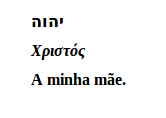
\includegraphics[width=0.27\textwidth]{figures/dedication.png}
            \label{fig:dedication}
    \end{figure}
\end{flushright}
          % Dédicace du document.
% Remerciements
%
%   Grâce aux remerciements, l'auteur attire l'attention du lecteur
% sur l'aide que certaines personnes lui ont apportée, sur leurs
% conseils ou sur toute autre forme de contribution lors de la
% réalisation de son mémoire. Le cas échéant, c'est dans cette section
% que le candidat doit témoigner sa reconnaissance à son directeur de
% recherche, aux organismes dispensateurs de subventions ou aux
% entreprises qui lui ont accordé des bourses ou des fonds de
% recherche.
\chapter*{ACKNOWLEDGEMENTS}\thispagestyle{headings}
\addcontentsline{toc}{compteur}{ACKNOWLEDGEMENTS}
%
I would like to thank all those who have supported me during my graduate studies. Specially to Professor Michel Dagenais, who gave me his support and advice for this research.
 
I acknowledge all my committee members: Professor Michel Gagnon and Professor Daniel Aloise to evaluate my research contribution.
 
 Also I would like to thank my colleagues at DORSAL laboratory, for their valuable comments on my development. They’ve helped making my path possible with their precious comments and considerations.
 
Special thanks for Gabriel A., my uncle Nacib Asseff, and Leticia R. for their tremendous support during my studies and help in the several challenges faced.
 
I also would like to praise the Ecole Polytechnique de Montreal and the department of Computer and Software Engineering for giving me the opportunity of studying and working here. 
 
 Last but not the least; I would like to acknowledge my mother, Maria Pereira de Assis, for her imperative support throughout my path. 
 
\begin{flushleft}
\textit{Venimus, Vidimus, Deus vicit}
\end{flushleft}
 % Remerciements.
% Résumé du mémoire.
%
%   Le résumé est un bref exposé du sujet traité, des objectifs visés,
% des hypothèses émises, des méthodes expérimentales utilisées et de
% l'analyse des résultats obtenus. On y présente également les
% principales conclusions de la recherche ainsi que ses applications
% éventuelles. En général, un résumé ne dépasse pas quatre pages.
%
%   Le résumé doit donner une idée exacte du contenu du mémoire ou de la thèse. Ce ne
% peut pas être une simple énumération des parties du document, car il
% doit faire ressortir l'originalité de la recherche, son aspect
% créatif et sa contribution au développement de la technologie ou à
% l'avancement des connaissances en génie et en sciences appliquées.
% Un résumé ne doit jamais comporter de références ou de figures.
\chapter*{RÉSUMÉ}\thispagestyle{headings}
\addcontentsline{toc}{compteur}{RÉSUMÉ}

La performance est devenue une question cruciale sur le développement, le test et la maintenance des logiciels. Pour répondre à cette préoccupation, les développeurs et les testeurs utilisent plusieurs outils pour améliorer les performances ou suivre les bogues liés à la performance.\\
L'utilisation de méthodologies comparatives telles que Flame Graphs fournit un moyen formel de vérifier les causes des régressions et des problèmes de performance. L'outil de comparaison fournit des informations pour l'analyse qui peuvent être utilisées pour les améliorer par un mécanisme de profilage profond, comparant habituellement une donnée normale avec un profil de profil anormal.\\
D'autre part, le mécanisme de traçage est un mécanisme de tendance visant à enregistrer des événements dans le système et à réduire les frais généraux de son utilisation. Le registre de cette information peut être utilisé pour fournir aux développeurs des données pour l'analyse de performance. Cependant, la quantité de données fournies et les connaissances requises à comprendre peuvent constituer un défi pour les méthodes et les outils d'analyse actuels.
La combinaison des deux méthodologies, un mécanisme comparatif de profilage et un système de traçabilité peu élevé peut permettre d'évaluer les causes des problèmes répondant également à des exigences de performance strictes en même temps. La prochaine étape consiste à utiliser ces données pour développer des méthodes d'analyse des causes profondes et d'identification des goulets d'étranglement.\\
L'objectif de ce projet de recherche est d'automatiser le processus d'analyse des traces et d'identifier automatiquement les différences entre les groupes d'exécutions. La solution présentée souligne les différences dans les groupes présentant une cause possible de cette différence, l'utilisateur peut alors bénéficier de cette revendication pour améliorer les exécutions.\\
Nous présentons une série de techniques automatisées qui peuvent être utilisées pour trouver les causes profondes des variations de performance et nécessitant des interférences mineures ou non humaines. L'approche principale est capable d'indiquer la performance en utilisant une méthodologie de regroupement comparative sur les exécutions et a été appliquée sur des cas d'utilisation réelle. La solution proposée a été mise en œuvre sur un cadre d'analyse pour aider les développeurs à résoudre des problèmes similaires avec un outil différentiel de flamme.\\
À notre connaissance, il s'agit de la première tentative de corréler les mécanismes de regroupement automatique avec l'analyse des causes racines à l'aide des données de suivi.\\
Dans ce projet, la plupart des données utilisées pour les évaluations et les expériences ont été effectuées dans le système d'exploitation Linux et ont été menées à l'aide de Linux Trace Toolkit Next Generation (LTTng) qui est un outil très flexible avec de faibles coûts généraux.      % Résumé du sujet en français.
% Abstract
%
%   Résumé de la recherche écrit en anglais sans être
% une traduction mot à mot du résumé écrit en français.

\chapter*{ABSTRACT}\thispagestyle{headings}
\addcontentsline{toc}{compteur}{ABSTRACT}
%
\begin{otherlanguage}{english}

Performance has become a crucial matter on software development, testing and maintenance. To address this concern, developers and testers use several tools to improve the performance or track performance related bugs. \\
The use of comparative methodologies such as Flame Graphs provides a formal way to verify causes of regressions and performance issues. The comparison tool provides information for analysis that can be used to improve them by a deep profiling mechanism, usually comparing a normal with an abnormal profiling data.
On the other hand, Tracing mechanism is a trend mechanism targeting to record events in the system and reduce the overhead of its utilization. The record of this information can be used to supply developers with data for performance analysis. However, the amount of data provided and the requirement knowledge to understand may present a challenge for the current analysis methods and tools.\\
Combining both methodologies, a comparative mechanism of profiling and a low overhead trace system can enable evaluate causes of issues also meeting stringent performance requirements at the same time. The next step is to use this data to develop methods to root cause analysis and bottleneck identification.
The objective of this research project is to automate the process of trace analysis and automatic identification of differences among a groups of executions. The presented solution highlight differences in the groups presenting a possible cause of this difference, the user can then benefit from this claim to improve the executions. \\
We present a series of automated techniques that can be used to find the root causes of performance variations and that requiring small or non human interference. The main approach is capable to indicate the performance cause using a comparative grouping methodology on the executions and was applied on real use cases. The proposed solution was implemented on an analysis framework to help developers on similar problems together with a differential flame graph tool. 
To our knowledge, this is the first attempt to correlate automatic grouping mechanisms with root cause analysis using tracing data. In this project, most of the data used for evaluations and experiments were done in Linux Operating System and were conducted using the Linux Trace Toolkit Next Generation (LTTng) which is a very flexible tool with low overhead.


\end{otherlanguage}
          % Résumé du sujet en anglais.

\chapter*{CO-AUTHORSHIP}\thispagestyle{headings}
\addcontentsline{toc}{compteur}{CO-AUTHORSHIP}
%
\begin{otherlanguage}{english}

The following work was done in collaboration:\\
Title: Automated Performance Deviation Detection Across Software Versions Releases\\
Authors: Abderrahmane Benbachir, Isnaldo Francisco de Melo, Michel Dagenais and Bram Adams. This paper was accepted in the conference Software Quality, Reliability and Security, QRS 2017.\\
My contribution: data analysis, statistical verification, comparative methods.\\


\end{otherlanguage}

          % Résumé du sujet en anglais.

{\setlength{\parskip}{0pt}
%%
%% Table des matières.
\renewcommand\contentsname{TABLE OF CONTENTS}
\tableofcontents
%%
%% Liste des tableaux.
\renewcommand\listtablename{LIST OF TABLES}
\listoftables
%%
%% Table des figures.
\renewcommand\listfigurename{LIST OF FIGURES}
\listoffigures
%%
%% Liste des annexes au besoin.
}

% Liste des sigles et abbréviations
\newcommand\abbrevname{LISTE DES SIGLES ET ABRÉVIATIONS}
\chapter*{\abbrevname}
\addcontentsline{toc}{compteur}{\abbrevname}
\pagestyle{pagenumber}
%
\begin{acronym}
  \acro{IETF}{Internet Engineering Task Force}
  \acro{OSI}{Open Systems Interconnection}
\end{acronym}
%
\begin{longtable}{lp{5in}}
IETF       & Internet Engineering Task Force\\
OSI        & Open Systems Interconnection\\
CG       & Call Graph\\
ANOVA   & Analysis of Variance\\
CCT     &   Calling Context Tree\\
CPU      &  Central Processing Unit\\
CTF      &      Common Trace Format\\
ECCT     &    Enhanced Calling Context Tree\\
ETW      &     Event Tracing for Windows\\
ELF      &     Executable and Linkable Format\\
LTTng    &  Linux Trace Toolkit Next Generation\\
SVM      &  Support Vector Machine\\
FSM      &   Finite State Machine\\
IDS      &   Intrusion Detection System\\
SDG      &  System Dependence Graph\\
PCFG     &   Probabilistic Context Free Grammar\\
DFG      &  Differential Flame Graph\\
    SLOs &       Service Level Objectives\\
    DCA  &      Directed Acyclic Graphs\\
ANTLR   & ANother Tool for Language Recognition\\
    ETW     &   Event Tracing Windows \\
PADBI  &  Performance Anomaly Detection and Bottleneck Identification\\
    ML &       Machine Learning\\
    OAP &       Aspect-Oriented Programming\\
DTW     &   Dynamic-Time Warping algorithm\\
SCFG    &    Stochastic Context Free Grammar\\
EDT     &   Enhanced Dynamic Tree\\
CCRC    &    Calling Context Tree Ring Charts\\
PARCS  &  Performance-Aware Revision Control Support\\
BCEL    &    Byte Code Engineering Library\\
ICFG    &    Interprocedural Control Flow Graph\\
RGG     & Red Green Gray Differential \\
\end{longtable}

       % Liste des sigles et abréviations.
\ifthenelse{\equal{\AnnexesPresentes}{O}}{\listofappendices}{}
\mainmatter
%   Dans l'introduction, on présente le problème étudié et les buts
% poursuivis. L'introduction permet de faire connaître le cadre de la
% recherche et d'en préciser le domaine d'application. Elle fournit
% les précisions nécessaires en ce qui concerne le contexte de
% réalisation de la recherche, l'approche envisagée, l'évolution de
% la réalisation. En fait, l'introduction présente au lecteur ce
% qu'il doit savoir pour comprendre la recherche et en connaître la
% portée.
\Chapter{INTRODUCTION}\label{sec:Introduction}  % 10-12 lignes pour introduire le sujet.
% Texte en \emph{italique}, \textsc{petites majuscules}, mot \mbox{insécable}.\\
% Texte \ul{souligné}, \hl{surligné}, \textbf{gras}.\\
% Texte entre ``guillemets''.\\
% Police \texttt{monospace}.\\
% Un mot courant en réseautique mobile: n\oe{}ud\footnote{Note de bas de page.}.\\
% L'objet RSVP \texttt{SENDER\_TEMPLATE}.\\
% Nom d'un auteur: \citeauthor{RFC_IPv4}.\\
% Une architecture 32~bits.\\
% %%
% %%  CONCEPTS DE BASE
% %%
Tracing, profiling and debugging are essential tools for software development and performance evaluation. Those tools currently facing challenges related to many-core and cloud based systems, as well as, an enormous amount of data to be analyzed. According to some discussions on the distributed system community,  it is expected that with the rapidly increasing scale and complexity of these systems will soon exceed the limits of human capability in terms of quantity of data or time to evaluate it.\\
In this context there is an increasing demand for automation and reduction of time analysis for market competition reasons. This tendency creates an interesting opportunity for development of automated analysis and methods. Accordingly, this graduate research explores several automated mechanisms for performance analysis through tracing and profiling techniques. \\
This document presents the state of the art in terms of analysis tools related to tracing and profiling by improving current tools and mechanisms. It proposes data mining techniques to explore and solve problems without the requirement of very specific knowledge of underlying processes of the system thus, reducing the analysis time of the data.

\section{Challenges in tracing analysis}  % environ 2-3 pages
The first challenge on tracing analysis is to mine meaningful data from the tracing data. A possible way to solve this issue is to group or cluster the tracing data or adding a level of abstraction, to explore and measure its behaviour. Using clustering, the challenge turns to a classification of the data without supervision and how to efficiently apply this technique to measure the causes of the performance issues.\\
The second main challenge of identifying with certainty a root cause of a specific performance issue. This problem is related to the fact that, considering clusters that delimits different executions, even with clear properties differentiate them, not necessarily this properties is the cause of the difference. This challenge can be summarized as association does not mean causation and even if a metric is capable of explaining all the differences on the groups, it is not necessarily is the cause of this difference.\\
Summarized, these challenges may constitute a real barrier for performance evaluation and diagnosis. They have been partially solved with the current solutions, and despite the success of tracing techniques, there are still opportunities for further enhancements in terms of data analysis.

\section{Elements that impact performance}  % environ 2-3 pages
Several elements compose the performance of an application, especially in the current programming languages like C and C++. The use of prefetching mechanisms and compiler optimization might impact considerably in the software performance. Out-of-other executions can impact the performance as well.\\
The use of parallelism architectures significantly improved the overall performance of computers ans consequently software applications, example of architectures are Skylake and Kaby Lake, bringing hyper-threading, large L3 caches, and four or more physical cores. However, this performance improvement is not be linear since it will follow the Amdahl's law of parallelism. \\
The limitation in the number of cores and their communication procedures, as well as other hardware limitations that processor manufacturers are facing, inexorably is tending the improvement in software algorithms and related features, as explained by \cite{limitations}. Better algorithms and data structures will be required even more in companies. Tools as profilers and debuggers can be used to improve small parts of a software application or find bugs, respectively.\\
At the same time, an application is not executed isolated in the system and the operating system has a strong impact, or at least interference, in the execution and can not be neglected. Consequently, performance tools such as profilers have a limited analysis in the overall context of an application, so the use of tracing is required.
Therefore, as consequence of the software requirements, the context of utilization of an application and the amount of resources (and features) that might impact a software performance, deep and efficient analysis methods will be required. \\
In summary, this work combines the current tools of profiling and tracing to target this specific elements of performance evaluation.

\section{Objectives of the research}  % environ 2-3 pages
The main objective of this work is to reduce the need for human intervention in the analysis of the system performance. The methodology to fulfill this objective is a comparative methodology is to segregate the data in cluster and later to compare the fast and the slow executions.\\
The collection of the data is done using tracing and profiling techniques combined with data mining, heuristics and statistics tools. The developed methods were able to find real associations in data with metrics and consequently indicate root causes of performance issues.\\
This work focuses on Linux operating systems and its tools, such as LTTng and Perf counters. Nonetheless, the heuristic approach could be applied to any system that is able to describe the behaviour of a system using metrics.\\
In a specific and summarized way, objectives can be summarized as follows:\\
\begin{enumerate}
\item Reducing or avoiding the requirement of human intervention in tracing data analysis
\item Improving the current methods to find root causes using metrics
\item Developing an optimized solution for the proposed approach
\end{enumerate}
\section{Proposed solution}  % environ 2-3 pages
Aiming the objectives stated above, this research explored several data mining and statistical methods to mine information collected with profiling approaches. Focusing the low-overhead, we used a tracing approach for the user-space applications. Later the data is abstracted in a data structure, ECCT or EDT, which combines profiling data with performance metrics in its nodes, using a sampling technique.\\
The next step is to apply the data mining approaches to mine data, basically to segregate the similar nodes of the tree and compare them. A comparative approach of the groups can be compare them using statistical means or the Apriori approach.\\
The comparison of the groups will give the better and worst groups and the indication of the cause of the difference of the groups, this indication (i.e. the claim) can be used to improve the inner algorithm of the application of change a system parameter, in case of a scheduler switch interference.\\
The solutions can be extended to consider trace correlation and other trace abstractions. Also the use of other data mining techniques can reduce the amount of time requested for the analysis, although the assumptions will continue to be the same.
\section{Solution result}  % environ 2-3 pages
This research, i.e. the root analysis investigation, aims to find metrics, such as instruction, page-faults, cache misses, that indicate the possible cause of a performance issue. The analysis tool will not indicate an hypothesis, in fact, it will produce an evaluation that the metric is the cause of the performance difference. The next step is done by the user, which can make a claim stating that the metric is or is not partially responsible for the performance issue. 
The result of the proposed solution will not be an hypothesis, as defined by \cite{Blackburn2016TWT29822142983574}. Rather, it will be an evaluation, which considered only the metrics already there. Those metrics come from a tracing and profiling technique and rely on those tools to be real data from the application. The clustering or grouping process does not produce more information that what is available.\\
In summary the solution produces a sound or not evaluation, which can be truth or not depending on two main statements:\\
(i) The profiling/tracing are able to measure the system with precision (e.g. minimal overhead)\\
(ii) The system behavior can be represented with the selected metrics (e.g. a task might not use resources that can not be measured with the metrics)

\section{Use of the solution}  % environ 2-3 pages
The dissertation brings a compilation of the research focusing in several aspects of mining data considering many tools such as machine learning and statistical evaluation. The application of the methods requires static or dynamic instrumentation, as well as performance data.\\
The proposed solution as grouping mechanism to track root cause analysis can be used in any cause that the runs can be separated in executions and that the performance counters. Scenarios like this can be found in C/C++ userspace applications, but also in web application where the server can be instrumented to record requests and their performance counters.\\
The mining algorithms can then be applied to cluster the anomalies, or isolate abnormal executions, and compare them, using profiling techniques. The result of this classification can be used in fuzzy groups, i.e. not just two totally fast and totally slow performance groups and this can bring more information for the analysis in general.\\
The proposed RGG Differential Flame Graph can reduce the ambiguity for equal performance functions and it is suitable for fast and slow comparison. 
Finally, an heuristic evaluation can be used combined with other clustering or grouping tools, such as k-means, to reduce the need for human intervention. Specifically in terms of k-means algorithm, the use of this heuristic gives the optimal number of k for the clustering algorithm to work. \\
The solution can be applied directly in real application use for this tool is in regressions tests, where unit tests, profiling tools and debuggers can not reveal the causes for performance deviations. Further details will be provided in the the article.
To help in the understanding of the solution, we will present some definitions intrinsically related to the research, in the following section.

\section{Basic Definitions}  % environ 2-3 pages

\subsection{Anomaly}
Anomalies can be simplified as discrepancies in the expected distribution or on a graph, or as a point or group of data points lying outside an expected normal region, as outlined in \cite{das_detection}. \\
However, this research focus in a specific kind of anomalies, collective anomalies and may consider point anomalies also. According to the definition the definition of anomaly of \cite{Chandola2009ADS15418801541882} and is related to a group of discrepancies in terms of standard behaviour. The collective discrepancies may indicate a series of conditions related to the observed software.\\
\subsection{Execution}
        
Execution is any run of a program that can be traced and the performance data can be used to measure its behaviour. Executions can be grouped so they can be compared systematically using several techniques. Inside an execution several performance parameters can be present. On this research we focus on comparison methods of groups of executions, which can be compared using several statistical techniques. 

\subsection{Profile}
Profiling is the a dynamic analysis of a program. Broadly there are two main types of profilers: the ones that count the number of invocations and the ones that display the a time measurement about the statements and routines. An example of profiler is gprof, which counts the running time of routines \cite{Graham82gprofa}.\\
The profiling mechanisms can be used to analyze with deep the core an application or the system, specifically the stack frames of the application.

\subsection{Debug}
Software debugging is the general process of finding and resolving software issues. There are several strategies for debugging such as isolating the problem and ensuring the assumptions. Many tools can be used to debug, debuggers, a very known debugger is the GDB software, Gnu Debugger, can debug several languages for example Ada, C, C++, Objective-C, Pascal.\\

\subsection{Instrumentation}
Instrumentation can be defined as the technique of write trace statements at some locations of the code. 
Instrumentation can be done dynamically and statically. The first, dynamic instrumentation, is the possibility of changing the code instrumentation during execution time. In LTTng, probes are inserted in the kernel code then the kernel is compiled and the system is rebooted with an instrumented version \cite{Weber2012TFC23574872357581}.
Whereas, static instrumentation is the process of inserting instrumentation directly in the source code \cite{Graham82gprofa}. \\
Instrumentation can be simplified as the process of inserting extra code in the application to measure its behaviour. Instrumentation can be performed at various stages: in the source code, at compile time, post link time, or at run time. \\
There are two possibilities of dynamic instrumentation of code: probe-based and jit-based.  This first one, probe-based, is used by  Dyninst in \cite{dyninst}, Vulcan from \cite{Vulcan}, and \cite{dtrace}.  The second instrumentation approach is jit-based Valgrind \cite{Valgrind}, Strata in \cite{Strata}, DynamoRIO \cite{DynamoRIO}, Diota \cite{Diota}, and Pin in \cite{Pin}.

\subsection{Tracing}
The concept of tracing can be defined as a very fast mechanism system-wide fined grained logging. With Different than logging, which deals with high level record of the system, tracing records the low events of the system. This record can then be used for another analysis mechanism, such as sequence matching, trace abstraction and visualization tools.\\
The understanding of the system it not trivial, by browsing a list of events for example, the trace files are analyzed using a program that processes the traces. Those tools will generate graphical or textual reports including several resources of the system, including: process status, amount of data read or written, latencies and Interruptions.

\subsection{Events}
Events here are defined as a record containing: timestamp, a type and some arbitrary payload. They can also be used highlight the entries and exits of functions in a software application and combined with performance metrics, can be used to measure the current state of an application \cite{giraldeau-ols2011}.

\subsection{Metrics}
The concept of metric here is the hardware or software performance runtime information and can to gather several aspects of the behavior of the system \cite{giraldeau-ols2011}. The term metric used in this work is related to hardware and software metrics, mostly collected using Perf. \\
The information given is the current metric of the system and using sampling technique can be recorded in the nodes of a data structure, i.e. in the nodes of the ECCT or EDT.
\section{Outline of the research}
In the chapter 2 it will be presented the Literature Review, which presents the main aspects of this research. Detection and diagnose tools are presented, with details. Moreover, methods of data mining with a compilation of the pros and cons of them and where were them used before.\\
The next chapter, Methodology, which is the chapter 3, presents details in terms of hypothesis, assumptions and details in the methods applied. \\
Later, Chapter 4 presents the Article <<Performance Analysis Using Automatic Grouping>>. This article presents an automated solution, which includes data collection using tracing mechanisms and data mining methods to analyze them to compare groups of executions. The approach is used in real software applications of C/C++. The article was submitted to ().\\
Chapter 5 is the General Discussion and Complementary Results, that will discuss details of the results and methods, a comparative approach is described.
Finally, Chapter 5 is the Conclusion, which includes a summary of the work, suggestions about the method and its specificities. It also includes the limitations and the future work.

% \begin{flushleft}
% 1\iere{} utilisation d'un acronyme: \ac{IETF}.\\
% 2\ieme{} utilisation d'un acronyme: \ac{IETF}.\\
% Acronyme au long: \acl{IETF}.\\
% \end{flushleft}

% \subsection{Une sous-section}
% Un URL: \href{http://www.polymtl.ca}{École Polytechnique de Montréal}.

% \subsubsection{Une sous-sous-section}
% Les besoins des flots de données peuvent être catégorisés selon
% quatre paramètres importants \citep\cite{voir}\cite{sect.\,5.4}{Tanenbaum} ou:
% \begin{itemize}
% \item la fiabilité (acheminement des données avec succès)~;
% \item le délai de \mbox{bout-en-bout} de la source vers la destination~;
% \item la variation du délai de \mbox{bout-en-bout} (\emph{jitter})~;
% \item la bande passante requise (le débit des informations).
% \end{itemize}

% \paragraph{Le niveau paragraphe} est plus bas encore dans la hiérarchie\ldots
% Une citation entre parenthèses \citep\cite{voir}\cite{}{ART_ARTP}.
% ou des citations entre parenthèses \citep\cite{}\cite{}{nichols2010,PHD_HPMRSVP,ART_HMRSVP}.

% \clearpage

% %%
% %% ELEMENTS DE LA PROBLEMATIQUE
% %%
% \section{Éléments de la problématique}  % environ 3 pages
% La description de \mbox{l'en-tête} commun de RSVP est détaillée ci-dessous:\\
% \begin{tabular}{p{1in}p{4.5in}}
% &\\ % Ligne vide
% \texttt{Ver}: & \texttt{4 bits}\\
%           & Version du protocole. La version actuelle est~1.\\\cite{5pt}
% \texttt{Flags}: & \texttt{4 bits}\\
%           & Aucun Flag n'est défini. L'émetteur doit (\textbf{MUST})
%           mettre le champ à zéro et le récepteur doit (\textbf{MUST})
%           ignorer ce champ.\\\cite{5pt}
% \texttt{Msg Type}: & \texttt{8 bits}\\
%           & Type de message\\\cite{5pt}
% \texttt{Checksum}: & \texttt{16 bits}\\
%           & Complément à un du complément à un de la somme des champs
%           de \mbox{l'en-tête}, avec le champ Checksum à~0 pour des
%           fins de calcul. La valeur~0 signifie qu'aucun Checksum n'a
%           été transmis. Si le résultat du calcul du Checksum donne~0,
%           la valeur 0xFFFF doit être stockée dans ce champ.\\\cite{5pt}
% \texttt{TTL}: & \texttt{8 bits}\\
%           & Valeur originelle du champ \texttt{TTL} utilisée pour
%           transmettre ce message.\\\cite{5pt}
% \texttt{Reserved}: & \texttt{8 bits}\\
%           & Réservé pour usage futur. L'émetteur doit (\textbf{MUST})
%           mettre le champ à zéro et le récepteur doit (\textbf{MUST})
%           ignorer ce champ.\\\cite{5pt}
% \texttt{Length}: & \texttt{16 bits}\\
%           & Longueur totale du message en octets, incluant
%           \mbox{l'en-tête} commun et tous les objets de longueur
%           variable.
% \end{tabular}

% \subsection{Autres types de structures de données}
% L'énumération:
% \begin{enumerate}
% \item Un item~;
% \item Un autre item.
% \end{enumerate}


% \subsection{Le protocole IPv6}
% Voir la Figure~\ref{fig:IPv6} pour plus de détails. Le champs DSCP est
% décrit dans le Tableau~\ref{tab:RangesDSCP}.

% \begin{figure}\cite{htb}
% \centering
% \includegraphics\cite{width=4in}{IPv6_header}
% \caption{L'en-tête IPv6}
% \label{fig:IPv6}
% \end{figure}

% \begin{table}\cite{ht}
% \caption{Plages de valeurs pour le champ \texttt{DSCP}}
% \centering
% \begin{tabular}{|c|c|l|}
% \hline\rowcolor\cite{gray}{0.8}\color{black}
% Plage & Valeurs & Règle d'assignation\\\hline
% 1 & xxxxx0 & Assignation par une norme de l'IANA\\\hline
% 2 & xxxx11 & Expérimentation/Usage local\\\hline
% 3 & xxxx01 & Expérimentation/Usage local (pourrait être jointe à la plage 1)\\\hline
% \end{tabular}
% \label{tab:RangesDSCP}
% \end{table}

% % On veut éviter que la figure et le tableau soient placés au-delà de la section courante.
% \FloatBarrier


% %%
% %% OBJECTIFS DE RECHERCHE
% %%
% \section{Objectifs de recherche}  % 0.5 page
% Les objectifs de la recherche sont de concevoir un algorithme $O(n)$.


% %%
% %% PLAN DU MEMOIRE
% %%
% \section{Plan du mémoire}  % 0.5 page
% Un tableau:
% \begin{table}\cite{htbp}
%   \centering
%   \caption{Constantes et variables du modèle analytique}
%   \begin{tabular}{|c|l|}
%     \hline\rowcolor\cite{gray}{0.8}\color{black}
%     Symbole         & Description\\\hline
%     $\lambda$       & Taux d'arrivée moyen des requêtes de réservation de ressources\\\hline
%     $\frac{1}{\mu}$ & Durée moyenne d'une session\\\hline
%     $C$             & Capacité d'une cellule (nombre de sessions supportées)\\\hline
%     $v_{moy}$       & Vitesse moyenne des MN dans le réseau d'accès\\\hline
%     $L$             & Longueur d'un côté d'une cellule carrée\\\hline
%     $n$             & Nombre moyen de MN dans une cellule\\\hline
%     $\rho$          & Charge d'une cellule\\\hline
%     $P_b$           & Probabilité de blocage d'une requête de réservation\\\hline
%     $P_f$           & Probabilité d'interruption forcée d'une session\\\hline
%     $P_c$           & Probabilité de compléter une session avec succès\\\hline
%     $\Delta{}T$     & Délai de transmission\\\hline
%   \end{tabular}
%   \label{tab:Definitions}
% \end{table}

% La formule d'\mbox{Erlang-B}:
% \begin{equation}
%   P_b = \frac{\frac{\rho^C}{C!}}{\sum\limits_{x=0}^{C}\frac{\rho^x}{x!}}
%   \label{eq:Pblock}
% \end{equation}

% Une autre équation:
% \begin{equation}
%   \begin{split}
%     P_c &= (1 - P_b) \times (1 -  P_f)^N\\
%         &= (1 - P_b)^{N+1}
%   \end{split}
%   \label{eq:ProbComplete}
% \end{equation}

% Enfin, l'expression suivante indique le moment à partir duquel les
% réservations de ressources sont en place:
% \begin{equation}
%   \Delta{}T_{init} =
%   \begin{cases}
%     2\Delta{}T_{E2E} & \Delta{}T_{wan} > (\Delta{}T_{rad} + \Delta{}T_{net})\\
%     \Delta{}T_{E2E} + 3(\Delta{}T_{rad} + \Delta{}T_{net}) & \text{sinon}
%   \end{cases}
%   \label{eq:InitCost}
% \end{equation}

% \paragraph{Le taux de paquets perdus} correspond au nombre de paquets
% éliminés à cause d'une erreur de \emph{checksum} à un n\oe{}ud
% quelconque ou d'une situation de congestion. Le taux de paquets perdus
% pour un chemin est déterminé de la façon suivante:
% \begin{equation}
%   \label{eq:genPLR}
%   PLR_P = 1 - \prod_{i=1}^N(1 - PLR_i)
% \end{equation}

% Toutefois, si les taux d'erreurs sont très faibles, comme c'est
% généralement le cas pour des liens optiques, on peut approximer
% $PLR_P$ de façon à le transformer en un paramètre additif:
% \begin{equation}
%   \label{eq:approxPLR}
%   \begin{split}
%     PLR_{L_1 \oplus L_2} &= 1 - (1 - PLR_1)(1 - PLR_2)\\
%     &= 1 - (1 - PLR_2 - PLR_1 + \underbrace{PLR_1
%       \times PLR_2}_\text{négligeable})\qquad PLR_1 \ll 1,
%     PLR_2 \ll 1\\
%     &\approx PLR_1 + PLR_2
%   \end{split}
% \end{equation}

% \clearpage

% Une courbe:
% \begin{figure}\cite{htb}
% \centering
% \includegraphics\cite{width=5in}{LinkUsage}
% \caption{Délai moyen en fonction du taux d'utilisation d'un lien}
% \label{fig:LinkUse}
% \end{figure}

% \selectlanguage{english}
% This paragraph is formatted by \LaTeX{} according to the standard rules of the
% English language (\mbox{e.g.} hyphenation).
% \selectlanguage{french}

% L'arithmétique en virgule flottante peut entraîner des erreurs
% d'approximation et il est important d'en être conscient
% \citep\cite{voir}\cite{}{Goldberg1991}.

% De même, les calculs effectués sur une carte graphique (GPU) peuvent
% introduire des erreurs d'approximation \citep{Benz2012, DSilva2012,
%   Dabrowski2011, DeDinechin2011, DeFigueiredo2004, Filliatre2007,
%   Fousse2007, Goubault2001, Goubault2008, Harder, Higham2002, Tanenbaum,
%   Whitehead2011, mpmath, nichols2010, nvidia2012, Benz2012, Bao2013}.
       % Introduction au sujet de recherche.
\Chapter{LITERATURE REVIEW}\label{sec:RevLitt}
Performance is an important and challenging aspect of the development of software and web applications. Some of the challenges aspects relies in distributed and many core systems, which increased the computational power and the complexity of those systems. In this matter, complementary tools such as profilers and tracers, need to be used in order to minimize their influence in real systems measuring their behavior. Those tools and methodologies are used on performance analysis with different aims. \\
This chapter provides a inside of tools and methods in terms of collecting and analyzing performance data, it also describes techniques for comparing traces, manual and automated analysis of tracing. Finally, the required knowledge to understand deeply our solution is presented in this chapter.\\
Following this schedule, useful techniques and tools for tracing will be presented in section 2.1 through section 2.6. Then analysis methods are presented, classified as automated and manual methods. Later, the current challenges in tracing analysis and the dynamic data structures will be presented. Finally, the proposed solution is introduced.\\
Overall this part aims to present the tools with critical judgment the current data mining techniques and how they apply to this research.

\section{Static analysis and dynamic analysis}
There are two generic and complementary kind of tools to investigate software issues: static analysis and dynamic analysis, below we discuss them with more details. Each of those tools have strengths and weaknesses.\\
The first kind of analysis, static analysis, presents tools that use source code and documentations for their evaluation. Those methods include source code analysis tools \cite{source_code_analysis} and other tools such as \cite{better_code_hub}\cite{Jackson1994SDT645543655704}.\\
There are several ways to statically analyze a code, according to \cite{ind_perspective}, the two main characteristics of static evaluation is the nature and the depth of the analysis. Source code analysis tools include several tools such as Semantic Diff, Better Code Hub and FindBugs. \\
The second tool, Better Code Hub, \cite{better_code_hub}, does a complete analysis of several aspects of the source code of applications focusing in quality measurements and code metrics. The tool uses also definitions of guidelines for code maintenance, such as writing small units of code and doing automated tests.
Although not scanning the code itself, but the bytecode, another tool is FindBugs, \cite{find_bugs}, which does a comparison in bug patterns. It requires compiled class files to find the bugs from patterns and it creates a scale in the possible bugs, from one to four, where one is the worst from the comparison of the patterns. The reported false positive rate is about 50 percent \cite{find_rate}, also this tool has several configurable settings such as finding specific FindBugs does not find all bugs, since context sensitive bugs and security bugs, which involve dynamic behavior of software are not tracked.  \\
Some tools use pattern languages to describe bugs, as PMD \cite{pmd_tool}. PMD uses a set of rules predefined in classes, examples are Double Checked Locking pattern and Unconditional If statements. \\
Static analysis however, is limited for the code and consequently is not able to reproduce exactly the behaviour of very complex and multi-threads systems. 
Another kind of software analysis that can be done is dynamic analysis, basically operate by executing a program and observing (and recording ) the executions. The analysis this runtime data and can be used on performance evaluation for example, but also for software testing. Example of dynamic analysis tool are debuggers, profiler and tracers.\\

\section{Profilers}
The first kind of tools, Profilers, allow to verify where the program spent its time and which functions called which other functions (call hierarchy) while it was executing. This information can be used to demonstrate the fast and the slower parts of code and improve the performance of the application.
An example of profiler is a call graph profiler that show the call times. Gprof is a profiler of GNU GCC tool. Gprof was originally proposed to help the user to evaluate alternative implementations of abstractions.\\
Gprof presents a call graph of the application, which represents the caller-callee relationship, also showing the number of times that it was called. The implementation in gprof uses the mcount which is responsible for creating a table using the stack frame of the application.
Another tool called OProfiler, is a set of monitoring tools related to profiling. It was implemented using a script called opcontrol and a daemon called oprofiled and is able to collect information for all parts of the system: kernel, shared libraries and binaries \cite{oprofile}. This tool uses a mechanism called differential profiles that is able to compare profiles by percentage and has the declared overhead percentage of 1 to 8 percentage impact.\\
However, profilers add a considerable amount of overhead on the system because of the requirements of the code that need to be instrumented. The process to analyse the data is apart from the running part itself in those tools, and the distribution of the functions does not necessarily might reveal relevant information from the execution.\\
\section{Debuggers}
The second kind of tools, debuggers, enable a source code analysis during the execution and aid to understand another program execution. This is done by adding debugging points at arbitrary points of the code, such as when the program crashes.\\
One example is GDB, a debugger the Gnu tool to debug and supports several languages, such as  C and C++. GDB starts as a separate server process and executes the user command. 
There are three kinds of breakpoints in GDB: breakpoints, watchpoints and catchpoints, all of them involving stopping the normal execution of the program \cite{gdb_breakpoint}. The process of debugging is to watch the behavior of those breakpoints analyzing concomitantly the source code of the application.\\
Debuggers, however, increases considerably the overhead of an application because it needs to stop the execution of the application when a certain condition occurs, since this kind of analysis requires a precise addition of the breakpoints in the code. Also since they present a snapshot of the application, they can not find complex interactions component issues \cite{multicore_system_debug}. Finally GDB, as it is primarily designed for fixing bugs rather than tuning performance. \\
\section{Tracing}
Among the current dynamic analysis tools, tracing is a technique that has low overhead and consequently can be used to measure with accuracy several properties of the application, such as its performance.  Different than logging, which deals with high level record of the system, tracing records the low events of the system. This record can then be used for another analysis mechanism \cite{desnoyer}.\\
Tracing can be classified in two main aspects: its functional aspect or its domain of use. The first aspect, the functional, states that tracing can be done in static or dynamic ways. The first, static tracing, requires source code modification and recompilation of the target binary/kernel. In comparison with dynamic tracing, which inset the tracepoint directly in the running process or binary.\\
Tracing can also be divided in the two domains of use: userspace applications and kernel applications.
The first domain, userspace, concerns where the user executes its applications, i.e. The portion of memory in which user executes its processes. In this domain, the system calls can be recorded.\\
The later domain, kernel space, concerns where the core part of the system, the kernel, executes its procedures and the users applications can be traced directly. In this domain, several tools, such as LTTng, already present tracepoints in the kernel code.
\section{Tracepoints}
Tracing involves the addition of tracepoints in the program to measure its behaviour.  Each tracepoint is associated with an event and can be used to record the behavior of the system without the need to create new tracepoints in the source code.\\
In this way, there are two types of tracepoints: static tracepoint or dynamic tracepoints, \cite{desnoyers}.\\
The first type, dynamic tracepoints, are a way collect data in a non-disruptively way. Linux has had dynamic trace functionality for a long time in the form of probes, kprobes, jprobes, and kretprobes. By using probes it is possible to enable to dynamically trace the kernel and consequently, collect debugging and performance information non-disruptively \cite{Yanok2015TLV28183022818303}.\\
Kprobes, specifically, provide a kernel API for placing probes on kernel instructions and they can be exploited directly via a kernel module, or via systemtap which provides a high level scripting language. Kprobes basically is a set of handlers to be placed in a specific instruction address \cite{kprobes}, where a post-handler and a pre-handler is defined. The handlers can be used for multiple probes. The process is the defined as follows: when the instruction is executed, the pre-handlers are executed before the execution while the post-handler are executed right after the execution of the instruction. Also it is possible to use GNU debugger (GDB) tracepoints to insert dynamic tracepoints in the system \cite{sucha_tracepoint}. \\
The second type, static tracepoints, use the already present static tracepoint in the Linux mainline for collecting data. There are several ways to use the static tracepoint via commands or in kernel modules.  Usually static tracepoints are faster than dynamic tracepoints \cite{giraldeau-ols2011}.\\
\section{Tracing tools}
From the kernel space, as described above, the tools are the following: LTTng, Perf, eBPF and Ftrace.\\
The first, LTTng, Linux Trace Toolkit Next Generation, proposed by Desnoyers and Dagenais as a tracer to extract information from the Linux kernel, user space libraries and from programs by running a recompiled instrumented version of the kernel. It was created to aiming for a minimization of the impact of the instrumentation in the kernel,\cite{Montreal_thelttng}.\\
LTTng main components are the daemons, the session and a ring buffer. The session daemon is responsible for interface with the sessions and the overall component control, while the second, consumer daemon writes the data to CTF traces. The session is the communication way between the user and the session daemon, enabling multiple records at same time. Finally, LTTng uses configurable circular buffers, which have configurable features for recording the kernel events and can be tuned according to the user needs, the ring buffers are controlled by a channel.\\
LTTng provides three main modes for tracing recording: normal, snapshot and live mode \cite{lttng}. The first mode is the normal mode, i.e. reading and writing in the ring buffer, by  the sessions and consumer daemons. The second mode is the record of a snapshot of the trace, periodically saved in the buffer and sent to the reading system (relay daemon), the reading system might be in another system.  The third the live recorder mode, where a view system can be used to analyze the information live. Also, LTTng currently is able to trace Java and Python application using similar techniques. The tracing data generated by LTTng is outputted as Common Trace Format (CTF). This format can then be read using Babeltrace or parsed via scripting languages, such as python bindings, \cite{lttng}. \\
The following tool, Perf tools, or perf, is a mainline Linux tools that was developed to measure several software and hardware metrics of the CPU. It is a profiler tool for Linux 2.6+ based systems that abstracts away CPU hardware differences in Linux performance measurements and presents a simple command-line interface. Perf is based on the perf events interface exported by recent versions of the Linux kernel. This research uses the perf tool through the construction of the dynamic data structure to measure the system behavior. \\
Its use has subsequently been extended to interface with the macro TRACE\textunderscore EVENT() and therefore read the Linux kernel trace points. It is possible to use it to generate statistics on the number of times a trace point is executed, for example, or to analyze the number of events that a processor will have been recorded during a period. It can be used to record profiles on per-thread, per-process and per-cpu basis in a sampling approach.\\
A new tool that is being used, the eBPF, enhanced Berkeley Packet Filter \cite{ebpf} is being integrated in the Linux mainline and allows several filtering packages but also custom analysis filters to be done, \cite{brendan_ebpf}. EBPF can be used in the creation of low-overhead latency histograms and heatmaps that can be used in detailed performance analysis and through visualization tools it can be extremely versatile. Moreover, this tool can be used to create programs, eBPF programs, which can be attached to kprobes with low-overhead latency and populate the eBPF maps as explained in \cite{ebpf_maps}. \\
Finally, a standard and known tool, Ftrace is a mainline tool for tracing in Linux . It was designed to find the specificities of the operations inside the kernel. It can be used for debugging or analyzing latencies and performance issues that take place outside of user-space and Ftrace uses the macro TRACE\textunderscore EVENT() to function \cite{ftrace_red}.\\
Although Ftrace is typically considered the function tracer, it is indeed a framework of several of tracing utilities in the kernel side. For example, it can be used as latency tracing to examine what occurs between interrupts disabled and enabled, preemption and event analysis. This tracer is used to dynamically trace functions in the kernel debugging kernel details. \\
Another tracer, SystemTap, allows tracing in kernel space as in user space through the use of dynamic instrumentation, i.e. uprobes and Kprobes. SystemTap relies on  a scripting language that provides flexibility to the user and in addition an interactive GUI. To run those scripts, after written, they are compiled into a module and loaded into the kernel. Although this tool has flexibility, it is not suitable for the collection of a large number of number of events in comparison to LTTng.\\
From the userspace side, the following tools can be used:\\
The first tool, LTTng-UST, is the analogous tool of LTTng (kernel) but to the user-space. For this purpose the tool can be used statically in the code by inserting tracepoint or by the use of mechanisms during the compilation phase (by cyg profile). The two possibilities of using this technique, rather by manually inserting tracepoints in the source code or by compiling the source code with modification have limitations. The first method, inserting tracepoints directly in the source code demands time and might not be done in all the functions. The second method, the compilation with tracepoints is limited to entries and exits of the functions and also might not be done in all of them because of the overhead entangled in this operation.\\
In terms of running mechanism, LTTng-UST has a mechanism to avoid returning to the kernel, combining the two parts of the process, the consumer and the producer daemon. The mapped application is responsible for writing into shared memory, which is subsequently read by the consumer daemon. Two processes have been identified at stake in the trace: the application and the consumer. The consumer daemon is specific for user space tracing since it is a different process than in kernel space. The application directly writes the events in memory and consequently does not pass through the kernel of the operating system. \\
Once the reading buffer is filled, it uses a non-blocking control channel to wake the consumer, then change buffer to continue recording the events and then the consumer will clean the buffer in shared memory. This reduces the communication between the consumer and the traced application.\\
In practical terms, LTTng-UST provides an easily way to introduce tracepoints and including them in the code straight or compiling the code with the specific flag -finstrument-functions, which together with LDPreload, can be used to trace entries and exits of a function, similar to a profiling mechanism.\\
Another tool for userspace, Perf, can be used directly on the user space code, where the counters are placed straight in the code through the use of a library in the source code, the performance counters are then called from it. In this approach the performance counters can be recorded in a sampling approach, where the delta of the beginning and end of an execution need to be computed. This tools is extremely diverse and is able to measure many metrics of the system, software and hardware wise, including instructions, page-faults, cache-misses and so on.\\
Another tool from the userspace domain, uftrace developed by \cite{uftrace} is also a tool that can be used to trace and analyze execution of a program written in C/C++. It was heavily inspired by the ftrace framework of the Linux kernel (especially function graph tracer) and supports userspace programs. It supports various kind of commands and filters to help analysis of the program execution and performance.\\
Uftrace is able to trace kernel functions also, requesting only the root privilege and the enabling of CONFIGFUNCTION\textunderscore GRAPH\textunderscore TRACER=y, in the kernel.\\
Finally, SystemTap, can be in addition be used for user space tracing, through DynInst, and for tracing in user space it is used a User-space mutator DynInst \cite{dyninst} and using the tool Command Line stap this can be accomplished. SystemTap GUI can be used to edit the scripts. It is possible to add tracepoints defined by DTrace and the traces produced by SystemTap are a plain text.\\
In terms of performance, however, it can be slower than solutions which use static tracing, according to the number of threads, for example LTTng.
There are other tools for tracing, apart from kernel and userspace in Linux that are highlighted below:\\
The browser Google Chromium, which is a very known and used tool throughout the world has this feature. The browser provides a method to trace its application and analyze its performance, using an embedded tracing system \cite{chromium_project}. This is a complete solution at the application level, that is tracing and analysis tools, and independent from platform.\\
The tracing mechanism is split in two: tracing recording and tracing consumers. Telemetry is a tool that can be used to trace this application and analyze it, i.e. produce the traces while Chrome DevTools application is a way to consume it \cite{trace_chromium}.\\
The advantage of this technique is portability, since it works independently of the operating system or version. However, the portability of this system, due to its Java Script interface and size limitation for the tracing data, which uses ofIs. As for the chromium traces, they have a limited size and up to few seconds containing only a small number of events. Moreover, the sampling rate in the Chromium software may also cause issues in the analysis of its data, mentioned in our work \cite{google_releases}.\\
Although related to cloud tracing, end-to-end tracing tools have been developed for quite some time. This technique basically enables the tracing of a request from the client-side to the back-end, as defined in \cite{sybase}. End-to-end tracing tools have been widely adopted by several companies as summarized by \cite{mace_list}.
Among those end-to-end tracers, a useful tool is X-trace, \cite{Fonseca2007XPN19734301973450}, which is a diagnose tool tracer and works through metadata insertion, aiming to target all nodes at a network operations. The main purpose of this tool is to reconstruct the task tree of the task of all sub-operations making up the initial task, that is, the set of network operations the observed task has. This is done by adding metadata in the application, this information is disseminated through the nodes of the application to measure it. X-trace has several scenarios of application, such as web servers tracing. This tool is important to highlight considering the several diagnose mechanisms that require end-to-end instrumentation, such as Spectroscope.\\
\section{Challenges in tracing analysis}
The use of tracing for performance analysis can be extremely efficient and feasible, in terms of collecting and analyzing data. However, it has some challenges regarding three main aspects: the size of the trace, the complexity of the data and the analysis of the data. Those aspects are discussed below:
The first challenge is related to the the amount of data generated using the tracing data. This comes from the fact that tracing can record events at low level and, consequently, many events are generated at kernel level \cite{giraldeau-ols2011}. This amount of data can not be easily used compared or analyzed and even with pattern finding or comparison mechanisms. Although some aspects of pattern matching can be improved has emphasized by \cite{similarity_based}.\\
The second challenge related to the analysis of tracing data is the inherent complexity of the data \cite{giraldeau-ols2011}. Since the data converges many aspects of the system, the number of event may require a couple techniques to be applied and mining information from the enormous amount of data. The frequency of occurrences of some events in system plays also a role in the challenge, e.g. an event happening once in a thousand times or more, and consequently some techniques such as pattern mining might not be adequate in all situations.\\
The last challenge resides in the difficult to analyze the cases, since a deep understanding of the underlying mechanisms of the system are necessary. For some performance issues the root cause of the problem is unknown and to profile all the application may not be trivial, thus tracing can be used. The main point in this issue is to find straight association with a singular and specific cause in the trace data with the source code modification that triggered that. For this challenge, a high level data structure, such as a call graph or calling context combined with performance data might be used \cite{doray_article}. 
\section{Performance Metrics}
Hardware and Software performance metrics can indicate key information to describe the state of a system \cite{brendan_book}. Two examples of metrics are latency and throughput. The first can be used to describe the response time of an application, that is it, the time for any operation to complete such as a database request. The second metric, throughput, is the rate of work performed, for example the number of users in a web request.\\
System resources can be measured through hardware and software metrics and the performance of the application that uses those resources can be measured indirectly. System resources might include physical components such as the CPU, memory, disk, caches and network. But, also virtual components such as the network connections  for example sockets, locks, file handles or descriptors \cite{brendan_book}. \\
From this detailed information about the system, such as process scheduling and memory management, it is possible to abstract and control several behavioral aspects of an application as well as the system. Several utilities, as top, ps and htop, can display such information live from the system and used by system administrators to measure the behavior of a system.\\
In terms of tracing technique, performance metrics can be recorded using a special recording mechanism that records the performance metrics using perf\textunderscore events directly in the system. In this case, the metrics must be defined a priori to be enabled in the tracing environment. Besides recording by this approach, it is also possible to use the system dump to record the metrics of the system as they are that recorded. \\
Through the utilization of the approaches described above it is possible to solve performance issues by correlating events with its performance metrics or even with the state of the system.
\section{Performance Anomalies}
There are several classifications for software anomalies, one of them is classifying in three kinds \cite{Chandola2009ADS15418801541882}, others consider four kinds of anomalies \cite{Ibidunmoye2015PAD28086872791120}. The anomalies can be point anomalies, collective anomaly and contextual anomalies.\\
The first kind of anomalies, point anomalies, represent an outline point in the expected values of an application. This definition is broad and might consider a statistical metric as measurement of distance from the mean, for example,  one standard deviation from the mean an anomaly, or more. Those kinds of anomalies might be the spikes in one application that might not affect more than one execution, but will impact considerably the impacted execution.\\
The second kind, collective anomalies, are anomalies that occur not just  once but in groups, i.e. a group of outliers that as a group impact in the application. According to the definition of \cite{Ibidunmoye2015PAD28086872791120}, a special group of those anomaly occur at a frequent time, and consequently have a pattern. \\
Finally the last kind of anomalies are the anomalies that occur because of the context of the application, called contextual anomalies. For those anomalies can be system problems as  IO-bound or CPU-bound. Contextual anomalies are related intrinsically with the infrastructure of the application.
\section{Trace analysis}
There are different techniques to analyze trace data, there are two possibilities of tracing techniques, they are detailed below.
\subsection{Manual Analysis methods}
There are mainly three way to analyze trace data, they are explained below:
The first, using sequence detection, which includes pattern matching techniques, was used in several ways in different contexts. Most of the aforementioned tools use this technique to detect repeated contiguous parts of trace events and to generate abstract and compound events \cite{Pinpoint}. \cite{Fadel}, and Matni and Dagenais \cite{matni} use pattern matching technique to generate abstract events from the LTTng kernel trace events. Pattern matching can also be used in intrusion detection systems \cite{pattern_matching_intrusion}. Some language features are used for matching in OCaml as described by \cite{ocaml}.
For example, STATL, in \cite{statl} models uses signatures in the form of state machines, while in \cite{tracecompass}, signatures are expressed as colored petri nets (CPNs), directed acyclic graphs (DCA) are used to extract security specifications. \cite{behavior_abstraction} present an approach for malware detection using the abstraction of program traces. They detect malwares by comparing abstract events to reference malicious behaviors.Although not related to tracing, in \cite{Fredrikson2011} it is used a behavioral diagnose technique using an algorithmic approximation matching approach, which is a NP-complete, which can be understand as similar to Matni's idea. In addition, a similar approach was explored by \cite{Fournier}, where analyzing blocked processes on multi-core systems, the work was implemented in the former LTTV as Delay Analyzer.\\
However, from all those techniques explained above most of these pattern-matching techniques have defined their patterns over trace events and did not consider using the system state information. Our work is different as, unlike many of those previous techniques, it considers the system states information and provides a generic abstraction framework. Our proposed method converts raw events to platform-dependent semantic events, extracts the system state value, and sends them as inputs to the pattern-matching algorithms.\\
In \cite{naser_abstraction} the concept of trace abstraction aims to reduce trace size and complexity of the data specially for large data processing. In this same work three driven approaches for abstraction are presented: metric-driven, stateful data-driven and a structure-based. Moreover, they were used in \cite{trace_abstraction_1} and \cite{trace_abstraction_2}. While in the first deals with kernel event generation using a semantic approach rather than a low-level representation modelling a state, the second paper, aims to deal with statistics in large trace files, using a statistic database of several metrics through a parameter of granularity degree. \\
Moreover, in this article, a metric-driven approach is explored, it is able to provide statistical data, demonstrating the issues related to this approach: first, the difficulty of efficiently computing the system metrics statistics without having to reread the trace events. The second would be finding a way to support large traces. Although the use of those metrics can be difficult, in the work of \cite{debugging_cluster} is able to do so.\\
The approach of using an automata-based comparison, was done by \cite{matni}, and aims to create a FSM  that simulates the behavior of the system. In this work a pattern mechanism is applied and a list of problematic patterns is diagnosed using State Machine Compiler, SMC, language in the description of problematic behavior. A checker verification is done subsequently in a considerable amount of data to find the patterns and explore the false-true implications. In this article the patterns focus in security evaluation and testing procedures. \\
The work of \cite{TraceFile} introduces a declarative pattern specification language to find pattern-matching in kernel trace analysis. In this work, trace abstraction is explored to compact the information in the traces summarizing the important data. For the specification of the language they used ANTLR.\\
However, the pattern matching technique, as explained above, is a limited manual analysis with linear comparison performance. Another problem is the false-true problems that might arise of finding patterns in the traces.\\
Trace summarization is another possibility to analyze trace data highlighting key aspects of large traces. The work of \cite{summarizing_traces} was to propose an approach for extracting summaries from large trace that rely on the removal of implementation details. The concept of trace summary is related to highlighting the main aspects of a tracing, where the input of the method is the large trace and the summary will bring only the relevant aspects of it, later the representation can be used to represent the system using UML notation. \\
The methodology was applied in the Weka \cite{weka} and was able to represent realistic aspect if this objected oriented library. The aspects for summarization are based in an empirical study using a qualitative evaluation of the software QNX. \\
However, the problem with this technique though is the need to defined previously the main aspects that need to be summarized in a trace. In this work the key aspects of the summarization were compiled using a questionnaire.\\
Another methodology that can be used to compare traces is the analysis of the critical path of a task. In fact, is to analyze a specific task within the trace and be able to follow its trajectory through the multiple threads that it might be executed.\\
The critical path of an algorithm is a methodology to analyse the tasks that occur in multiple threads. For those problems, it was proposed by \cite{francis_phd} an algorithm that is able to find all the threads that contribute to the total time of an execution. \\
This algorithm efficiently retrieve all execution segments that contribute to the latency of a task using some event properties (the sched\textunderscore wakeup) of the Linux kernel, it is possible to identify the multiple threads related to the specific task. However, this tool does not relate this information to user space functions, which makes it difficult to use for fixing application code and the interactive view is able to show just only one execution at a time. For a group of executions comparison, this is severely restrictive.\\
\subsection{Automatic Analysis methods}
For an automatic analysis of the analysis there are several mechanisms to analyze tracing data. One of these techniques is the possibility to use machine learning and data mining techniques.\\
Spectroscope is another tool that uses statistics and high level abstraction to automate the process of analysis focusing in end-to-end tracing, presented in \cite{categorizing_system_behaviour_raja} and \cite{Sambasivan2011DPC19724571972463}. This tool was designed to find changes in behaviour, not find specific anomalies and it was used to find problems in two versions (or periods) on Google's Ursa Minor distributed software. Specifically for this software, five problems are described. It uses Startdust as end-to-end tracers and it added some overhead on Ursa Minor performance, depending the operation. \\
In its methodology, Spectroscope uses Perl language and MATLAB statistical comparison of no problematic period and a problematic period, also using DOT for the plotting part, as other similar tools.\\
The statistical test done is the Kolmogorov-Smirnov test,  which is a non-parametric test for mutation identification that compares the shapes and distribution of mathematical function and later using a ranking system for mutation identification. Spectroscope uses normalized discounted cumulative gain (NDCG), for the performance evaluation, which is a range (from 0.0 to 1.0). The kolmogorov-smirnov test is similar to the KW test since both are non parametrics tests used for comparison evaluation.\\
\section{Methods for analysis}
For the point of view of analysis technique, we can divide them in two main parts: statistical analysis and data mining techniques. In terms of performance analysis, the use of machine learning and data mining techniques were already done.\\
\subsection{Statistical methods}
From the statistic point of view several possibilities of parametric and nonparametric tests can be done such as Confidence Interval, ANOVA and Kruskal Wallis.
The first method, Confidence Interval, which is a comparison of samples considering a percentage of tolerance. This can be seen as similarly to a t-student test.  This method delivers a move from a  relative value estimate to a scope of qualities that are thought to be acceptable for the population. The length of a confidence interval in light of a sample measurement is relies on its Standard Error(SE), which in its turn, depends upon two metrics: the sample estimate and the standard deviation.\\
In co-authored work, \cite{google_releases}, we did an analysis on the confidence interval of several Chromium releases data to find performance regressions. The technique was able to find specific regressions in versions ( specific version data) . This technique can be applied for more uses cases and can be extended to include other technique, such as clustering the data in a previous phase.\\
The second method, ANOVA, can be defined as a way to determine whether there is any statistically significant difference among means of groups of comparison. This technique is used in several areas of knowledge and has different approaches, including the MANOVA and Multi ANOVA.\\
Finally, the third method is the Kruskall Wallis, which is also called anova by rank, which compares medians instead of means as ANOVA. This method is a non-parametric method to compare groups although does not take in consideration most of the assumptions of the ANOVA method.
In performance analysis the use of ANOVA to compare executions was done in \cite{rigorous_statistical}. In this work, the comparison of executions of Java garbage collector, which has problems related to the different behaviour patterns that it can have. This problem based in many aspects of the JIT-process that influence the performance garbage collector problem. Although an empirical study, this work also focuses in the discussion of non rigorous statistical deductions which can occur in the analysis of similar problems. \\
Nonetheless, in our experiments part of the executions did not generate a normal distributed data and consequently the application of a parametric method, such as ANOVA. This is a major drawback that real data might face and that is the reason for applying other methods such as Kruskal Wallis, technique that we explored in \cite{KW}.\\
The work \cite{50}, which implements the tool Pinpoint, builds runtime paths of applications to manage failure for large distributed systems. The tracing is done in the through distributed black-box components until service completes and is able to discover structural anomalies comparing the probabilistic context free grammar, PCFG, of the requests.The comparison mechanisms uses ANOVA and other non-parametric comparison algorithm. The construction of those paths allows the comparison with normal and abnormal paths. Interesting to highlight that in this work, the solution is a combination of three parts and the tracing part is just one part of it, consequently the solution could be used using other tracing scheme.\\
In terms of profiling comparison, the work of \cite{process_control} propose a statistical approach for detecting performance regressions using control techniques. The approach is done by building a linear equation which linearly estimates the number of performance counter samples. The statistical approach is used to compare the predicted and the real counter value using Spearman correlation and for the evaluation it is used the Shapiro-Wilk test. The Shapiro-Wilk is an hypothesis test that assumes as null-hypothesis that the population is normally distributed, as defined in \cite{shapiro}.\\
\subsection{Data analysis techniques}
From the data mining aspect, which is about solving problems using the analysis of data already saved \cite{data_mining_book}, several techniques can be used to find regressions and improve performance.  Machine learning different tasks are cluster and classify the data. The tools to execute them include clustering techniques, decision algorithms and bayesian networks.\\
A common task in machine learning is to cluster the data, also called cluster analysis. It can be defined as separating the data in groups that might not be labeled, support vector machine is one algorithm used in this kind of task. In clustering algorithms, the output will be in the form of a diagram of clusters of data.\\
The first technique, the SVM, support vector machines, is a classification tool in data mining algorithm used to classify the data using a hyperplane. This algorithm requires a learning phase and might be applied to more than one dimension in terms of classification. Another technique is the hierarchical classification algorithm called agglomerative clustering, which cluster the data in a dimensional aspect.\\
This tool was used for performance analysis in \cite{brain} and \cite{constellation}. The first work\cite{brain}, called the Brain, is a dynamic analysis tool that cluster source code to investigate the behavioral aspects of the application. The mechanism was developed as a visualization tool of runtime interactions and was inspired by neural images. This work is related to Execution Murals, which is a way to display runtime interactions of software.\\
In terms of visual cluster, the second work \cite{constellation}, created the Constellation visualization, combines dynamic, run-time information is used to augment the static program model. The tool, is able to do a clustering mechanism by system dependence graph, SDG, at statement-level. The tool combines dynamic information from testing tools which impose low runtime overhead. This works improves the visualization scalability of SDG, which are not so often used, due to the scalability of the current tools.\\
Other tool, Magpie\cite{magpie}, defined as an automatic tool chain for analyzing system’s workload, applies a behavioural clustering technique in system request, considering the resource consumption's and other resources through a stochastic context-free grammar, SCFG. This tool works by analyzing the requests with state machines and then building stochastic workload that simulate real ones. The clustering part is done using a string-edit-distance metric in the data of the requests. Besides, this technique can be used to detect anomalies also considering causal ordering in the tool which is used to produce a canonical annotation of each request.\\
Another task in machine learning is to classify the data, i.e. a function that classify a certain data considering its attributes. One of the ways to do this is to use of Bayesian models for the construction of this function in statistical modeling technique. The model basically works by building a set of conditional probabilities for each attribute, that will be subject to Bayes computation for the classification, as elucidated in  \cite{bayes}. \\
The work of Cohen et al. \cite{cohen} uses a supervised probabilistic model called Tree-Augmented Bayesian Networks, TAN, to identify correlations of system-level metrics related to high-level performance. This technique might be able to identify counters that are highly correlated with bad runs. In the matter of this technique, an interesting survey compiling several aspects of it were summarized by \cite{discrete_bayesian}.\\
The third kind of algorithm, decision tree algorithm, is used to produce sequences  of  rules or association which can  be  used  to recognize the classes for decision making. They can work by ranking specifically a series of properties of a group and how they impact in the classification, and are used in different approaches and context. The work in \cite{decision_tree} applied a technique of performance metrics comparison to diagnosing failures in Internet sites.  The approach was used the traces of eBay using C4.5 algorithm and produced two false positives but was able to find thirteen out of fourteen failures in a real use case. The decision tree was compared with an association rule algorithm and was able to outperform it.\\

The table \ref{tab:performance_data_analysis}
 \begin{table}[h]
\centering
\caption{Comparative methods for performance data analysis}
\label{tab:performance_data_analysis}
\resizebox{1.1\textwidth}{!}{%
\begin{tabular}{lllll}
\hline
Method &  Intention & Pro & Cons & Used in\\ \hline
Decision Tree & Classification algorithm & More flexible than k-means & visualization tool  & [65]\\ \hline
Anova & Compare groups using mean & -More than one group -parametric classification & Assumptions that might not be applied & Gwadera et al [2005b; 2004]\\ \hline
Non-parametric technique & Compare Median comparison & more flexible than parametric tests & non-parametric & [104]\\ \hline
Apriori & Mine association rules & Find associations in any abstraction & Can make false associations & X \\ \hline
SVM & Divide the data using an hyperplane & Optimized division of the data & Hyperplane & Hu et al. [2003]\\ \hline
k-means & Segregate the data & Optimal aggregation &K defined &[87]\\ \hline
Percentage classification &Segregate the data &Can lead to just one group &Number of groups not defined &Our work\\ \hline
Bayesian classification & Mine probabilistic rules & statistical classification & outlines might play strong role & Wong et al. [2003]
\end{tabular}
}
\end{table}

\section{Trace visualization tools}
There are basically three ways to visualize the traces.
\subsection{Gantt Diagrams}
As visualization tool for tracing and performance data, the first is TraceCompass, that was developed by Dorsal Lab and Ericsson in the Eclipse environment and aims at the detailed analysis of several aspects of tracing files. TraceCompass is composed of several sub-projects, composed of analysis and visualization, with specific characteristics.\\
TraceCompass supports several features including critical path and call graph analysis. This can help the developer to highlight several aspects of tracings by applying algorithms of comparison and analysis. However, this tool still requires deep knowledge of the system, as well, of the specific strategy to fix an issue.\\

 \begin{figure}[h]
          \center
          \caption{TraceCompass}
            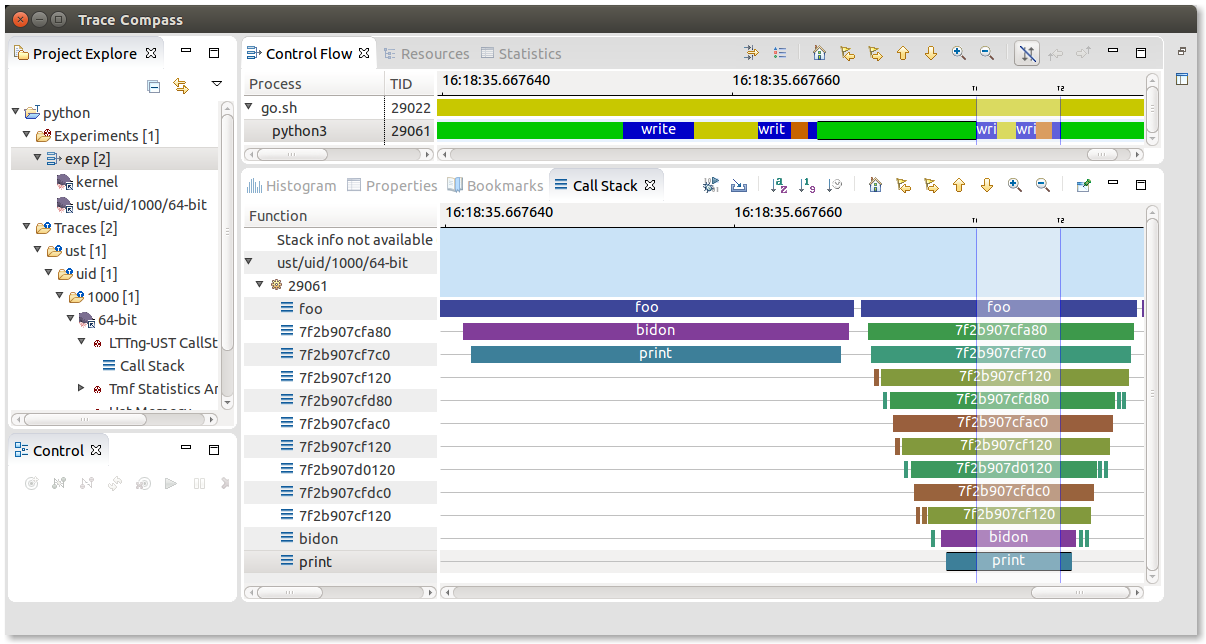
\includegraphics[width=0.90\textwidth]{figures/python-profile-ust-with-kernel.png}
            \label{fig:TraceCompass}
    \end{figure}
    
 
Focusing in real parallelism libraries, the tool Paraver \cite{paraver} is a visualization tool developed by the Barcelona Supercomputing Center. This tool currently traces MPI, OpenMP, pthreads, OmpSs and CUDA. It can be understood as a data browser of parallel traces. In this tool the metrics are programmed, computed from a series of functions and modules. The interesting aspect of  these tools, besides the real parallel traces analysis is the possibility to use programmable definitions to gather the metrics.\\
\subsection{Flame Diagrams}
Another important visualization method, is the Flame Graphs deveped by \cite{brendan_flamegraph}, which is able to show cpu resources and complements heat maps and icicle plots. Flame Graphs are not a tool specifically but rather a methodology of comparison of differences on hot paths in CPU profiling. They can be generated from several ways and originally focused in CPU profiling through linux perf\textunderscore events and might be used to find specifically the function that differ in terms of duration.\\
The tools arrived from the limitations of comparing several CPU profiling the normal tracing and profilers, where those tools could only represent with many lines of text the CPU profiling mechanisms.
Flame Graphs can be used to solve problems such as comparing MySQL data and CPU profiling applications. However, Flame Graphs can face some issues related to incomplete stack traces, function names missing. The incomplete stack traces may lead to incomplete conclusions.\\
A specific kind of Flame Graph, called Differential Flame Graph, DFG’s, is able to compare two flames by using a Red and Green scheme. The original Differential Flame Graphs can challenges in the ambiguity of the color scheme, which has two colors only: Green and Red. This kind of flame graph is used specific to highlight differences in two executions and find bottlenecks in functions of a program's call stack. \\
This methodology requires the full stack trace and consequently some tools might not provide all this information, the stack might also be incomplete or without the symbols loaded. In both cases the stack will be partially reproduced.
 
 \begin{figure}[h]
          \center
          \caption{Flame Graph}
            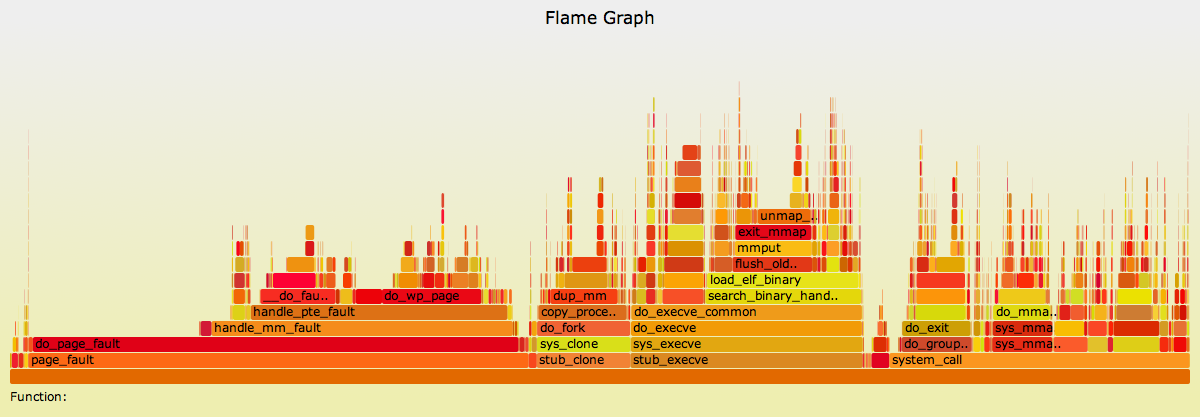
\includegraphics[width=0.90\textwidth]{figures/cpu-linux-execs.png}
            \label{fig:FlameGraph}
    \end{figure}
 
\subsection{Graphs}
In \cite{trevis}, a tool called Trevis, which is a visualization tool related to the calling context tree analysis is presented. It is a visualization and also an analysis framework with a different visualization pattern. It was developed to study the CCT produced from another tool called FlyBy software. It also, as TraceCompare, relies on a calling context tree, CCT, on the caller-callee relationship.\\

Trevis is a visualization and analysis framework that includes several visualization tools such as radial display, TreeMapRenderer, linear  and highrise renderer.
This tool allows the users to play with the Calling Context Trees and applying several methods to compare them. Trevis is able to compare the nodes using many metrics, such as Tree Edit Distance and Multiset Tree Distance. A dissimilarity matrix can be created to compare the similarities of the CCTs and clustering methods can be applied.\\
However, this tool relies in a human interaction and knowledge. Trevis relies on the data from FlyBy profiler tool, to stipulate on the slower executions. FlyBy provides after an report of failure containing this information that later can be used in Trevis to be analyzed.

\begin{figure}[h]
          \center
          \caption{Radial view in Trevis}
            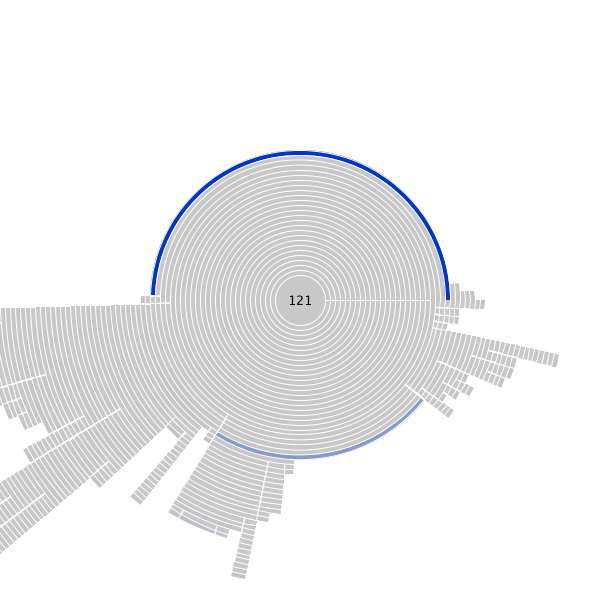
\includegraphics[width=0.60\textwidth]{figures/ring-600-color.png}
            \label{fig:RadialView}
\end{figure}
    
 
\section{Trace Correlation}
Trace correlation has appeared in the literature combining trace from userspace and kernel space. The work of Fournier et al., combines userspace and kernel space data aiming to analyse complex programs in high-level languages, that require userspace tracing, are often written in high-level languages but this work expresses the restriction of availability of those languages. This strategy can be used to compare and find specific differences in the traces aiming to extract more information than just one trace might produce. This is interesting taking in consideration that by using LTTng it is possible to trace them both.\\
In the work of \cite{pattern_based}, a solution that does trace correlation using patterns is used to compare different versions of the same software. The tracers of different versions are compared using a correlation metric, calculated in two approaches. First a non weighted approach, called NW\textunderscore TCM and a weighted approach  W\textunderscore TCM. The solution is composed of two phases, the pre-processing and the correlation calculation, using the already mentioned functions. The work is applied in the Weka \cite{weka} software and was able to correlate the versions 3.4 and 3.7 and found a 70 percent of dissimilarity. However, this technique does not necessarily is easily reproducible since the results require a synchronization mechanism with userspace and kernel space traces\\
Finally, in \cite{thomas}, this technique was also explored for embedded systems, specifically heterogeneous embedded, such as bare-metal CPU. In this work is introduced bare-ctf and it is used traces synchronization techniques. Indeed the solution is applied in Adaptiva Board and presents a generic solution to bare-metal system.
\section{Trace Comparison}
Several tools use the concept of trace comparison to obtain relevant information from the trace data and improve the performance software in general. We highlight here, three of those tools specifically focusing in the the problem definition.\\
One of those tools is TraceDiff\cite{trace_diff}, which does a comparison in the tracing by highlighting their differences. TraceDiff Compares  two  trace files and prints the details of packets that differ to standard output. This is useful for finding packets that are  present  in one trace but not another or for finding conversion or snapping errors. This tools relies in three main characteristic: scalability, robustness and ease of use. \\
However, as the other tools explained above, this tool requires the manual selection of the comparison traces and the analysis of their differences in visual aspects, since it shows the differences visually. The similar traces will be highlighted and connected, whereas the ones diferent will not be in this manner. \\
TraceCompare, was developed in Dorsal lab, \cite{tracecompare}, and it is a tool for performance comparison, it can be used in the two domains: userspace and kernel space. 
The methodology used in this tool is to create a tree data structure, a Calling Context Tree with metrics, from the tracing data to measure the executions of a program and that can have metrics. The segments are defined by the user as sequences of beginning and end, which will delimit the nodes in the tree data structure. The nodes also can aggregate data of the performance in those segments. \\
This tool was developed to compare traces of execution and it uses a javascript front-end and tibeebeetle as back-end. To do this CPU profiling comparison, the GUI tools provide Differential flame graphs, similar to  \cite{differential_flame}. It was able to find abnormalities in the write function of MongoDB after several runs. \\
However, TraceCompare requires expert knowledge and consequently, even after a statically tracing implementation the comprehension of metrics, as suggested in future work, \cite{doray_thesis}. Also the comparison is restricted to two groups and it is manually done. This last characteristic gives an interesting opportunity for further tools, such as our solution. 
\section{Root cause analysis and detection}
In terms of performance anomaly detection and bottleneck identification, PADBI, there is an interesting research currently with some trends. Part of the research is relative to the detection methods, while the other part concerns the identification of root causes, \cite{Chandola2009ADS15418801541882}.\\
In terms of anomaly detection the methods can be defined as detection of monitoring and might or not use data mining techniques. \\
The work of \cite{lasso} presents a Regression-based diagnostic framework for analyzing performance anomalies and potential causes of SLA violations in virtualized systems. Their approach is based in a variant of Least Angle Regression (LAR) called on Lasso, used to identify suspicious system metrics accounting for observed performance anomaly.\\
Another research, \cite{anomaly_detection_grid}, does models the relationship between application metrics and system metrics to explore properties of selection, reduction, and anomaly detection. The approach used combines the use of Fourier transform method, which will provide data to a windows averaging statistical. The use of the Fourier transform is to track patterns in the data.
In terms of root causes analysis several methodologies have been applied to this process. The terms analysis is related to the fact that those tools find the cause of issues.
Using kernel information, the work of \cite{tipme} investigates causes of unexpected long delays in GUI-based user interaction applications. This work developed the collection of tools called TIPME, The Interactive Performance Monitoring Environment. \\
The tool CloudPD,from \cite{cloudPD}, is an example of framework that uses linear correlation analysis to determine variations in Virtual Machines with uses cases like Hadoop and RUBiS. In this work there are several contributions specially in terms of implementation. In terms of root cause analysis the use of correlation-based performance models can be highlighted, although a similar approach was used in \cite{model_prob}.\\
The work of \cite{root_cause} detect anomalies in web applications using an approach called AOP-based monitoring, since it is based in Aspect Oriented Programming. It uses a correlation approach and time-series alignment to verify  the what is the root cause. The root cause analysis is done through a module called Performance Analyzer. This model applies an equation procedure and statistical correlation was done via three correlation methods: pearson correlation, Kendall rank correlation and Spearman Correlation, where the Pearson correlation gave the best results., which requires an alignment using Dynamic-Time Warping algorithm, DTW.\\
\section{Regressions Tests}
Regression testing is performed after making a functional improvement or repair to a program. Its purpose is to determine whether the change has regressed other aspects of the program, such as the performance, \cite{book_testing}. It can also seen as a confidence test proven that the new version works as the previous version\\
The importance of this kind of test is the tendency of adding bug codes throughout the development of updates. It is necessary to do a plan for regression test and before the release of the software, avoiding the deployment of bug code for users.\\
In terms of research at this topic, comparing releases, the work of \cite{parcs}, which developed the tool PARCS, does an investigation in regression tests using CCTs and matching techniques and bytecode comparison. The regressions are done using Apache Byte Code Engineering Library, BCEL. \\
Although not related to performance analysis, in \cite{book_testing}, it is addressed the problem of regression tests in objected oriented code using a comparison of interprocedural control flow graph, ICFG. This paper concerns the test selection problem specific for C++ languages providing a code based technique to in terms of test in the derived class.
\section{Dynamic Data Structures}
In dynamic analysis several data structures have been used to represent the call-caller relationship. The profile data can be either used for code optimization or for general program understanding. The organization of the procedures and its order usually are represented in a call graph or a calling context tree.
The call graph is a useful data representation for control and data flow programs which investigates interprocedural communication (i.e., how procedures exchange information). It contains all the procedures and the relationships among the procedures in a program. A call graph can be represented as a node as functions and edges as call-caller relationships. 
Taking in consideration the context, i.e. the chain of methods up to the root, two main methods are used: Call Trees and CCTs.\\
In the Call Trees, there is an addition of a new node is added for each called method. \\
This data structure can represent with accuracy the complete chain of methods of an application. \\
The other run time structure, calling context tree, CCT, provides flow sensitive profiling data with the nodes was introduced in \cite{blueprint}. In this work the hardware performance metrics from profiling were also taken in consideration in this work. Calling contexts are very important for a wide range of applications such as profiling, debugging, and event logging.  In \cite{blueprint} it is used a call graph to compare executions and explores the so called  performance evolution blueprint.  It is used to track the behaviour evolution of the system.\\
Following the previous work and by using tracing data, in \cite{doray_article}, aggregated performance metrics in a calling context tree to build an enhanced structure that could be compared. In this work it is built a tree with aggregated data, called ECCT, that relates the performance metrics to each node, which represents the functions of the application. This data is later analyzed off-line and, by using the critical path of the task, is able to find differences in the metrics of the ECCTs.\\
In the tool Introperf, \cite{Introperf}, the system stack traces is used to generate a specific CCT, which are called Performance Annotated CCT. In this tree a comparison technique is used to compare the latencies. It was implemented using Windows ETW,developed by \cite{ETW}. In terms of performance root cause, it is explained in the paper about the latency inference algorithm used for this calculation. They used this approach to avoid the requirement of source code or modification to application.\\
Another tool that builds CCTs is PerfDiff, which targets VM’s \cite{perfdiff}. In this work a framework for characteristics of those trees. According to the authors, it is possible to compare the CCT’s in two complementary ways: weight difference and topological difference. The first kind of comparison is the weight difference that is done in two ways: node based weight matching and sub-tree base weight matching. The topological differences are done via common tree matching, which is an algorithm developed by them which states that the nodes match (of each tree) when all the nodes in the path from the root match. This approach is applied to several Java and J2EE applications where the call counter are used as performance attributes.\\
In terms of building the CCT, two main techniques were used previously to collect the stack frames of the application, in the so called stack walking process. The exhaustive approach and the sampling based approach, although other methods such as static and adaptive bursting had been used.\\
When taking all the tracing entries and exists to build the CCT, the result will be the complete tree of the application. The overhead of adding all the entries and exits is a major drawback in this approach.\\
The second main approach is the sampled technique. This technique is able to reduce the overhead in comparison with the exhaustive but has two main disadvantages: inference of calls, which may lead to misinformation and the rate of sampling may not be feasible to a certain extend.\\
Other approaches are possible such as static stack walking and adaptive stack walking. The same authors of PerfDiff, previously proposed the use of Adaptative Bursting technique for the stack walking process in \cite{adaptative_burst}. This kind of stack mechanism avoids the overhead of creating the trees in a process of eliminating certain profile data redundancies.
We also used a version not summarized of the frames with the metrics, and in analogy to the ECCT, the tree was named EDT, Enhanced Dynamic Tree. They are very similar, though the EDT is not summarized and can facilitate the mining process relating each node to the metrics without further calculus. 
\section{Auto Grouping mechanism}
During software execution several parameters might change and the application performance can vary according to many factors. This can occur even when the algorithms used are deterministic and no probability is used. The cause for those variance are outside the scope of the program itself.
However, some applications might have issues in the code, related to its implementation details. Software tests mechanisms might not be sufficient to reveal this behavior especially in terms of performance discrepancies.\\
An example was found in \cite{doray_article}, after executing several times the same query operation on MongoDB, a free open-source database framework, its performance decreases abruptly a further investigation lead to the root cause of this performance issue. \\
The auto grouping technique presented as the solution for those kinds of problem. The approach is to do automatic comparison of executions of the same program in the same configuration settings and investigate their metrics behavior. \\
The solution is automated by a heuristic comparison of several groups distributions and can be applied to an arbitrary number of groups together with a clustering mechanism, such as k-means. The automatic grouping gives the optimal number of groups in terms of SSE and together with a comparative mechanism, can be used to find associations between groups. 
The division in groups enables the comparison and study of their variances using different approaches, for a few number of groups the investigation by the comparison the variances of the metrics of the groups can lead to the discovery of root causes. Another approach can be the use of apriori algorithm which can be applied to find association among the groups. 
The complete solution is able to find associations between the performance and metric variations, i.e. groups of different performances and metrics. This can indicate if a specific metric is responsible for a certain groups of execution that have a bad performance, in a fuzzy approach and that can be applied for infrequent problems.\\
\section{Conclusion of the Literature Review}
In terms of dynamic analysis of an application, tracers, profilers and debuggers can be used, each one with its own specific pros and cons.
Profilers represent the caller-call relationship and allows a deep understanding of the time consumed in an application. Profilers add extra overhead and might not be suitable to find performance issues that occur in group in several execution of software.\\
Debuggers can be used specifically to find a part of code that might trigger issues in the execution. This tool relies in breakpoints that will stop the execution in a specific condition. This process allows specific conditions in the source code to be tests and bug finding and fixing accessible. \\
Finally, tracers use advanced technologies and implementations to record events occurring at several levels in a computer system with minimal overhead. This feature makes tracing a useful mechanism to understand and analyze the behavior of the system in the real context.\\
By using tracing technique it is possible to develop a data structure which represents the dynamic execution of a system but also can be embedded with performance data recorded in the tracing data. Several other techniques can relate this performance data with specific functions in the same node and allows associations of metrics and functions.
In summary, several strategies make it possible to extract from one or more traces all the events related to a given task execution. However, there is a demand for automated tools to analyze the performance.  \\
This research is based on the several methods of comparing performance data that were introduced in this chapter, including data mining technique and statistical evaluations gathered using profiling and tracing mechanisms. In the next chapter, we present the methodology used throughout our solution.\\

\section{Summary of the tools}
The table \ref{tab:tableComparative} summarizes part of the related research.\\

 \begin{table}[h]
\centering
\caption{Table Comparative tools for performance analysis}
\label{tab:tableComparative}
\resizebox{1.1\textwidth}{!}{%
\begin{tabular}{lllll}
\hline
Tool             &    Intention & Pros & Cons & Kind of tool   \\ \hline
PerfDiff &  Generate CCT in VM’s & Node and weight comparison & Topological differences might mislead & Detection and analysis \\
\hline
TraceCompare & Compare groups of executions & Easy to use  & Manual select entries and exits & Detection and analysis\\ \hline
Spectroscope & Distributed system behaviour categorization & Automated k-means & -Time for the analysis -Relies in end-to-end instrumentation  & Detection Analysis\\\hline
Introperf &  Generate CCT & Based in ETW  & -Complete stack walking -overhead & Detection and analysis
\\ \hline
 
Spectraperf \cite{SPECTRAPERF} &  Detection of I/O regressions & Efficient performance Specific for I/O &  Comparison of two software versions & Detection and analysis
\\ \hline
Pinpoint &  Build runtime paths on large systems & Comparison using a free context grammar & ANOVA requires normal distributed data & Detection and analysis\\ \hline
TraceCompass &  Trace Analyze &  Several internal tools and methods & Manual analysis & Analysis \\ \hline 
Magpie & Automatic tool chain builder & Use of a comparative metric: string-edit-distance metric & Probabilistic construction of the event & Detection and analysis\\ \hline 
Trevis &  CCT analysis tool & Manual method & Rely in another tool & Visual method Analysis 
\end{tabular}
}
\end{table}

  % Revue de littérature.
\Chapter{METHODOLOGY}\label{sec:Theme1}
In this chapter the problem, research assumptions and research questions will be stated.
\section{Problem Definition}
The problem addressed in the work can be summarized in comparing several times the executions of software have different performances for several factors, intrinsic and extrinsic of the program itself.
\section{Research assumptions}
(i) It is possible to gather information from tracing records and understand it using high level abstractions and data structures.\\
(ii) It is possible to associate and/or correlate metrics gather from traces using mathematical techniques in a meaningful way.\\
(iii) The difference among the groups will give an indication of the performance issue, i.e. association is an indicative of causality\\
It is also important to highlight that this work partially relies on previous works (i) \cite{doray_thesis}.

\section{Research Questions}
\textit{Is it possible, using high level abstractions and dynamic data structures, to find root causes for performance differences?}\\
\textit{Minor question: What are the limitations of the current techniques?}\\
  
Although most of the time for performance analysis a visualization tool is used, quite often is mandatory specialized knowledge to interpret the information gathered to solve real problems. On real situations moreover, it is required time to analyze and solve a problem, so a more automatic approach can be taken on those cases. To interpret the information from traces in a meaningful way, it will be necessary to do some correlations and use more high level abstractions than just comparing traces.

\section{Specific objectives}
The aim of this research is to aim for an automation of trace analysis and several mechanisms are explored on that direction. From this objective, we were able to develop this was helpful to identify precisely the root cause of performance bottlenecks on software applications.\\
The field of tracing tools is very specific and relies on analyzing a considerable amount of information from the trace files. In fact, just some few seconds of recording can give an enormous amount of information to be analyzed. Therefore, there is a tool dependency for generating this information, but also a knowledge dependency, since the interpretation of this data depends on performance analysts.  

\section{Solution Design}
The design of the solution was developed to target two specific aspects: automation and flexibility. 
The first automation, is that the solution can be applied with minimal intervention. That is, it can be used without a specific pre-phase of the learning and labeling the data. The presented solution is complementary to some techniques of clustering, such as k-means, requires the number of k, i.e. the number of groups.\\
The second is that the flexibility of this approach, that can be used with different grouping and clustering techniques. The heuristic comparison possibilities the use of many clustering and grouping mechanisms such as k-means algorithm.\\
As trade-off of the approach, the time increased since the heuristic comparison applies several times the execution of clustering methods.
\section{Approach}
The approach used for the solution can be divided in two parts: the data collection tools and the data analysis methods, presented below respectively:
\subsection{Data collection tools}
The tools used for data collection were LTTng and Perf counters. The applications were statically instrumented or compiled with the instrumentation. LTTng provides a small overhead, so the traced application can run with a negligible performance difference. Perf is able to provide the hardware and software performance counters for the executions.
The tracing of the executions will provide the data that later will be used for the construction of the tree, i.e. ECCT or a EDT, Enhanced Dynamic Tree.
\subsection{Data analysis methods}
In terms of data analysis several methods were applied, for example: k-means, percentage classification and Support Vector Machine. Later it was applied the auto grouping technique above all previous ones to automate them.\\
The first method, k-means, is a centroid algorithm which does the optimal grouping data. This algorithm will guarantee the best partitioning of the data with an specific k, the k is the number of groups and must be given a priori.\\
The second technique, percentage classification is a method of grouping a percentage of distance near the points, similar to a range classification. Several percentages can be tested to reduce or enlarge the distance.\\
The auto grouping technique, using heuristic classification, was used later developed to fulfill the need for an automated flexible classification mechani. The mechanism is composed basically of comparing a statistical measurement of deviations within the groups called SSE. This technique is able to find groups automatically since they SSE has a interesting behavior that can be tracked using the so called elbow heuristic, this enables the comparison of several SSE of different groups and the finding of the optimal value for grouping. The heuristic does not required to be a pre-classification.
\subsection{Testing Framework}
For the testing settings we developed a testing framework in C++ using the QtCreator Framework. The framework was used to test the concept of the models and grouping techniques by simulating a series of specific performance issues that are measured by perf counters.\\
In those specific scenarios, such as high cache-misses or page-faults, the measurements were made in such a way that they are later exported to a comma-separated-value file, CSV file.
\section{Solution Application}
The solution can be applied to several scenarios where the performance counters are able to measure the real behavior of the system and the tracing data has minimal or negligible influence in the real program.
An interesting application of the solution are regression tests, which aim for finding performance regression in one version to another. Indeed the solution can be integrated as it is in test sets aiming to find the performance issues before the deployment of the application.
\section{Co-authored articles}
In partnership in \cite{google_releases} we did performance measurements using Confidence Interval. This work was accepted at the conference QRS 2017, we applied a comparative technique data from Google Chrome performance measurements. The challenge was to detect performance deviations among Chromium software releases. The method done was to compare the confidence interval, using the median instead of the mean, as mean of comparing several releases.\\
As result, we were able to demonstrate that this method of confidence interval, using medians, is able to compare the releases similarly to a t-test and was able to determine performance deviations at a function-level granularity with a small number of trace samples.\\
Although the ground truth is still required the method showed a better performance than the standard Confidence Interval, which consider only the mean. 
This method can be combined with a clustering technique to avoid (or at least reduce) the influence of outliers, which can difficult the analysis of comparative data. Another possibility of using clusters is to enhance the confidence of the comparative intervals.
\section{Authored articles}
The chapter 4, Articles, will explain with details the specificities of the article. This article presents our development of a solution to find root cause analysis automatically. 
The first step is to trace the application recording the performance counters, in the experiments this was done with LTTng and Perf. The second step is to execute the program several times and until enough data from the performance variations were found, the data is then recorded and a dynamic data structured with the tracing data and the performance counters is developed. Then, the third step is to run the analysis mechanism to group the data automatically. After the groups are segregated it is possible to compare their inner characteristics, that is it, the metrics recorded in the tracing. A statistical approach can be used to compare the groups directly but also a frequent mining association, such as the Apriori methodology, can be used to associate the groups as well.\\
The different tests show the flexibility of the model, which can be used in combination to a clustering or grouping mechanism for the  grouping division.
             % Premier thème (Doctorat) ou "Détails de la Solution" (Maîtrise).
\Chapter{ARTICLE 1: PERFORMANCE ANALYSIS USING AUTOMATIC GROUPING}\label{sec:Theme2}
\textbf{Authors}\\
Isnaldo Francisco de Melo Junior\\
École Polytechnique de Montréal\\
Isnaldo-francisco.de-melo-junior@polymtl.ca\\
 
Michel Dagenais\\
École Polytechnique de Montréal\\
michel.dagenais@polymtl.ca\\
 
\textbf{Index terms} – Performance analysis, Tracing, Software visualization, Heuristic, Groups.\\

\section{Abstract}
\label{sec:abstract}
Performance has become more important on software development and maintenance. To address this concern, teams of developers use tracing tools to improve the performance or track performance related bugs. On this work we developed an automated technique to find the cause of performance issues, which do not require deep knowledge of the system. This approach is capable to indicate the performance cause using a comparative methodology on slow and fast executions. We applied the solution on some use cases and were able to find the specific cause of them. Also, we implemented the solution on a framework to help developers on similar problems together with a differential flame graph tool.


\section{Introduction}
\label{sec:introduction}
Software performance is a major concern for software development. Various studies highlight the use of tools as debugging and tracing to help on performance problems, which can be used to improve performance or detect performance issues.
% The problem
One example of performance issue is the comparison of similar executions of the same program in the same configuration setting. An example was found in \cite{doray_article}, after executing several times the same query operation on MongoDB, a free open-source database framework, its performance decreases abruptly a further investigation lead to the root cause of this performance issue.

% The solutions
For this kind of performance problem, which is related with the execution inside a real system, the current solutions are to debug or to trace it. The first one, debugging, is the location of code and wrong executions directly on the source by execution the code in a locked environment using breakpoints. However, some debugging tools require the reproduction of the exactly issue to trigger the same code mechanism and its necessary to retard the execution of the program while doing this process.

On the other hand, a trace is an execution log of a software that consists essentially of an ordered list of events. An event is generated when a certain path of the code is executed, commonly denominated tracepoint, where each event consists of a timestamp, a type and some arbitrary payload \cite{francis1}. tracepoints can be embedded on the code in two ways: statically or dynamically inserted. The later, dynamic tracing, gives the possibility to add tracepoints without modifying the source code and the sooner requires the modification of the source code. Besides, tracing can be performed at the kernel and user-space level \cite{francis1}.\\

Unlike debugging, it is possible to trace a program without interrupt it, yet, there is an overhead caused by its usage. A good tracer needs to minimize the disturbance of the running program to be a useful tool for analysis. LTTng\cite{desnoyers}, developed by Mathieu Desnoyers, has this minimal level of impact on the system and consequently allows to trace the user-space and the kernel space with minimal interference. LTTng, allows the analysis of task interactions with each other and with the operating system. Locating and analyzing performance problems is not a trivial activity because of their large size, since more events generate more information to be gathered and analyzed. 

After collecting the data on the tracer, it is necessary to analyze the software behaviour through some mechanism, for instance the call graph \cite{call_graph}. A call graph is a representation of the stack frames of the software and can be built using different techniques. This analysis requires expert knowledge and deep analysis of the system since this process was not automated yet.

Through tracing mechanisms is possible to build a dynamic model of the software or, in other words, a calling tree of it. Moreover, tracing allows the possibility to add performance measurements to this structure, as shown in \cite{doray_article}.

In summary, from the enhanced data structure described above and considering the lack of an automate solution to solve problems as the stated above, it is possible to build a solution that records several software properties at run time. Moreover, using some specific grouping mechanisms it is possible to find root causes of several performance issues using this comparative approach.\\

This paper introduces an automated solution for clustering metrics using the call context tree to find performance related issues. We implemented it on TraceCompass with visualization mechanisms to facilitate the analysis of different aspects of the Calling Context Tree. Then we applied this technique on four different use cases to analyze the performance problem of them. Finally, we discuss the drawbacks of this technique and the possible solutions to overcome them aiming to apply this analysis on real software.

The research aims to investigate the following research questions;

\begin{itemize}
\item RQ 1: How can we build an efficient and flexible model for performance comparison?
\item RQ 2: How to automate the performance analysis on several runs using performance counters?
% \item RQ 3: The root cause found using the approach is accurate?
\item RQ 3: How accurate was the obtained results ?
\end{itemize}

\textbf{This paper is organized as follows} The related work is presented in section \ref{sec:related-work}, then the solution is presented in \ref{sec:solution} with the clustering technique. In section \ref{sec:methodology}, we present the methodology used followed by the micro-benchmarks and an illustrative example of the analysis. The use case section \ref{sec:usecases}, the discussion of the results \ref{sec:results} and a section with some limitations \ref{sec:validity}. Finally the conclusion \ref{sec:conclusion},

 
\section{Related Work}
\label{sec:related-work}

%Specifically considering the approach used here, comparing the metrics of a program to classify them the work of Francois Doray, in TraceCompare has a similar approach.
In this section will be presented the basic principles of current tools used to find performance issues. The related work was divided in: Data collection, Analysis tools and Visualization tools that are described below.\\

% \textbf{Data collection}\\
From the perspectives of Data Collection, there are two main works related to this work, LTTng and Linux Perf Events.

% \subsection{LTTng}
The first, LTTng, Linux Trace Toolkit Next Generation \cite{desnoyers}, tracer can record events from the Linux kernel and from user space applications into a single trace. It is also designed to have a minimal overhead on traced systems. It is therefore well suited to our goal of collecting all the factors that contribute to the execution time of tasks in production environment.\\

% \subsection{Linux Perf}
The second, Linux Perf Events is a profiler tool for Linux 2.6+ based systems that abstracts away CPU hardware differences in Linux performance measurements and presents a simple command-line interface. Perf is based on the perf events interface exported by recent versions of the Linux kernel. This article demonstrates the perf tool through example runs \cite{perf}. It is possible to record software events and hardware events \cite{vitillo}.\\
It is interesting to highlight that the Perf tool can be used to record profiles on per-thread, per-process and per-cpu basis \cite{perftool}.\\
% \textbf{Analysis tools}\\
From the point of view of Analysis tool, there are two main tools related to this work, TraceCompare and Trevis.
% \subsection{TraceCompare}
The first tool, TraceCompare, was developed in Dorsal lab \cite{tracecompare}, which creates an enhanced Calling Context Tree to measure the metrics from specific segments of a trace. Those segments are defined by the user as sequences of begin and end. This tool was developed to compare traces of execution and it uses a javascript front-end and tibeebeetles as back-end. To do this CPU profiling comparison, the GUI tools provides a Differential flame graphs as defined in \cite{differential_flame}.
 It was able to find abnormalities in the write function of MongoDB after several runs. However, TraceCompare requires expert knowledge and also some statically metrics of analysis \cite{doray_thesis}.\\
% \subsection{Trevis}
The second tool, from Lugano University, Trevis \cite{trevis}, is a visualization and also an analysis framework. It was developed to study the CCT produced another tool called FlyBy software. Like TraceCompare, it relies on a calling context tree, CCT, on the caller-callee relationship. Trevis is a visualization and analysis framework that 
allows the users to play with the CCTs by applying several methods.
However, this tool relies in a human interaction, which occurs at FlyBy, to stipulate on the slower executions. FlyBy provides after an report of failure containing this information that later can be used in Trevis to be analyzed.\\
% \subsection{Spectroscope}
The third tool, Spectroscope, was developed in \cite{Sambasivan2011DPC19724571972463}, that is a tool that uses statistical and high level analysis, in fact, it was design to find changes in behaviour, not find specific anomalies and it was used to find problems in two versions (or periods) on Google's Ursa Minor distributed software. Specifically for this software, five problems are described. It uses Startdust as end-to-end tracers and it added some overhead on Ursa Minor performance, depending the operation. \\
It uses Perl language and MATLAB statistical comparison of no problematic period and a problematic period, also using DOT for the plotting part.
The statical comparison used is the Kolomogrov-Smirnov test,  which is a non-parametric test for mutation identification that compares the shapes and distribution of mathematical function and later using a ranking system for mutation identification.\\
 Spectroscope uses normalized discounted cumulative gain (NDCG), for the performance evaluation is used a range evaluation. Spectroscope is similar with Pip in \cite{Pip} and TAU in \cite{TAU}.\\
% \subsection{Introperf}
Finally, Introperf developed by \cite{Introperf} is a tool that uses system stack traces to generate CCT, called Performance Annotated CCT that they call PA-CCT. Then, it ranks the latencies and compare them \cite{Introperf}. The intend of this tool is to be used in a post-development stage. It was implemented using ETW, \cite{ETW}. It is explained on the paper about the latency inference algorithm used for this calculation. They used this approach to to avoid the requirement of source code or modification to application. \\

% \textbf{Visualization tools}\\
% \subsection{Flame Graph}
From the point of visualization of comparison technique, the flame graphs and differential flame graphs, developed by Brendan Gregg is a very popular technique. They can be used for comparing the executions, it is possible to use a Flame Graph diagram. As defined by Brendan Gregg \cite{differential_flame}, Differential Flame Graphs can be a useful tool for comparing executions. A Differential Flame Graph is a visualization technique highlight differences on collections of stack traces (aka call stacks), from two different executions. Flame graphs are commonly used to visualize CPU profiler output, where stack traces are collected using sampling.


\section{Motivation}
\label{sec:motivation}
The main motivation for this research was the current limitations of the current tools to track problems on executions that does not appear often, for example one execution long run among a thousand that work perfectly. 
This difficult relies mainly on the amount of data that is needed to be generated and analyzed comparatively. 

From the point of view of the grouping techniques, the current more reliable technique still require some human analysis of the data, which would consume time and undermine an automated technique. This is the reason for the development of the auto grouping technique, which combines an heuristic evaluation.


The implementation also developed the RGG differential flamegraph to compare groups of executions. This implementation uses a three colors: red, green and gray. This was necessary to avoid the ambiguity that the original work developed by Brendan Gregg gave, where the green color could mean faster execution or equal execution, in a comparative way.

This methodology developed can be applied in other scenarios and it is independent from the implementation. Besides it is also independent from the grouping algorithm, since it is an heuristic and not an algorithm. Combined with the Apriori algorithm, the grouping technique can provide strong insights on complex cases.

Finally the motivation to implement the solution in TraceCompass is because of its reliability as trace framework. TraceCompass is currently supported by Ericsson Inc. and Dorsal lab at Polytechnique Montreal, and has several features, which combined, form a complete analysis framework for different kinds of traces.

\section{Solution}
\label{sec:solution}
On this section, we discuss about the solution developed, starting from the data structure, which the work relies, then the algorithms used to do the grouping mechanism, then the cluster algorithm and the overall methodology. \\

  The methodology can be summarized in the following process:\\
  First, we trace a program using statically or dynamically embedded tracepoints. Then we read the tracing and develop a CCT recording, also the performance metrics. Later, we run the clustering techniques and the association rule, which indicated the possible cause of the performance issue.
  
    \subsubsection{Recording of execution}
    We record the program executing using LTTng, this tracer has low overhead, therefore is adequate for this type of research. 
    The trace is also recorded with the performance metrics such as instructions, cache-misses, page-faults, and schedule switches by using the perf counters tools in Linux.
    
    \subsubsection{Generating the data structure}
    After the recording in different scenarios, a pre-processing of building a structure for comparison is done, this structure is a enhanced calling context tree. 
    To do this process, we use trace compare to divide the tracing in segments, delimited using: e.g. in the case of sys\_open, we used systemCallOpen and systemCallExit.
    In this process we aim to construct comparable information using ECCT (or EDT), which each node represent a call and the information in this call will be within the nodes. A delta of the entry and the exit for each metric is recorded in the node, in a sampling scheme.
    
    \subsubsection{Clustering technique}
    After the data was pre-processed and the tree is built, a mathematical model is done and its behaviour compared to its input can be determined. 
    
    \subsubsection{Execution Comparison}
    With the groups divided the next phase is the comparison among them. There are possible to ways to compare the groups: compare the mean and median for each group or use the Apriori Association described in section \ref{sec:association}.
    
\subsection{Data Structure}
% \textit{Call Graph}\\
%     The call graph is a useful data representation for control and data flow programs which investigate interprocedural communication (i.e., how procedures exchange information). It contains all the relationships among the procedures in a program and can contain auxiliary information concerning the
%     data within each procedure and global data shared among procedures \cite{call_graph}.

\textit{Calling Context Tree}\\
Calling contexts are very important for a wide range of applications such as profiling, debugging, and event logging. Most applications perform expensive \textit{stack walking} to recover contexts\cite{precise}. The resulting contexts are often explicitly represented as a sequence of call sites and hence bulky. The goal of calling context encoding is to uniquely represent the current context of any execution point using a small number of integer identifiers (IDs). This data structure was introduced by \cite{27} and reused by \cite{4}, \cite{28}.
% \textit{Enhanced Calling Context Tree}\\
    In this work we aggregate data, related to the performance on the Calling Context Tree, which gives the concept of enhanced structure. The aggregated data is related with the performance metrics, the data is added in the tree nodes and gives the possibility to be analyzed off-line.
    The Figure \ref{fig:ecct_dt} demonstrates the difference between the dynamic tree and the calling context tree.
    \begin{figure}[h]
        \centering
        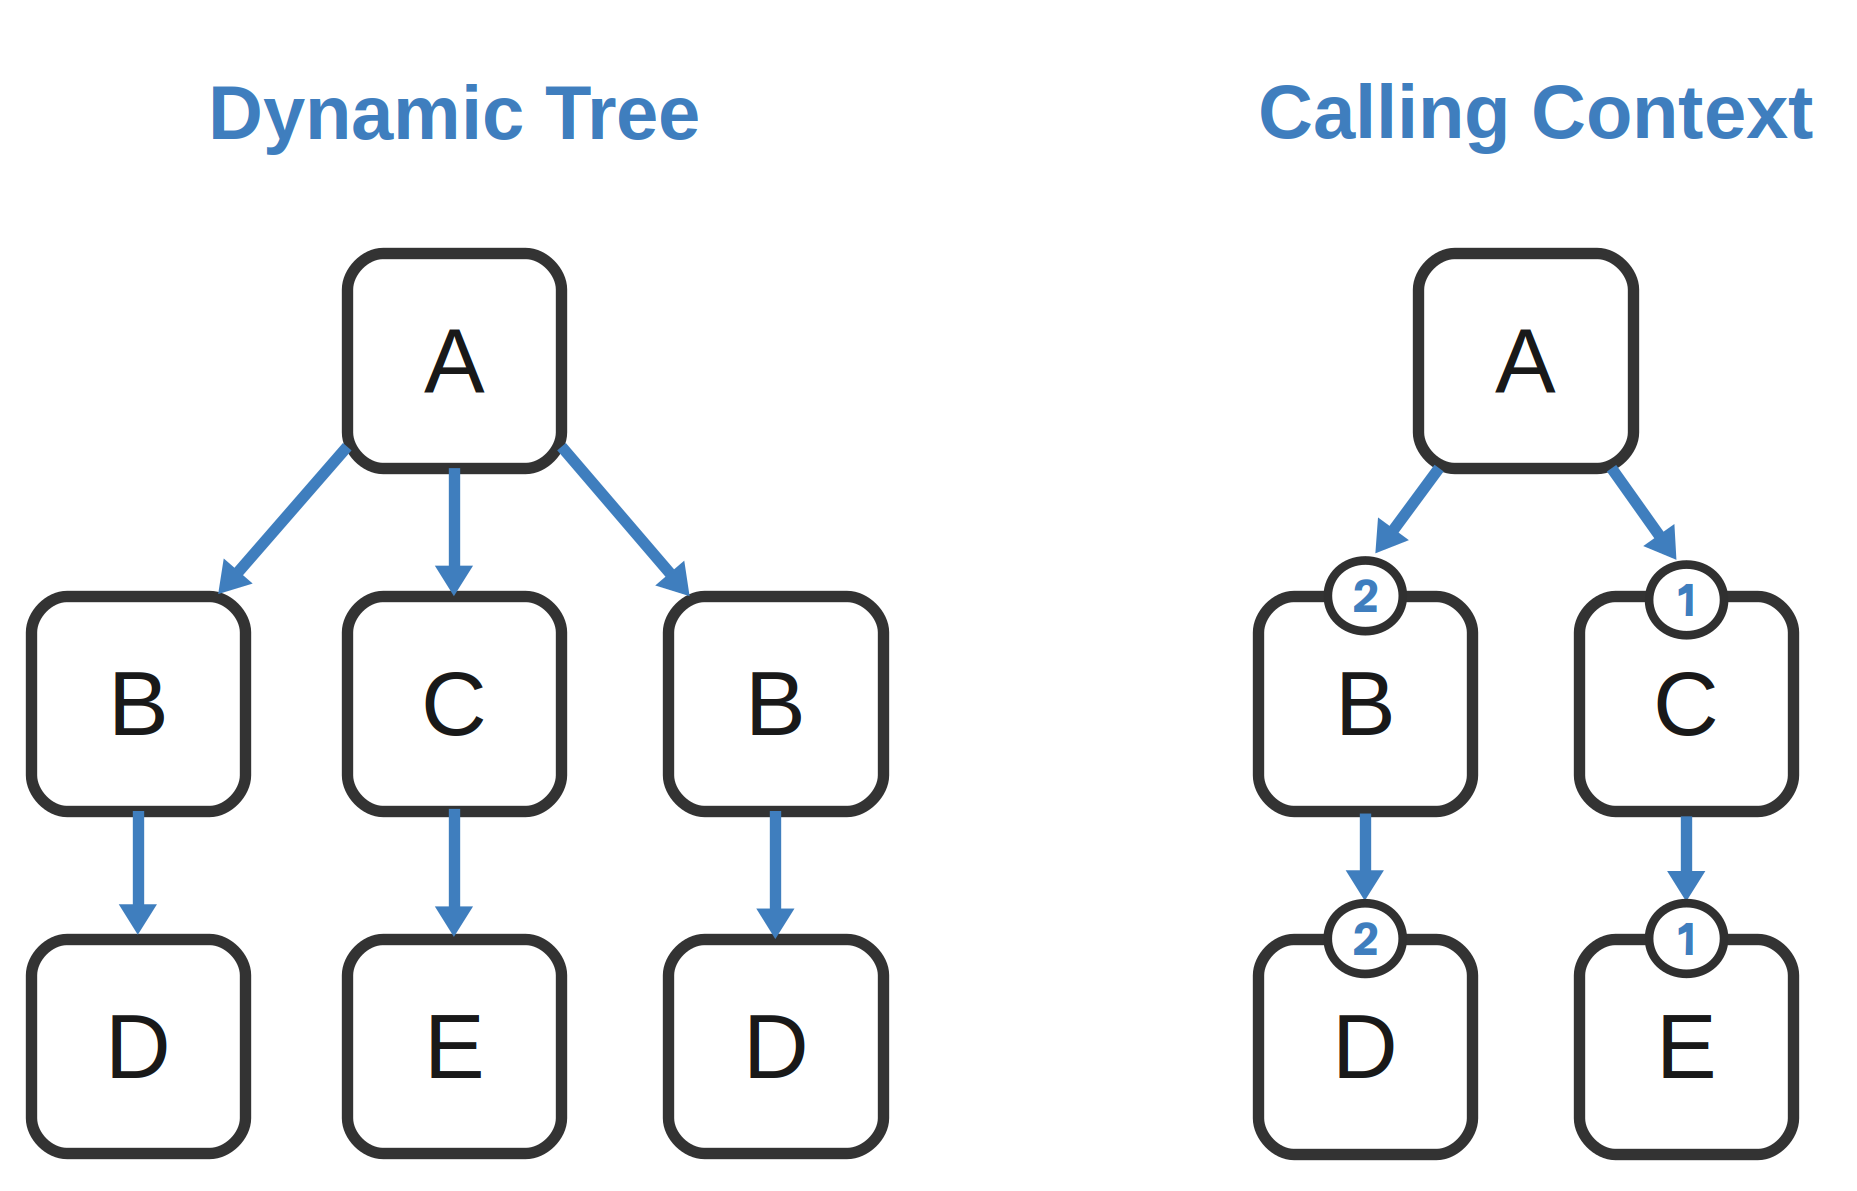
\includegraphics[width=0.40\textwidth]{figures/dynamic-calling.png}
        \caption{Dynamic Call Graph vs Enhanced Calling Context Tree }
        \label{fig:ecct_dt}
    \end{figure}
    The metrics recorded inside the tree are described in the subsection Performance Metrics.
    
\textit{Performance Metrics}\\
    In virtue of generating a tree through a tracing approach, it is possible to record runtime information of the system \cite{francis1}.
    They are recorded using the lttng feature add-context, and this gives the possibility to add performance counters in the tracing session.\\
    Example: perf:cache-misses, perf:major-faults, perf:branch-load-misses\\
    This technique was explored in the work of \cite{doray_thesis} and \cite{olsa}.
    Although we took several metrics in consideration, we summarizes three metrics before introduce the clustering mechanism.\\
    
%\textbf{cache-misses}\\ 
%       When a program accesses a memory location that is not in the cache, it is called a cache miss. Since the processor has to wait for the data to be fetched from the next cache level or from main memory before it can continue to execute, cache misses directly influence the performance of the application \cite{washington}.
%       The concept of cache miss ratio, is the ratio of memory accesses that cause a cache miss. From the miss ratio you can usually tell whether cache misses may be a performance problem in an application.
      
%\textbf{page-faults}\\
%       A page fault is the sequence of events occurring when a program attempts to access data (or code) that is in its address space, but is not currently located in the system's RAM. The operating system must handle page faults by somehow making the accessed data memory resident, allowing the program to continue operation as if the page fault had never occurred\cite{redhat}.
      
%\textbf{cpu instructions}\\ 
%       This metric is the measurement of the instructions related to arithmetic, logical and shift operations on values in registers. 
    
    
\subsection{Data Structure Construction}
    The construction of the ECCT involves the reading of the tracing in order and simultaneously building the nodes as soon as the data is coming. It is necessary to delimit the boundaries of the nodes in the tree. Therefore, to set events as starting and end points of the nodes. Depending on the case, the construction of the tree depending on the case might be easy to be done using a ECT, instead of ECCT.\\
    Consequently, it is necessary to demultiplex the events on the trace. To do so, the trace must provide a way to identify the start and end points of each execution. 
    For this process there are two approaches:\\
    First, use existing events of the Linux kernel. As an example, the syscall\_exit\_accept event (generated when a connection is accepted on a socket) and the syscall\_entry\_shutdown event (generated when a connection is closed) correctly delimit requests received by an Apache server. \\
    Second, is to use LTTng-UST probes, statically inserted in the source code. Different probe types can be used to delimit different execution types. In that way, the delimitation of the nodes can be done.
    An advantage the first approach is to use existing events and thus, no access to the source code is required. The advantages of the second is that no kernel knowledge is required to use this process.
    
    The Figure \ref{fig:ecct_build}, demonstrates the mechanism used to create the ECCT from the tracing file.
    
\begin{figure}[h]
      \centering
        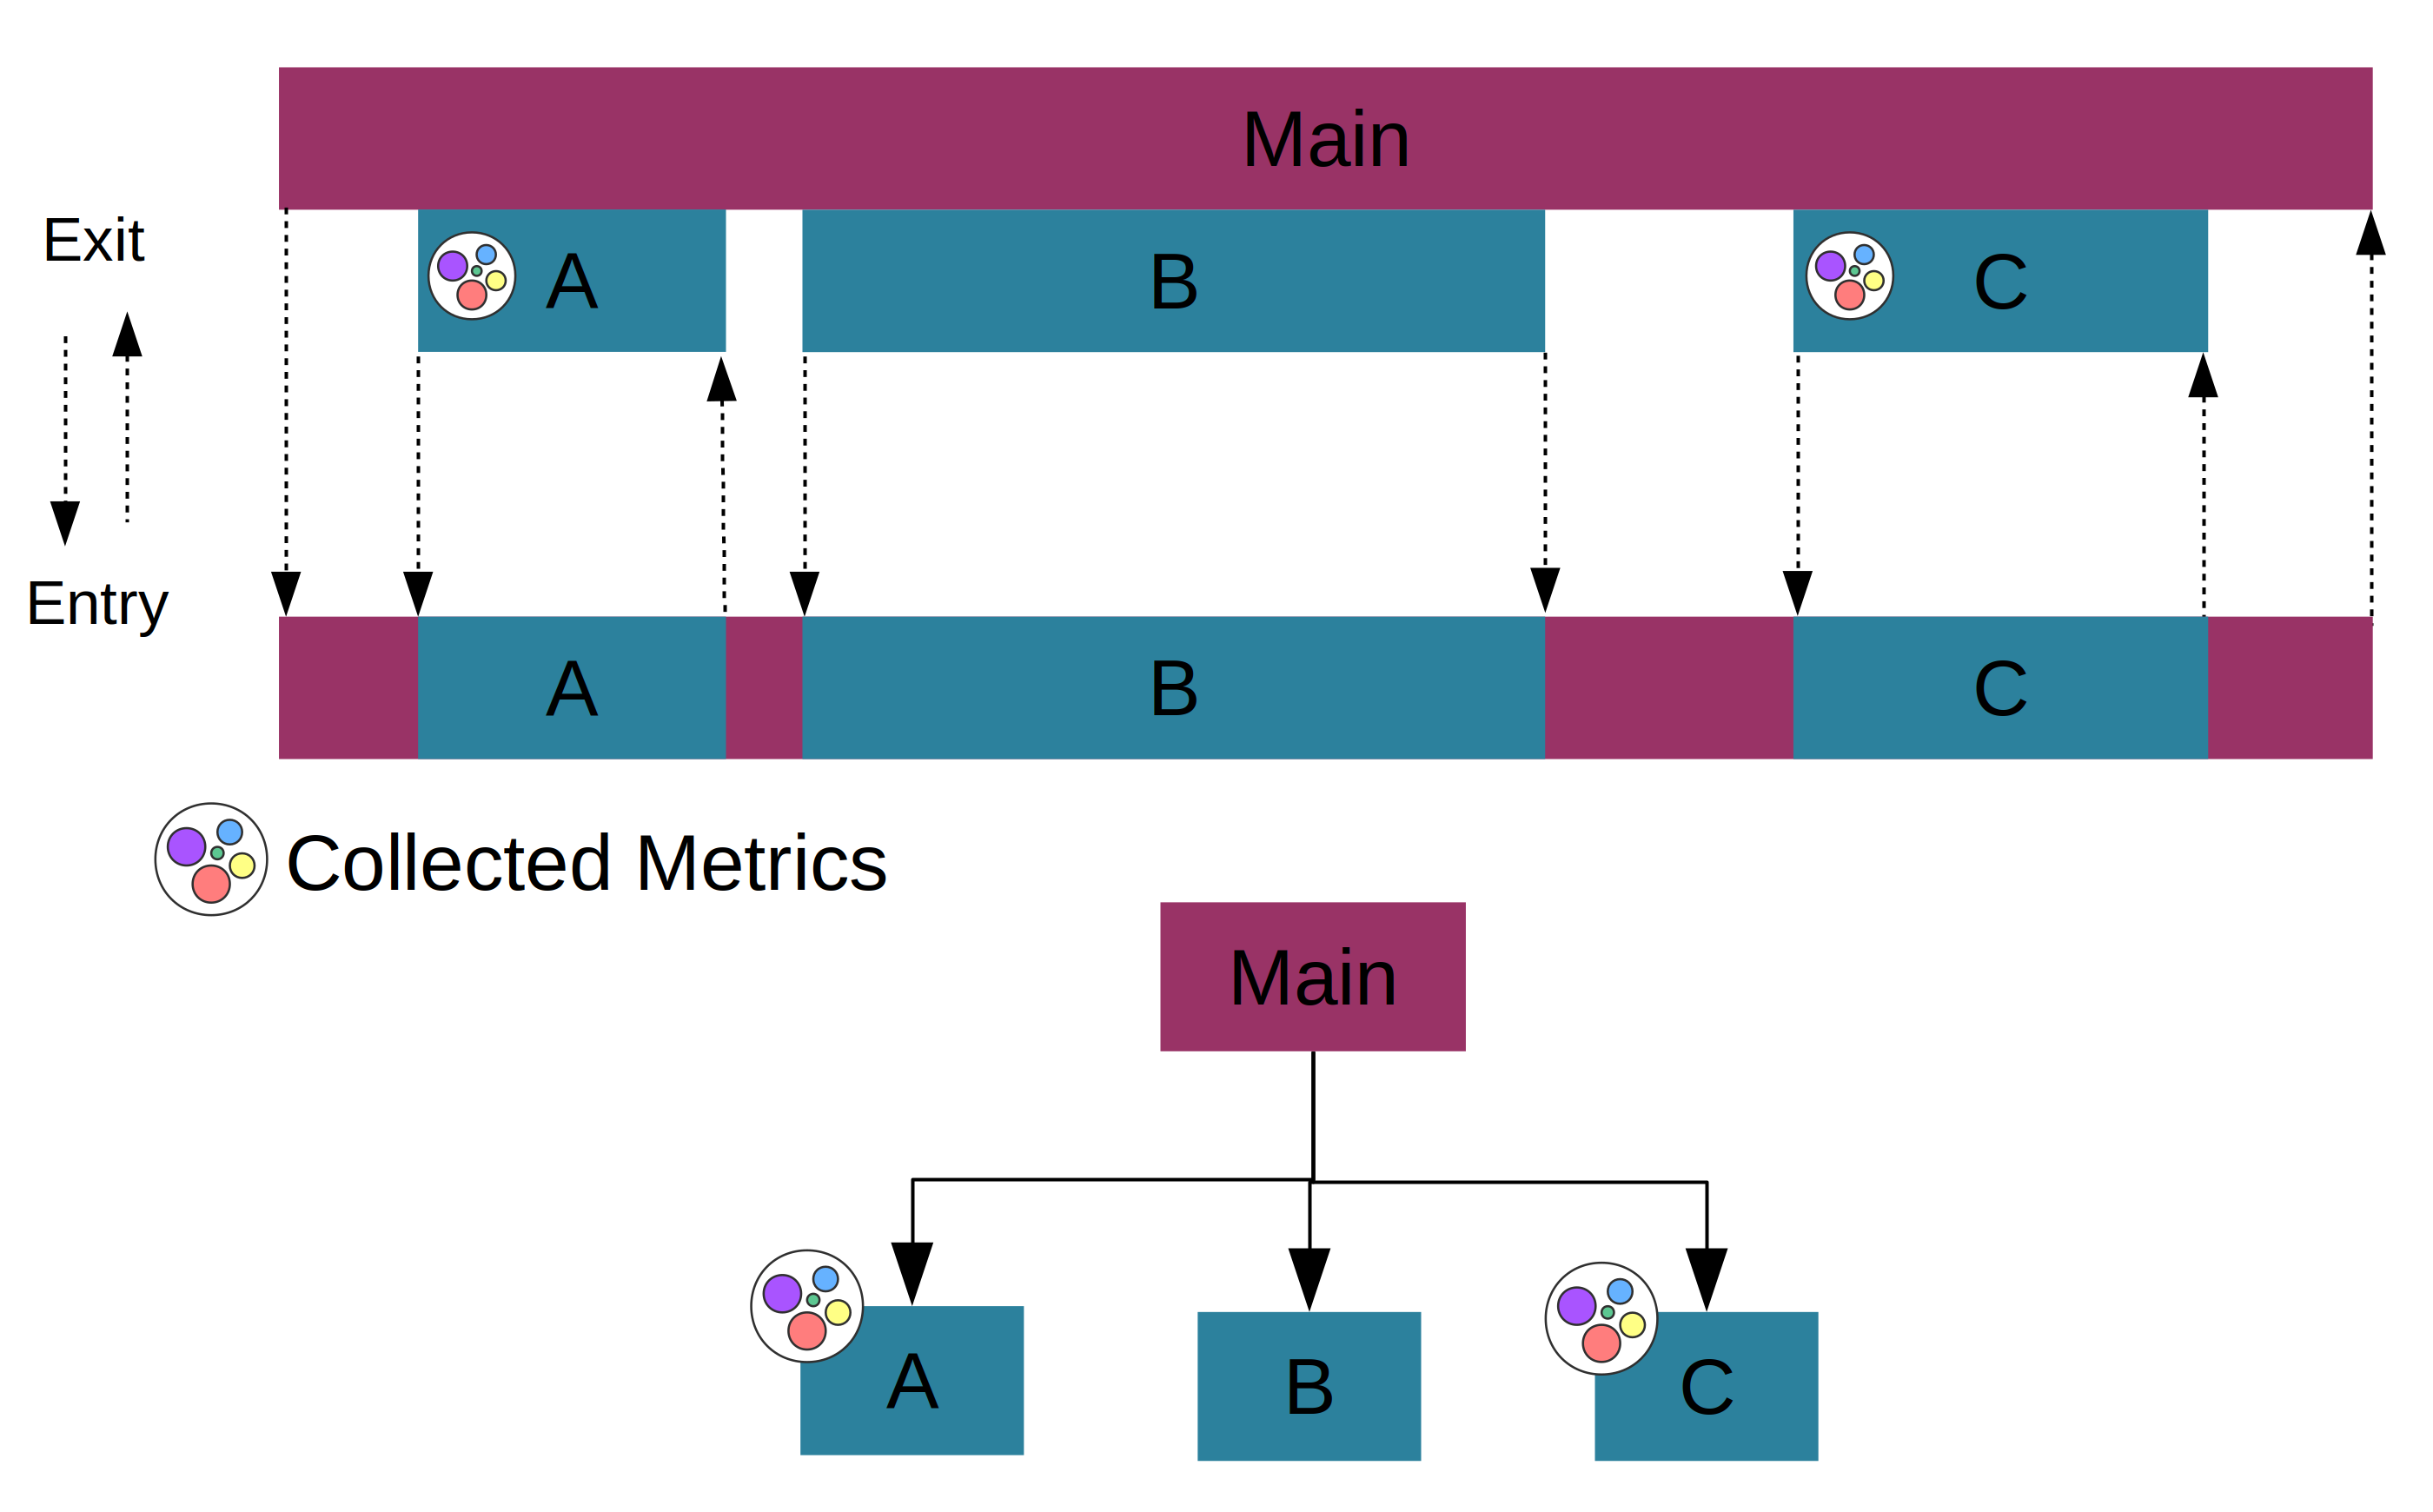
\includegraphics[width=0.50\textwidth]{figures/ecct.png}
        \caption{Enhanced Calling Context}
        \label{fig:ecct_build}
    \end{figure}
    
    After the construction of the tree the clustering mechanisms, described below, can be applied.\\
  
\subsection{Clustering}
\label{sec:clustering}
On this part we outline the clustering techniques used for the metrics grouping, the heuristic to do an automated classification mechanisms and finally the association rule used to find the metric which impacted on the performance of the executions.\\

% \textbf{Clustering techniques}
% \textit{ Supervised and non-supervised machine learn methods}\\
%     Supervised learning is the machine learning task of inferring a function from labeled training data. The training data consist of a set of training examples. In supervised learning, each example is a pair consisting of an input object (typically a vector) and a desired output value (also called the supervisory signal). A supervised learning algorithm analyzes the training data and produces an inferred function, which can be used for mapping new examples. 
    
%     Unsupervised machine learning is the machine learning task of inferring a function to describe hidden structure from "unlabeled" data (a classification or categorization is not included in the observations). Since the examples given to the learner are unlabeled, there is no objective evaluation of the accuracy of the structure that is output by the relevant algorithm—which is one way of distinguishing unsupervised learning from supervised learning and reinforcement learning.
    
\textit{Support Vector Machines}\\
In machine learning, support vector machines are supervised learning models with associated learning algorithms that analyze data used for classification and regression analysis. Given a set of training examples, each marked as belonging to one or the other of two categories, an SVM training algorithm builds a model that assigns new examples to one category or the other, making it a non-probabilistic binary linear classifier. 
Besides teaching the model, the restriction is another drawback of using SVMs. The major drawback of this model is the division in two groups, so relevant information could be lost and no further comparison technique could be applied later.

    
% \textit{Mean Swift}\\
%     MeanShift clustering aims to discover blobs in a smooth density of samples. It is a centroid based algorithm, which works by updating candidates for centroids to be the mean of the points within a given region. These candidates are then filtered in a post-processing stage to eliminate near-duplicates to form the final set of centroids.
%     Given a candidate centroid x i for iteration t, the candidate is updated according to the following equation:
    
%     %x_i^{t+1} = x_i^t + m(x_i^t)
    
%     Where N(xi) is the neighborhood of samples within a given distance around xi and m is the mean shift vector that is computed for each centroid that points towards a region of the maximum increase in the density of points. This is computed using the following equation, effectively updating a centroid to be the mean of the samples within its neighborhood:
%     %m(x_i) = \frac{\sum_{x_j \in N(x_i)}K(x_j - x_i)x_j}{\sum_{x_j \in N(x_i)}K(x_j - x_i)}
    
%     The algorithm automatically sets the number of clusters, instead of relying on a parameter bandwidth, which dictates the size of the region to search through. This parameter can be set manually, but can be estimated using the provided estimate bandwidth function, which is called if the bandwidth is not set.
%     The algorithm is not highly scalable, as it requires multiple nearest neighbor searches during the execution of the algorithm. The algorithm is guaranteed to converge, however the algorithm will stop iterating when the change in centroids is small \cite{mean_swift}.

\textit{Percentage classification}\\
The percentage classification was done by comparing the metrics and separate them by a percentage threshold, which is the mean of the group. The percentage classification is interesting considering sometimes that the distribution is not so spaced to create clusters. The naive classification will draw a group even when they are too close and would be in just one group for other clustering techniques.
    
\textit{K-means}\\
K-means is a simple unsupervised machine learning algorithm that groups a dataset into a user-specified number (k) of clusters. The algorithm is somewhat naive it clusters the data into k clusters, even if k is not the right number of clusters to use. Therefore, when using k-means clustering, users need some way to determine whether they are using the right number of clusters.
Since, the number of groups must be known before applying the k-means, another technique needs to be applied in order to find the appropriate number of groups (k). 
    
    
\textit{Comparing Models}\\
Comparing the three techniques described above, the conclusions were. First, the SVM model was able to delimit the difference between the slow executions and fast executions. However, the delimitation is in just two groups. \\
The second mechanism, Percentage classification, is a unsupervised mechanism and leads to segregation of data even if they are homogeneously distributed among the dataset. \\
Finally the k-means algorithm is efficient but requires the number of groups to be used in the classification process. Comparing the models we developed the technique to use an heuristic classification to make the clustering process automatic.
    
    
\textit{Auto Clustering}\\
Considering the models shown above, we chose to develop a non-supervised method, called auto clustering. The possibility to use an automated approach is more interesting for us in comparison with a non-automated methods, mainly because we aim not to use the data to train the model. Therefore we implemented a version of comparative k-means using the SSE (sum of square errors) variability information, plus an heuristic evaluation. This technique can be used for an arbitrary dimension of since the amount of difference, SSE (sum of squared error), can be calculated on those cases \cite{multi_dimentionals_sse}.
    
\subsection{\textbf{Automatic Clustering through heuristic Evaluation}}

    \textit{Elbow method}\\
    One method to quantitatively measure the number of clusters is the elbow method. This method compares the sum of squared errors (SSE) considering several numbers of groups from the classification used. 
    The elbow method gives the possibility to use the SSE to find the elbow value, which can be defined as a value which the SSE changes its behaviour abruptly. In our cases, the elbow value is when the SSE stop decreasing substantially.
    
    However, the elbow method does not guarantee a perfect match in cases which the data is well distributed. Instead, the analysis of the SSE can give a smooth curve and the best value for number of groups is not precisely defined. In cases like this, we developed another clustering based on the mean distance of the data.
    %try a different method for determining the optimal k, such as computing silhouette scores, or we might reevaluate whether clustering is the right thing to do on our data.
    
    \textit{Heuristic Evaluation}\\
    To compare the SSE values, we needed also to do an heuristic function which compares the different values of the SSE to compute the Elbow. 
    Therefore, we use this approach to compare several runs of classifications and extract the one with less squared errors. The used heuristic is to take as optimal group the biggest gap on an array of SSE values. 
    
    The Figure \ref{fig:sse}, shows an illustration of the SSE and the elbow value. The elbow value is the number that marks the change on the path of the function, in the example is number of groups 2.
    
    \begin{figure}[h]
      \centering
        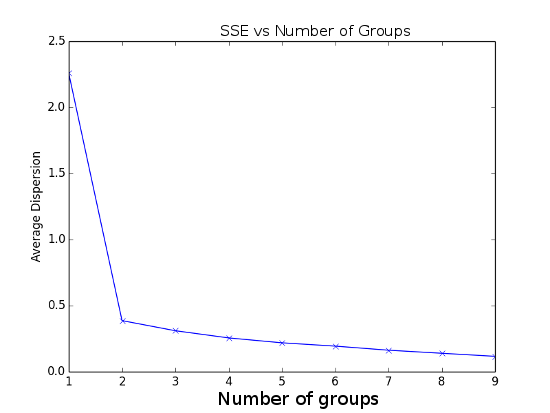
\includegraphics[width=0.50\textwidth]{figures/SSE.png}
        \caption{Elbow method: SSE Comparison}
        \label{fig:sse}
    \end{figure}


\subsection{\textbf{Association among the Groups}}
\label{sec:association}
The clustering of metrics is just a part of the approach, since a rule of groups need to be applied to find the specific cause for the discrepancy on the executions. To solve this problem and find the cause of the difference, after the grouping mechanism we applied a set association rule. Therefore, using a set exclusion, we can find the metric that is responsible for the elapsed time.
The association rule is illustrated on the Figure \ref{fig:association}, which describes a metric X and the elapsed time comparison. The grouping on the Metric x divides the data in two groups and those groups are the intrinsic related to the elapsed time group. \\
The association rule can be applied in an arbitrary classification algorithm with several different dimensions, so the association can be defined as a heuristic to find root cause problems using grouping or clustering algorithms.

A matrix of groups correlation can be done to better understand the relation among the groups.


    % \begin{figure}[h]
    %   \centering
    %     \includegraphics[width=0.50\textwidth]{figures/association.png}
    %     \caption{Association of groups through Apriori algorithm}
    %     \label{fig:association}
    % \end{figure}
    
\begin{table}[h]
\centering
\begin{tabular}{cccc}
                      & A                         & B                        & C     \\ \hline
                      &                           &                          &       \\ 
A                     & X                         & 75\%                     & 100\% \\ \hline
                      &                           &                          &       \\ 
B                     & 75\%                      & X                        & 65\%  \\ \hline
                      &                           &                          &       \\
\multicolumn{1}{l}{C} & \multicolumn{1}{l}{100\%} & \multicolumn{1}{l}{65\%} & X     \\ \hline
\end{tabular}
\vspace{10pt}
\caption{Association of groups through Apriori algorithm}
\label{fig:association}
\end{table}

\subsection{\textbf{Accuracy of the model}}
The association will give the group of metrics that are related with slow and fast runs, however, there is the possibility of false positives and false negatives. The accuracy of the model is related with the size of the groups given, i.e. the all slow executions will be in one group, however the related metric, which explains the reason, is bigger than the associated group.  In summary, if the groups overlap, main metric and slow executions, no false positives of negatives were found, even though the overlap does not mean is responsible for the performance problem, it is only an indication factor. In this matter, statistics is an indicator of underlying causes, which requires some complementary analysis to be confirmed.
    
    
\section{Solution Implementation}
\label{sec:implementaion}
\begin{figure*}[t!]
  \centering
    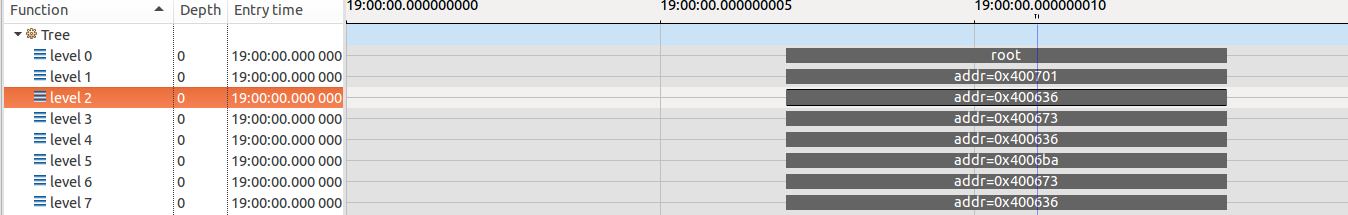
\includegraphics[width=1.0\columnwidth]{figures/cct_view.png}
    \caption{CCT View in TraceCompass }
    \label{fig:cct_view}
    \vspace{-10pt}
\end{figure*}

We describe on this section the implementation of the Calling Context Tree in TraceCompass, the Flame Graph comparison, and the Auto cluster mechanism.

The CCT View is an analysis developed in TraceCompass framework \cite{tracecompass}, which specifically aims to study the CCT and its variations. The module with Auto clustering was included on it. The view displays the calling functions in a graphic view that helps the developer/tester to improve their codes and to compare the traces using the approach described on this work.\\

\textbf{\textit{Tree Construction}}\\
The CCT View builds the tree from the tracing as explained in the section Tree Construction. In summary the tracing is read in order and event entry-exit pairs are grouped in nodes, sub-nodes are defined by pairs of entry-exit inside the above node. The data found, i.e the performance metrics, of the nodes is summarized for the respective node. The tree is build to summarized the redundant nodes, thus, avoiding the build of a Dynamic Call Tree. Figure \ref{fig:cct_view}, shows this feature in the CCT View.\\

\textbf{\textit{Differential Flame Graph}}\\
The CCT View implements a Differential Flame Graph view to compare executions and groups of executions. Usually the Differential Flame Graph compares two executions, but on our implementation it is possible to compare groups of executions. In our implementation the flame graphs are composed of three colors: green (to represent equals amount of time), red (slower executions) and gray (faster executions). 

Figure \ref{fig:flame}, shows a diagram of the RGG Differential Flame Graph, the green color shows the functions which are faster in the main execution, the grey part means they are equal and the red part means that this function is slower with the comparative one. The name, RGG flamegraph brings allusion of this concept in contrast with Brendan Gregg's Red/Blue Flame Graph. 
 
 \begin{figure}[h]
  \centering
    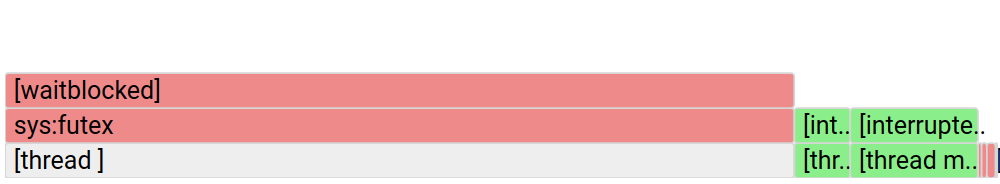
\includegraphics[width=1.0\textwidth]{figures/framegraph.png}
  \caption{RGG Differential Flame Graph Diagram}
  \label{fig:flame}
\end{figure}

\textbf{\textit{Auto cluster}}\\
The Auto cluster feature was implemented on CCTView to help developers execute similar performance cause analysis on tracing. The heuristic evaluation (elbow method) and the clustering techniques (k-means and percentage clustering) were implemented separately, therefore the developer can choose the most suitable one.\\
    
\textbf{\textit{Correlation feature}}\\
Another feature of the CCT View is the possibility to find the correlation matrix of the metrics. 
As the dictum states, \textit{correlation does not imply causation}, which means that correlation by itself cannot be used to infer a causal relationship between the studied variables.
        
    

\label{sec:methodology}
% BENCHMARKS    --------------------------------------------
\section{Benchmarks}
    Considering the several aspects of software performance, here are highlighted some micro-benchmarks which can impact on the performance of the software and could change the performance of software throughout the releases.
    
    \textit{inline}\\
    The inline functions are a C++ enhancement feature to increase the execution time of a program. Functions can be compiled as inline automatically, or can be declared by the programmer as inline functions. The compiler replaces the definition of inline functions at compile time instead of referring function definition at runtime.
    
    However, those functions do not always improve the performance and can deteriorate the performance \cite{inline_site}. To evaluate this claim, we tested this feature with several possibilities: strings, integers, structs, vectors, and classes. Using the inline made the performance better for all of them, except for std::string operations. 
    
    The reason for this difference possibly is related with the dynamic allocation time of strings in C++ as explored by \cite{optc++}. We did several tests with different data structures and objects, and strings seems the more effected by this effect.
    
    After investigation, we came to the conclusion that the root cause of this performance degradation is the influence of cache misses in the operations with string inside inline functions.
    
    Comparing the performance of inline functions and regular functions, the results of the benchmarks are shown in the Figures \ref{fig:notinline} and \ref{fig:inline}. For thousand runs, the average, the mean and the median were high in comparison to use the not inline implementation.
    
    \textit{template functions} \\
     Template functions can decrease the performance of a software.
     According to Jacob B. Matthews, from the university of Chicago, \cite{chicago}, the use of templates decrease efficiency of the C++ compiler's.
     
     
    \textit{virtual functions} \\
     The use of virtual functions has a cost for the dispatching. The work of \cite{dispatch} shows the overhead related with dispatching on C++ codes.
     
    \begin{figure}[h]
      \centering
        % 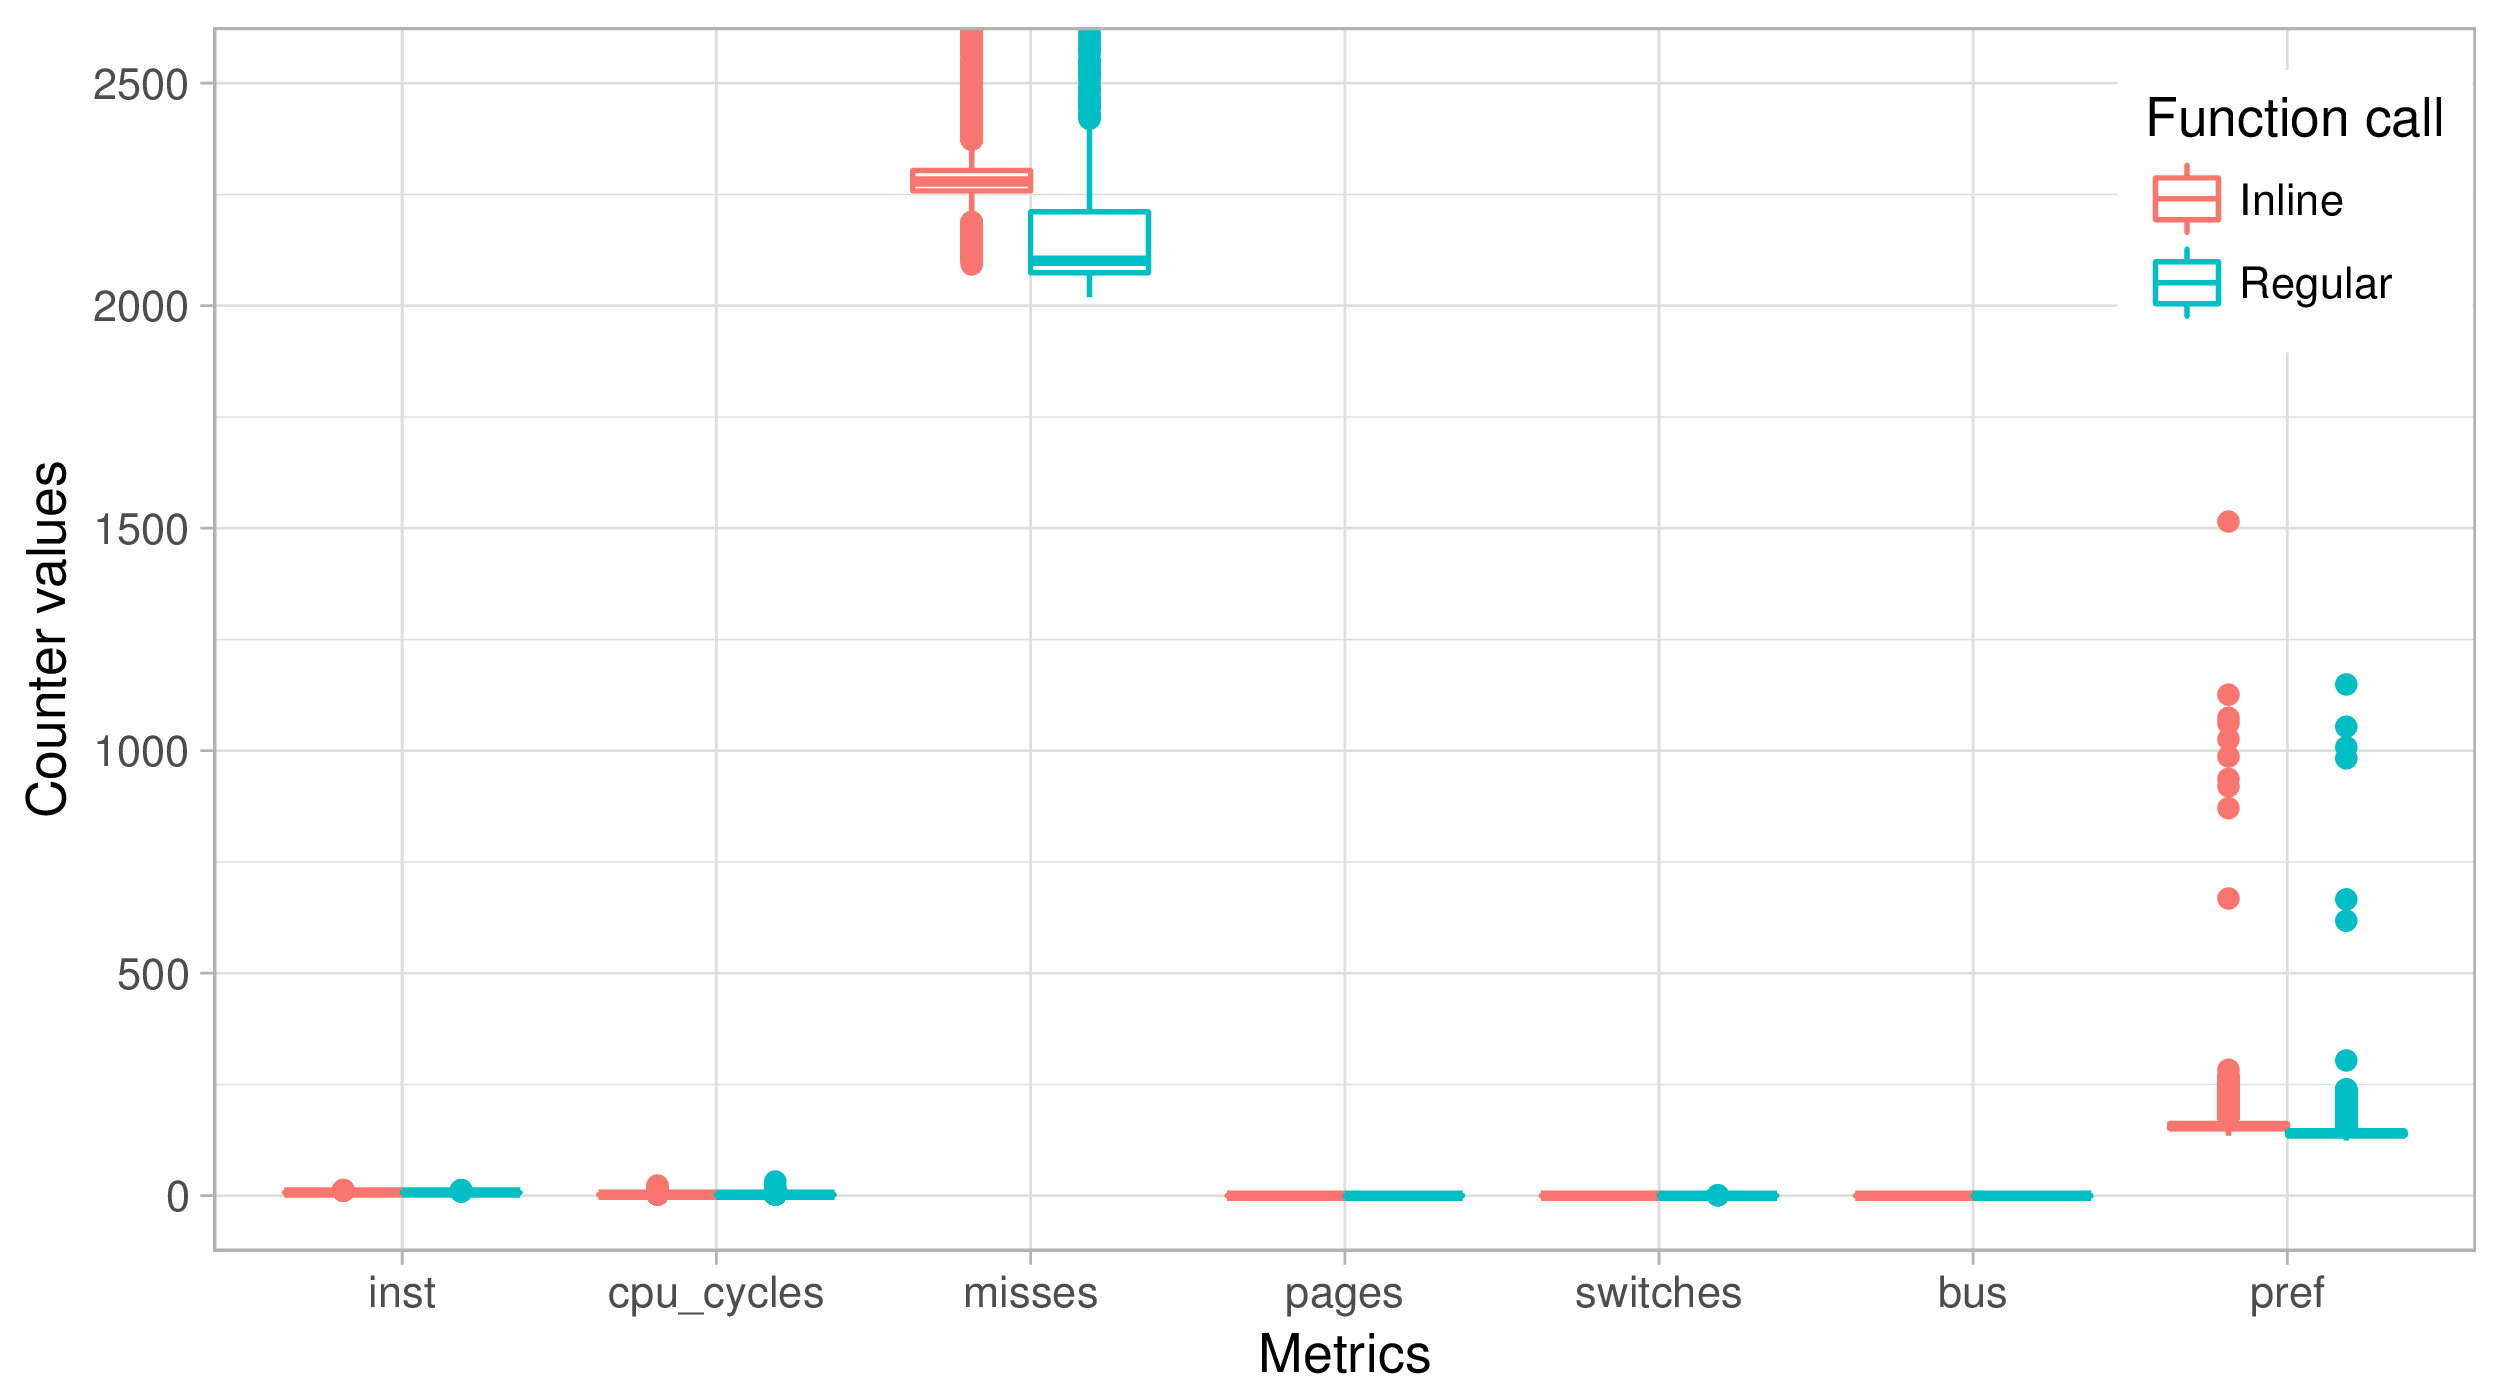
\includegraphics[width=0.47\textwidth]{figures/boxplots-inline-vs-regular.png}
        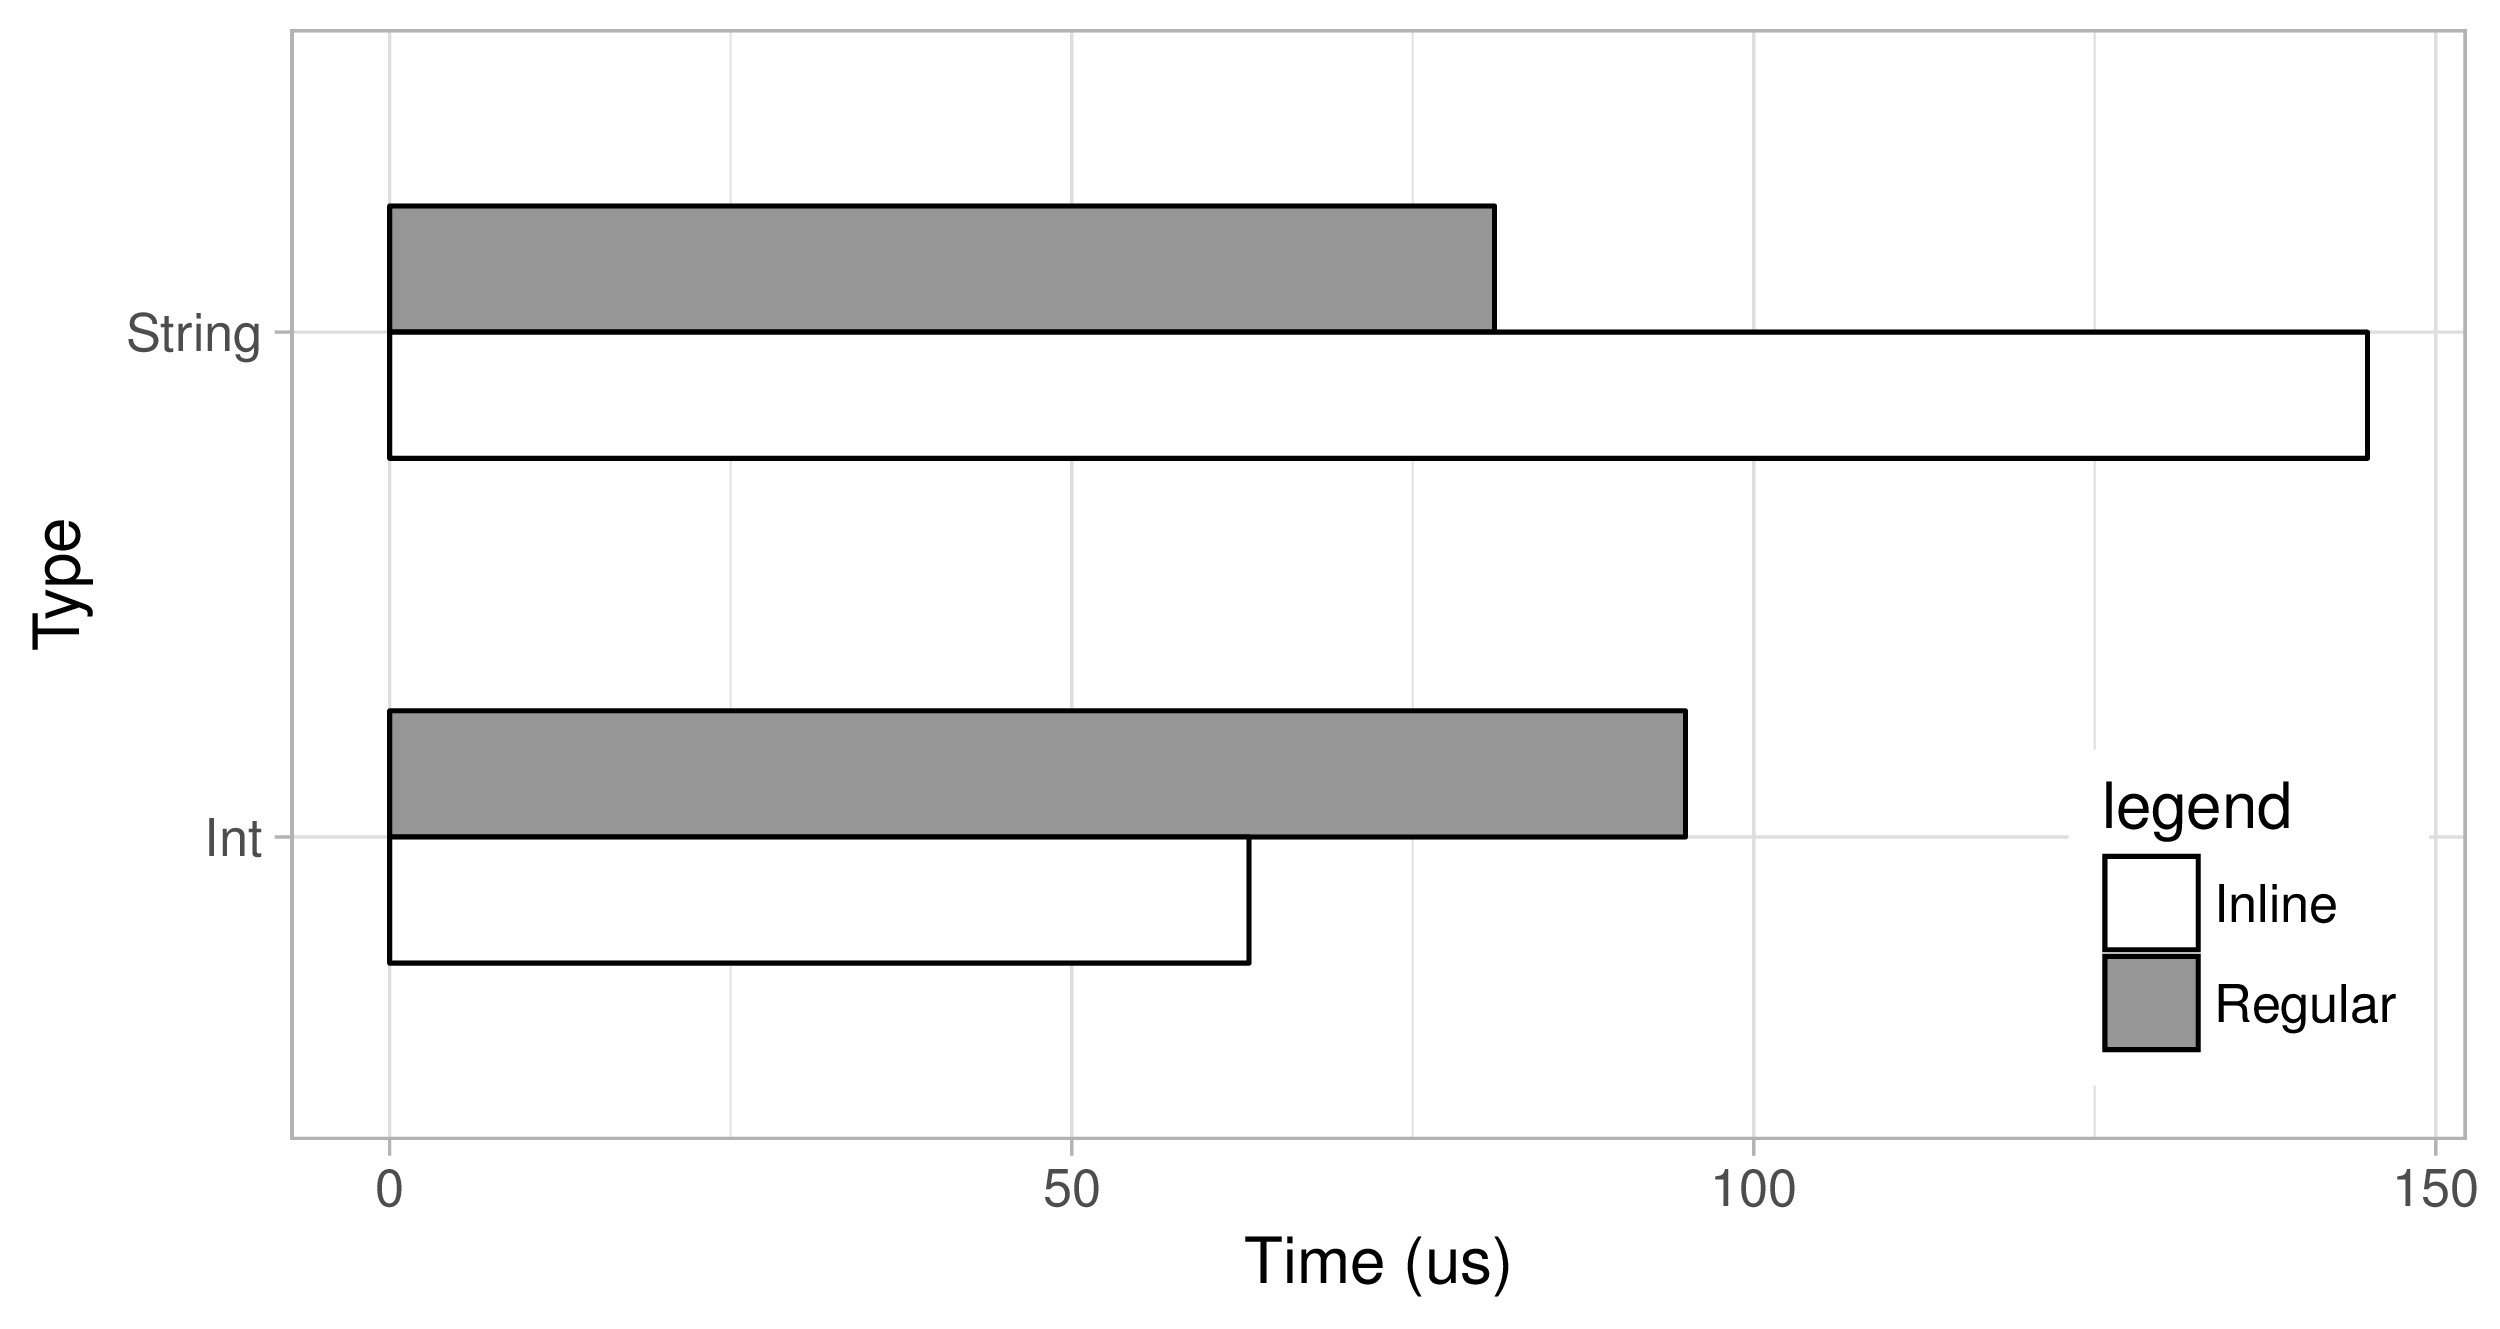
\includegraphics[width=0.6\textwidth]{figures/bar-inline-vs-regular.png}
        \caption{Counter Metrics for Inline and Regular function calls}
        \label{fig:notinline}
    \end{figure}
    
    \begin{figure}[h]
      \centering
        % 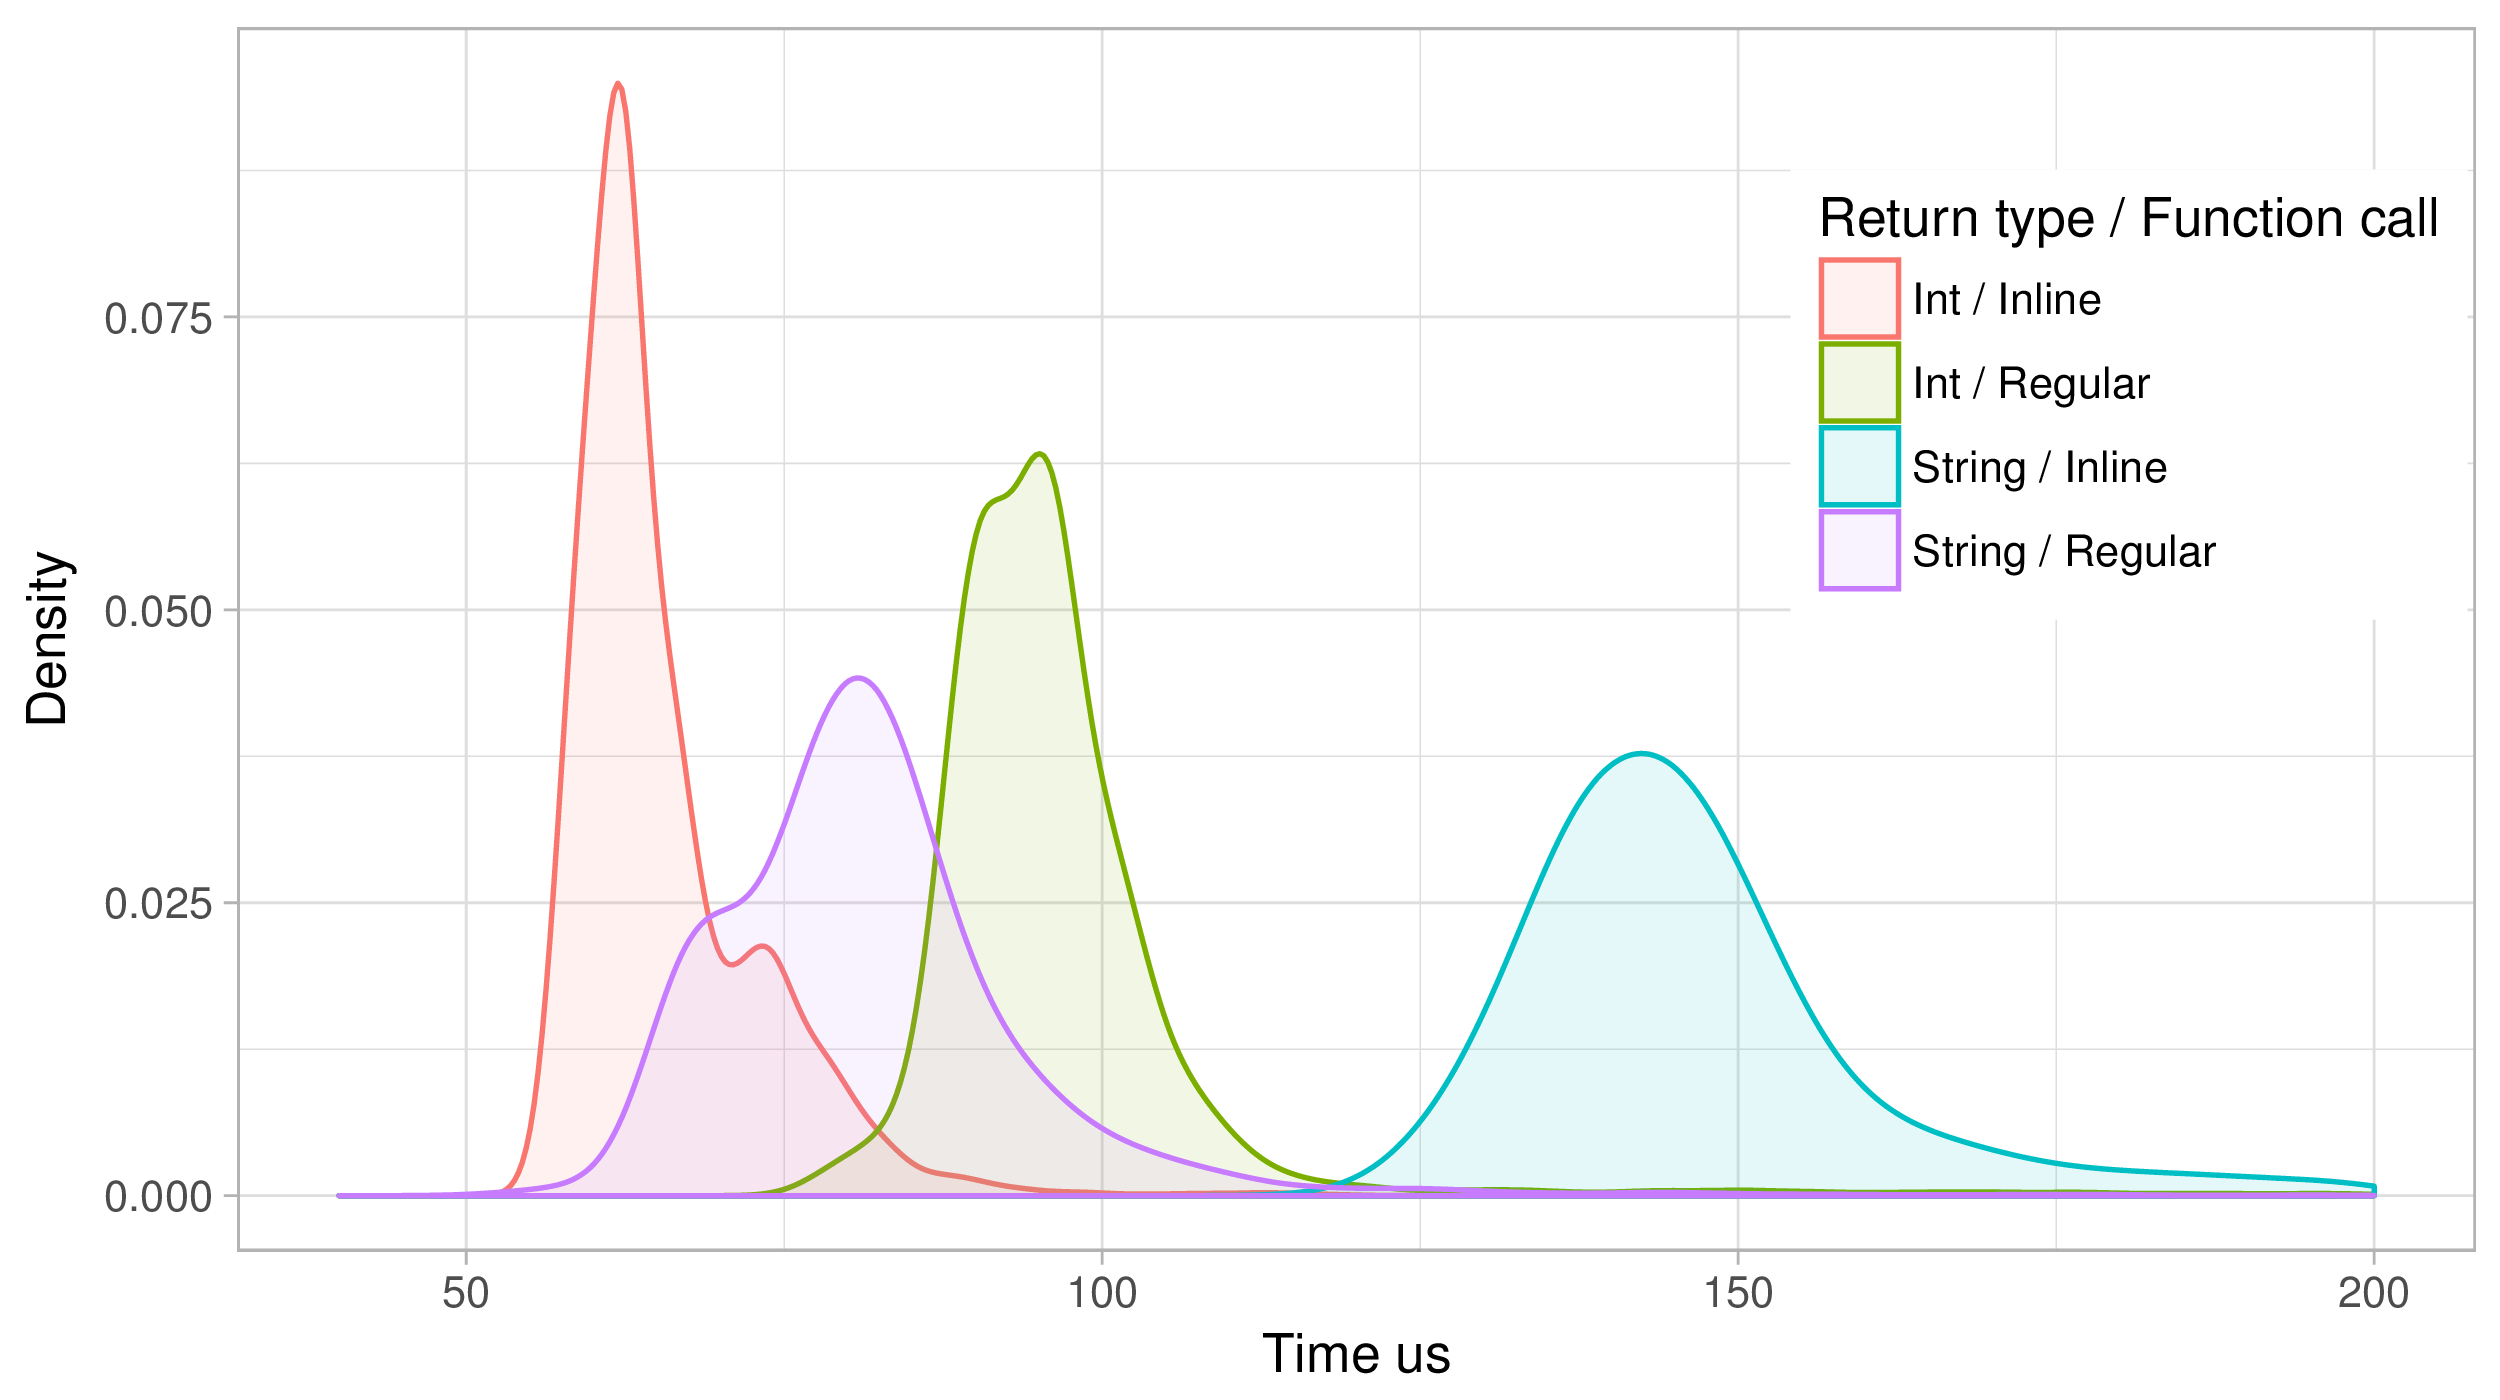
\includegraphics[width=0.47\textwidth]{figures/density-inline-vs-regular.png}
        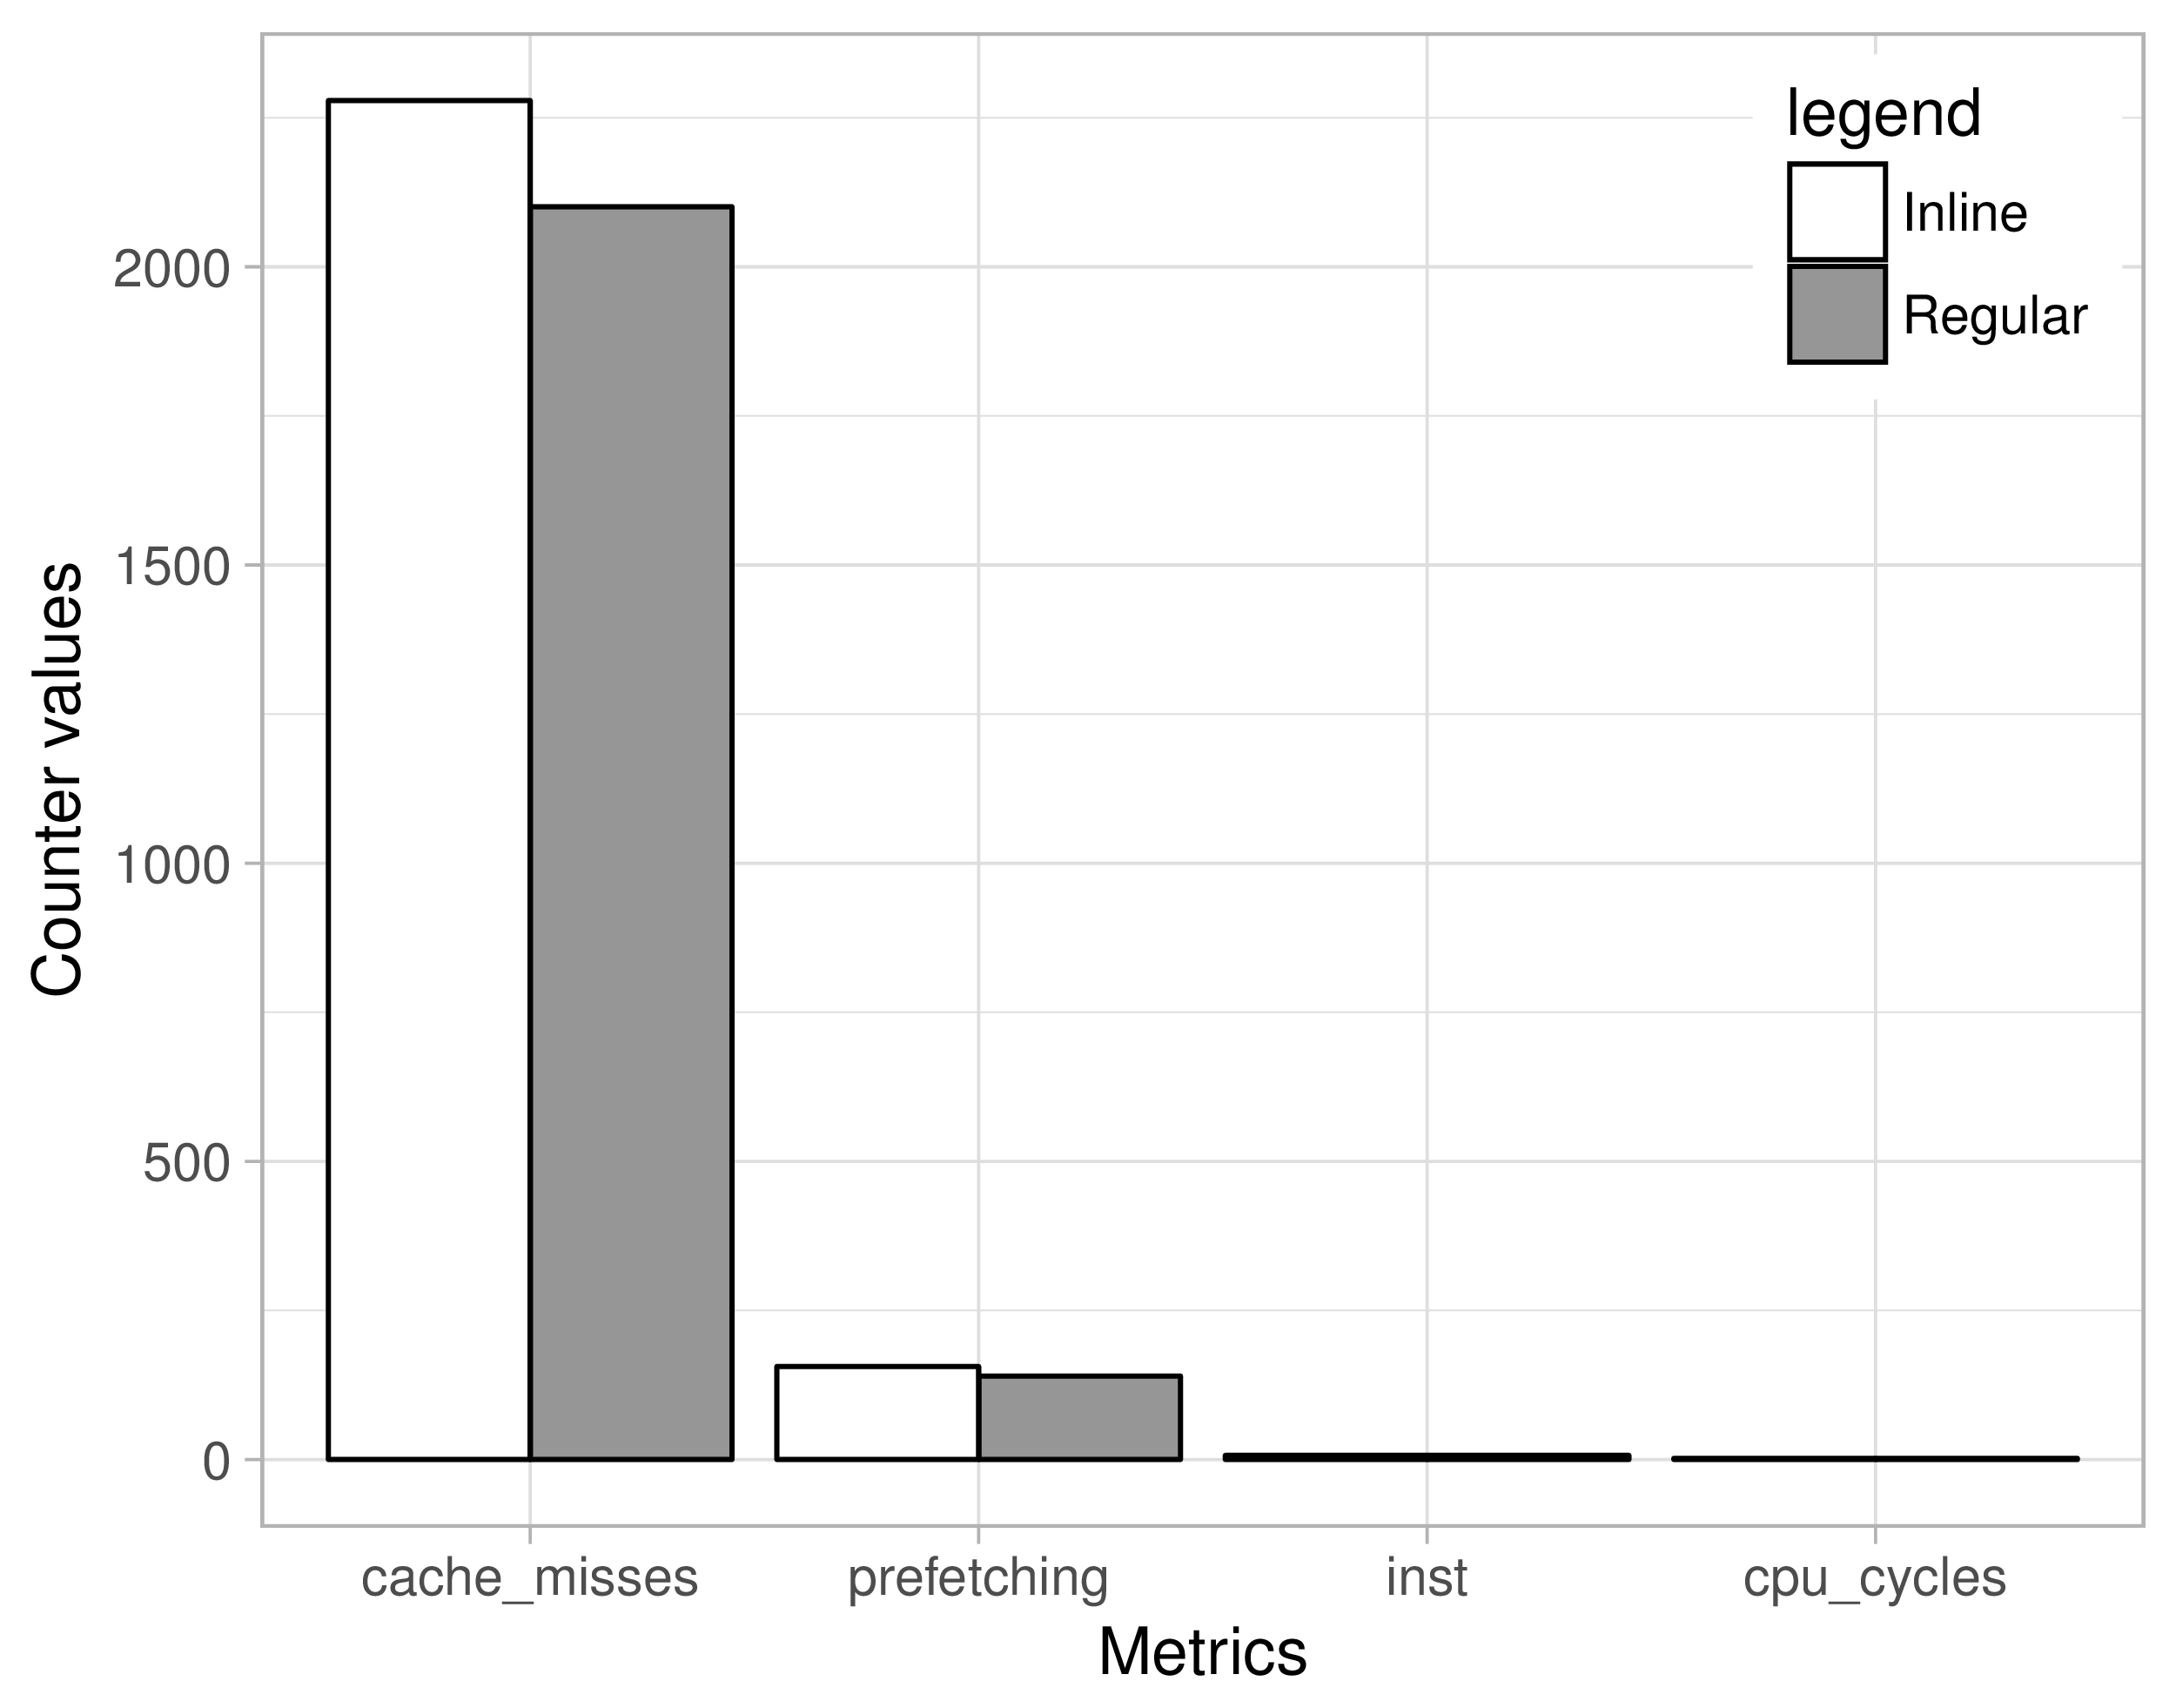
\includegraphics[width=0.57\textwidth]{figures/barplots-inline-vs-regular-counters.png}
        \caption{Distribution of Inline vs Regular functions using String and Integer as return types}
        \label{fig:inline}
    \end{figure}
    
    
    \section{Illustrative Example}
    
\textbf{Open Close}
    To illustrate the approach used, we developed a small code which does several times the process of opening a file subsequently. The code was instrumented with -finstrument functions and this gave the possibility to run the code using Lttng-UST.
    When execute this code several times, some executions have a different behaviour, which we call outliers.
    Using our approach, first we record the executing metrics of the program, then the automated cluster technique is applied, finally we compare the groups: slow executions and fast executions. We deduced that the problem was related with the wait-cpu time metric on the slow executions.
    
    The figure \ref{fig:group} demonstrates the grouping mechanism, which segregated the executions in two groups, the association rule related all the slow executions with wait-cpu group 2 and the fast executions with wait-cpu group 1. The association showed that the wait-cpu was the cause for this difference of the groups.
    
     \begin{figure}[h]
      \centering
        % 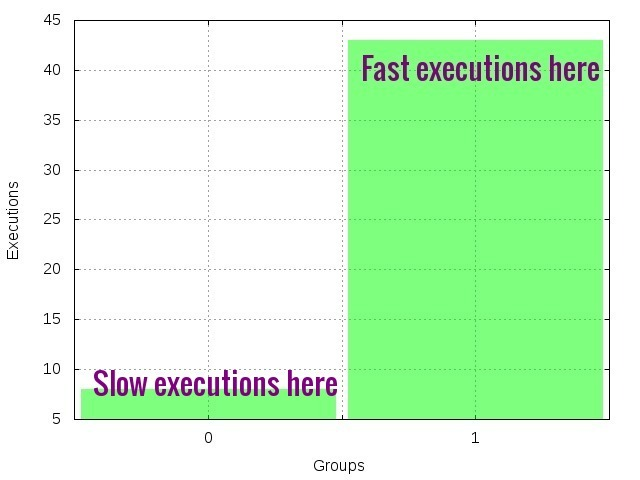
\includegraphics[width=0.50\textwidth]{figures/grouping.jpg}
        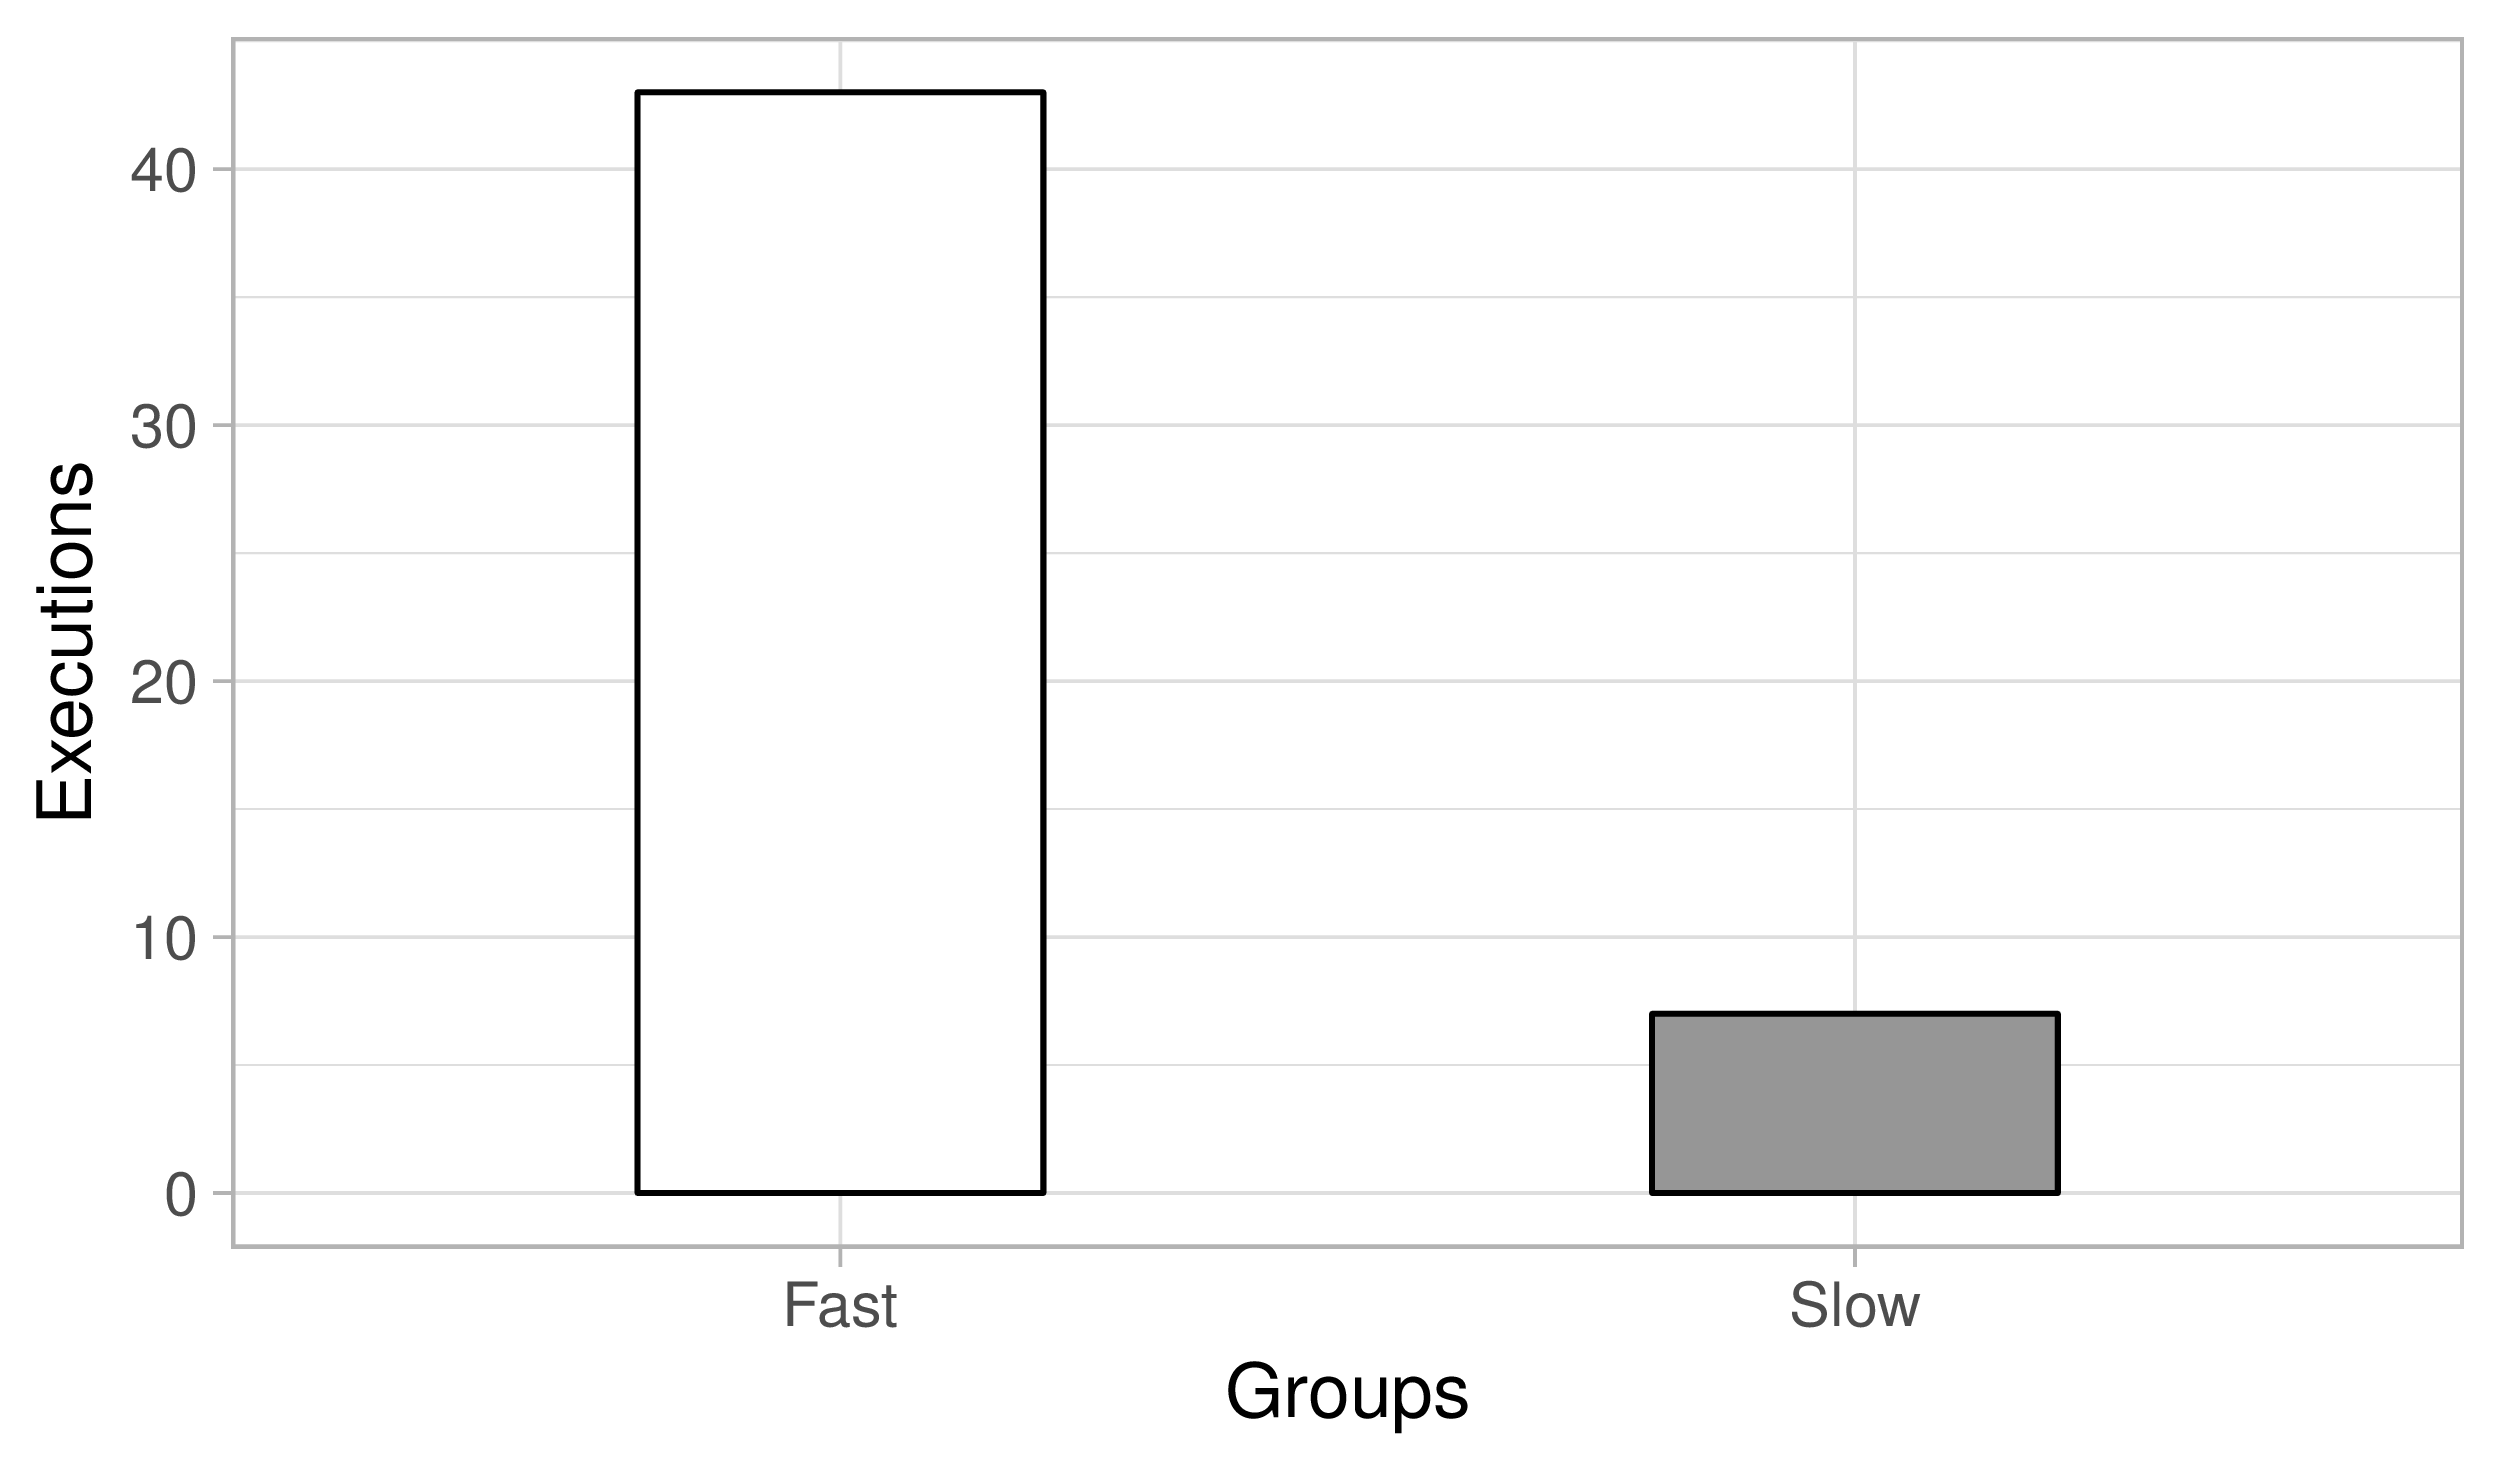
\includegraphics[width=0.65\textwidth]{figures/open-program-groups.png}
        \caption{Comparing executions of Open program}
        \label{fig:group}
    \end{figure}

    
    
\textbf{Executions}
    All experiments were done in a computer with a quad-core Intel® CoreTM i7-3770 CPU running at 3.4 GHz, 16 GB of DDR3 memory and a 7200 RPM hard drive. The Linux kernel version was 3.13.0-49 while the LTTng version was 2.6.0.
% \subsection{\textbf{Scheduler Interference}}
  
% \subsubsection{Summary}
%     A process is executed with lower priority than another, which is triggered on regular intervals. The scheduler plays its role to change the process order at regular times on Linux systems.
    
% \subsubsection{Approach}
%     Our approach was to run the process several times to trigger the conflict with a task with higher priority. While running it, we recorded the tracing data. Then, we executed our clustering analysis and classified the data in several groups. Were able to find that on the fast runs the execution took: x milliseconds. However, on not normal executions - slow executions.
    
% \subsubsection{Results}
%      Were able to find that on the fast runs the execution took: x milliseconds. However, on not normal executions - slow executions. The automated comparison showed that the main difference was on the x function.

    

% \subsection{\textbf{Regression Comparison}}
    
% \subsubsection{Summary}
%     A new feature was added on the new software version and the performance regressions tests are showing a slightly performance difference with a feature, which uses inline functions.
    
% \subsubsection{Approach}
%     Our approach was to run the software several times with the function using and not using inline. The tool was applied from the tracing data. The benchmarks used showed that strings operations with inline can have a difference performance.
    
% \subsubsection{Results}
%     The functions using inline were a little worst in terms of performance to non inline versions. The classification result showed that inline were related with a larger number of cache misses indeed.

%     Figure \ref{fig:case1}, shows the grouping results relating the cache misses with the slow executions groups.
    
%     \begin{figure}[h]
%           \centering
%             \includegraphics{figures/inline.png}
%             \caption{Case study Regression - showing differences on the runs using inline functions and not inline}
%             \label{fig:case1}
%     \end{figure}


\section{Case Studies}
\label{sec:usecases}
We used our approach on the following use cases:

\subsection{Regression Comparison}
    
\subsubsection{Summary}
    A software company is releasing its new version of software with several new features. The performance regressions tests did not find problems and the unitary tests were accepted. Some weeks after the release, the users started to complain about performance issues in one of the features.
    
\subsubsection{Approach}
    Our approach was to run the software several times on the previous and in the current version of the software. Then classified the data using our approach in slow and fast executions. 
    
    \begin{figure}[h]
      \centering
        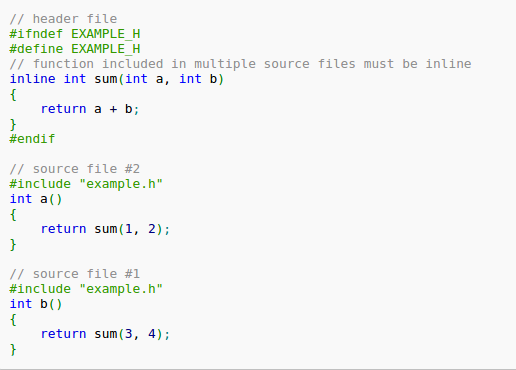
\includegraphics[width=0.50\textwidth]{figures/inline_example.png}
        \caption{Example of Code for inline}
        \label{fig:caseOpt}
    \end{figure}

\subsubsection{Results}
    Were able to find that in-line function addition on the feature increased the number of cache misses and therefore increased the elapsed time of this application. On the source code the in-line functions could be seen as difference although the developers thought that this would improve and not decrease the performance.
    
    Using a comparative approach of the groups we could see the difference of the metrics withing them. Comparing the groups of in-line functions and the groups without inline, we verified that the inline groups comparatively to their respective groups of non-inline, had a significant amount of cache misses. Concluding that cache misses was the essence of the differences.
    
    Table \ref{tab:table}, shows the grouping results relating the cache misses with the slow executions groups comparatively. 
    
\begin{table}[]
\centering
\caption{Table Performance}
\label{tab:table}
\begin{tabular}{ll}
\hline
\multicolumn{2}{c}{Executions}                        \\ \hline
Fast group                & Slow group                \\ \hline
mean of 2500 cache misses & mean of 6500 cache misses
\end{tabular}
\end{table}

\subsection{Page Faults Interference}
    \subsubsection{Summary}
    A program executes several times the process of writing on the buffer, the process reveals a problem after several sub-sequential executions.
    
\subsubsection{Approach}
    Our approach was to run the process several times to trigger this problem. The mechanism classified the executions according to the execution time and also for the metrics.
    
\subsubsection{Results}
     The tree generated had branches with fast and slow executions, 
     The classification was done within the branches of the tree and we were able to find that for all the fast executions (group fast on elapsed time), the group of page-faults were in the first group. On the slow executions, the page-faults were classified on another group. So, the tool revealed the association, and we can conclude that the program triggers more page faults specifically after several executions.\\
     The company was not able to track this problem before because of the prefetching algorithms influence of the executions. This technique is used on the microprocessor architecture to speedup the instructions. The Figure \ref{fig:case1}, is a CCTView result that shows this  difference on the runs on several runs.
    
    \begin{figure}[h]
          \centering
            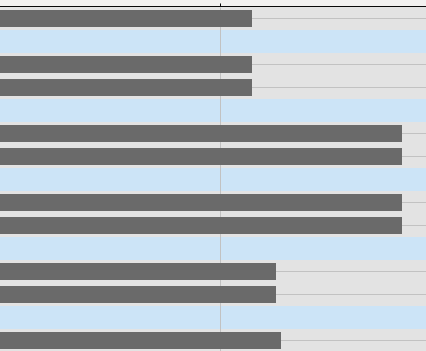
\includegraphics[width=0.50\textwidth]{figures/showing_diff.png}
            \caption{Case study Regression - Tree details showing significantly differences on the runs, where the faster are smaller and the slower are bigger in the images}
            \label{fig:case1}
    \end{figure}
    % Figure \ref{fig:case3}, shows the grouping results relating the page-faults grouping with the slow executions groups.

    
\subsection{Cache Optimization in Server Application}
    
\subsubsection{Summary}
    A server application using a very known content-management framework caches requested data to improve the time access of its content. However, around 1000 requests, the cache is flushed and needs to be redone. So specifically on this request the server will spend more time than on the previous requests.
    
\subsubsection{Approach}
    Our approach was to execute several times a request for a server. While running it, we recorded the tracing data. Then, we executed our clustering analysis and classified the data in several groups.
    
\subsubsection{Results}
    The tree generated by the tool was able to display that on the fast group no time was spent on cache or compile time. However, on slow executions, there was a considerable time spent on compilation time and cache time.
        
    \begin{figure}[h]
      \centering
        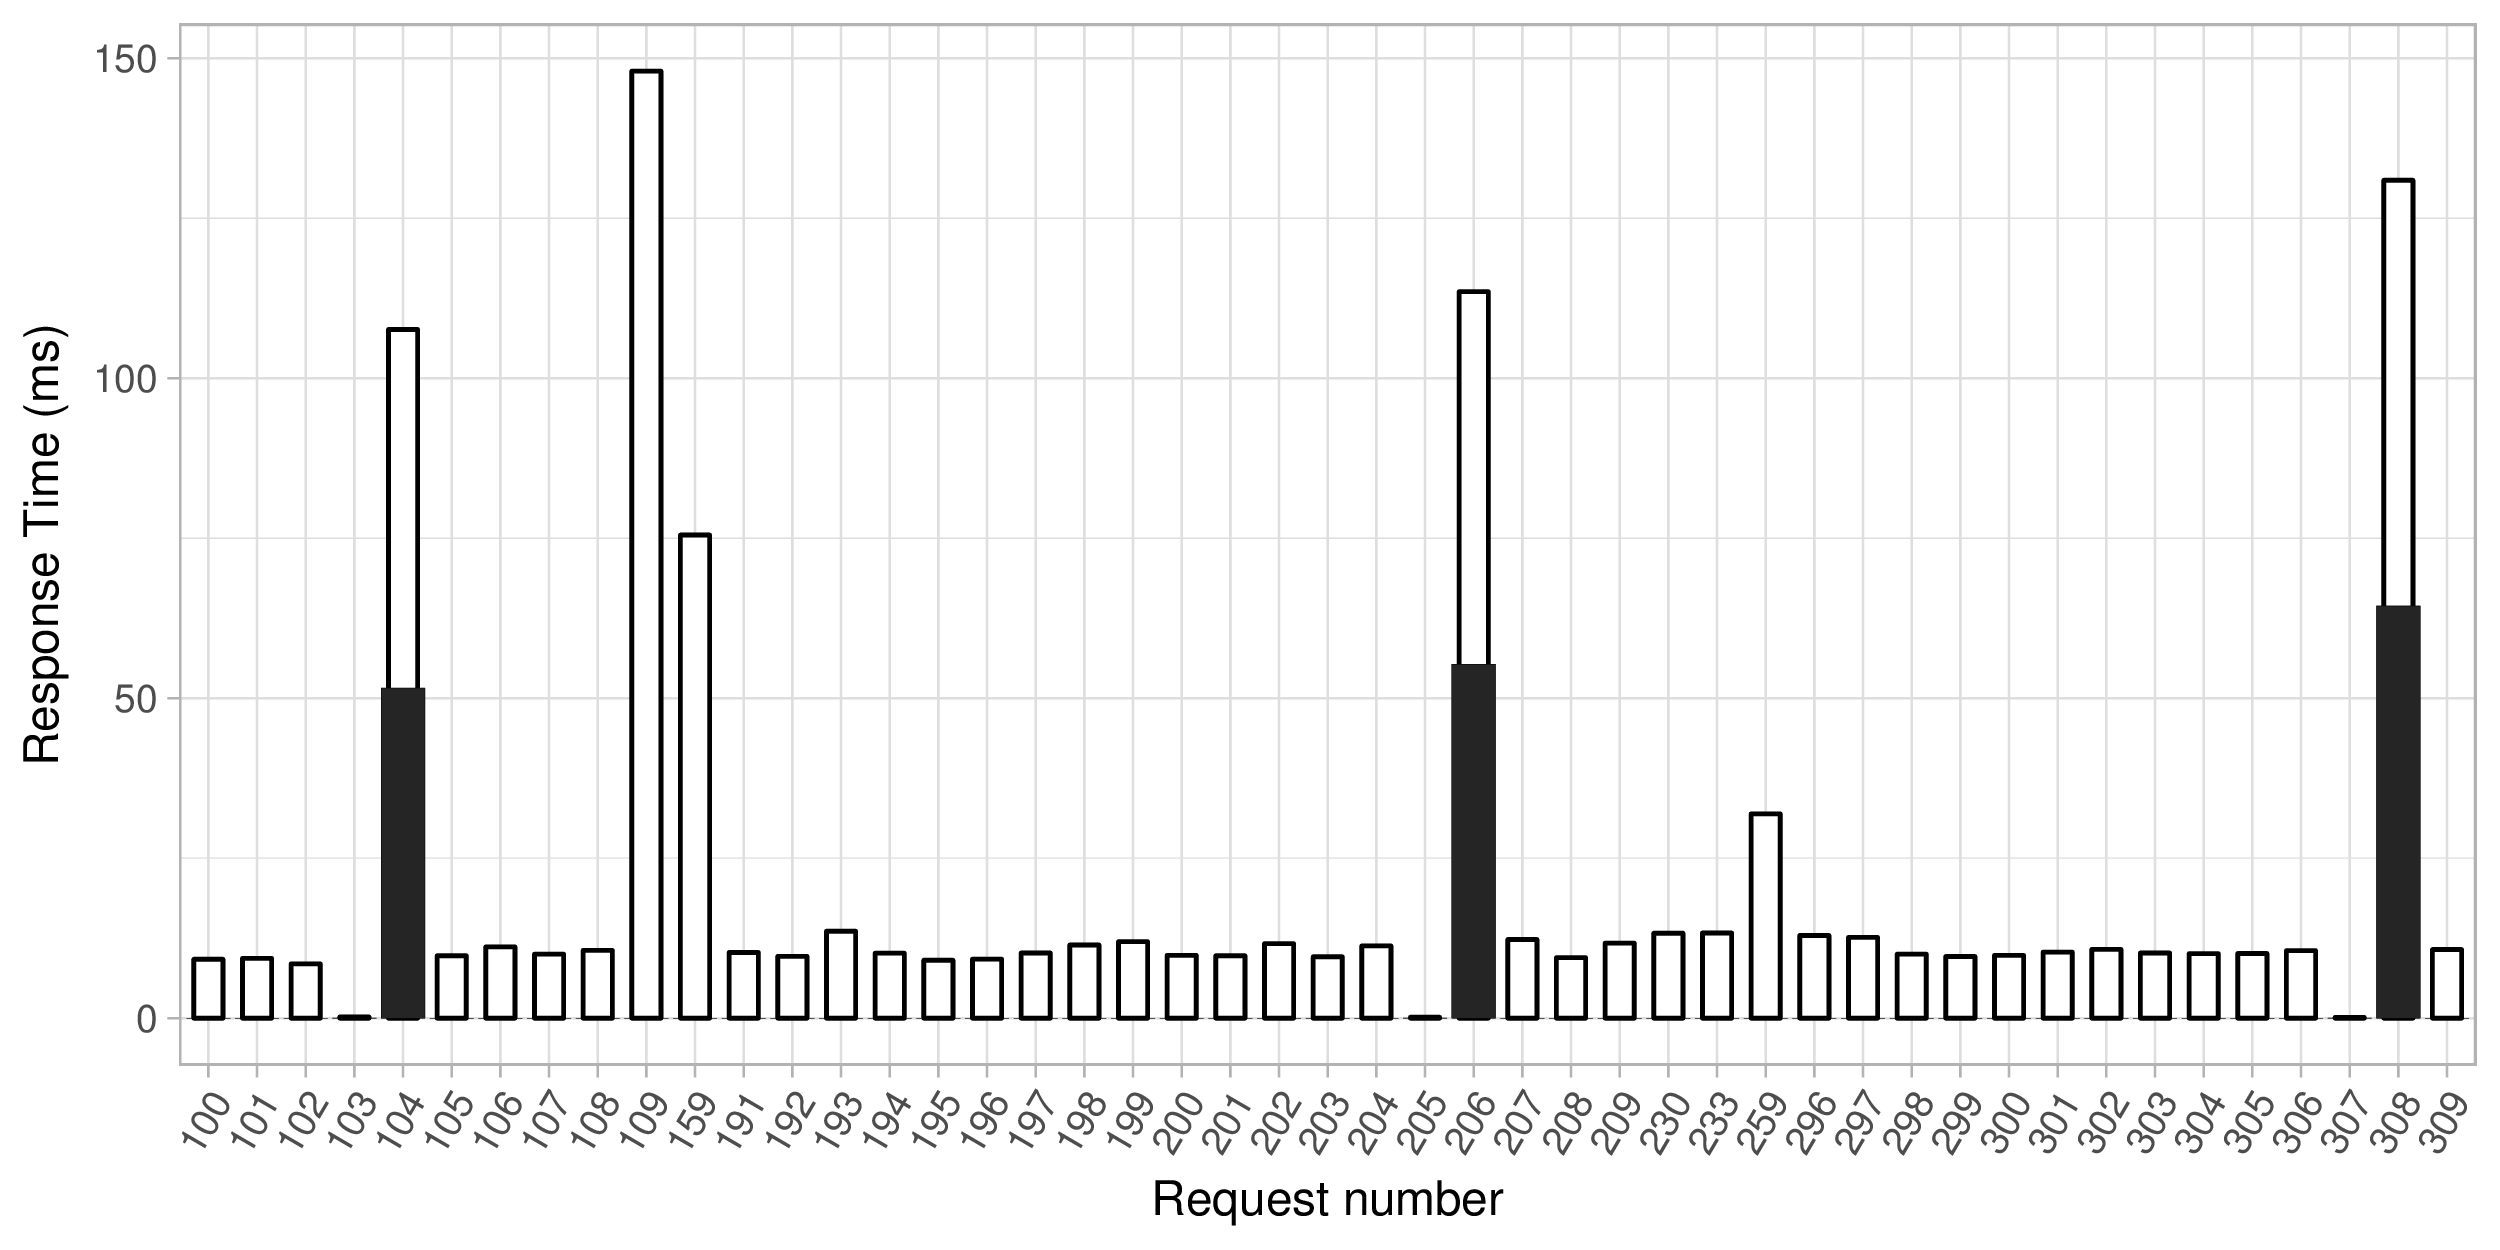
\includegraphics[width=0.50\textwidth]{figures/server-time-series-bar.png}
        \caption{Overhead introduced by I/O for caching on each 100 of requests, The white bat represent the request response time and the dark bar represent the PHP compilation time}
        \label{fig:server-time-series}
    \end{figure}
    % Figure \ref{fig:case4}, shows the grouping results relating the page-faults grouping with the slow executions groups.
    
    
\subsection{Json Cpp}
\subsubsection{Summary}
    JSON is a lightweight data-interchange format. It can represent numbers, strings, ordered sequences of values, and collections of name/value pairs.

    JsonCpp is a C++ library that allows manipulating JSON values, including serialization and deserialization to and from strings. It can also preserve existing comment in unserialization/serialization steps, making it a convenient format to store user input files.
    
    Executing several times the reading from json file, some of the executions have a different time to read those files.    
    
\subsubsection{Approach}
    Our approach was to run the software several times and run the clustering technique then compared the metrics between the groups.
    The auto-grouping technique showed more than 10 groups to be compared, but only a few were taken in consideration.
    
\subsubsection{Results}
    The solution showed differences on the branches of the tree and was able to display the relation with scheduler switches and the performance of this task, this would impact directly on a real task. All the tasks that took more time were related to task scheduling and switches.
    
    
\subsection{OpenCV}
Open Source Computer Vision Library (OpenCV) is an open source computer vision and machine learning software library. This library is used in different problems in computer vision as tracking image. In this section, we will benchmark Optical Flow and HoughLines algorithms, which they are the most evolving features in the recent years.

\subsubsection{Optical Flow} 
The Optical Flow, implemented as Lucas-Kanade algorithm, is an example of method in OpenCV and aims to correlates the apparent motion of objects between two consecutive frames. From some examples of the book \cite{opencv2_book}, this method can be tested with two images and show differences on them. Regressions can be caused by a series of changes on the code. Doing the tests we found a relevant regression on the function Optical Flow.

\textbf{Approach}: Our approach was to run the software several times recording performance metrics using Linux Perf Events. The elapsed time to track the performance is also used in the classification. The runs were related with several versions of OpenCV until find the regression between the versions 2.3.0 and 2.3.1, where the latest version was around 5 times slower than others.

\textbf{Results}: The results correlate the longer duration with more instructions so we could see on the code that a conditional statement was different from version to another, which makes the slower to execute more instructions. This regression was originally reported on \cite{regression_opencv}.
The total number of commits on those two versions were about 250 commits, using this technique, it was able to reduce the difference for about few lines of code and unit tests can be made to trigger specifically this cause after knowing that it is a cache misses problem.

Figure \ref{fig:OpenCV}, shows the result of the optical flow in from two images.
    
\begin{figure}[h]
      \centering
        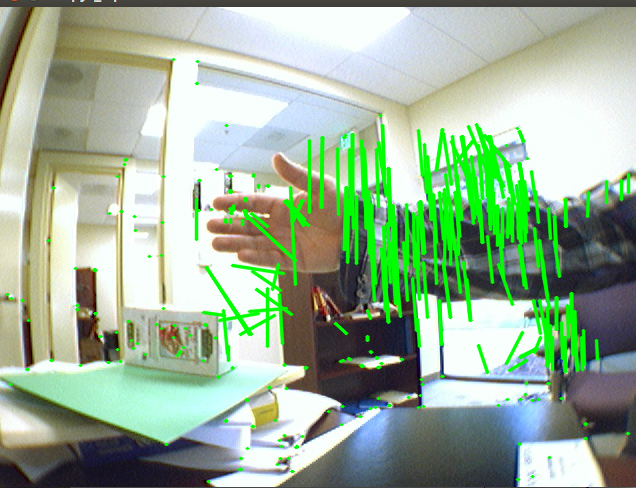
\includegraphics[width=0.50\textwidth]{figures/flow.png}
        \caption{Optical Flow Example}
        \label{fig:OpenCV}
\end{figure}

\subsubsection{HoughLines} 
HoughLines is a line detection mechanism implemented in OpenCV, to find edges in images. This can be used to find edges in roads and it is implemented algorithm is called Canny86. While comparing different versions of opencv, we found that version 3.1 takes more time than version 3.0. in a case of Software Regression, \cite{timeTests}. The source code difference can be found here \cite{opencv_source_diff}.

\textbf{Approach}: Our approach was to run the software several times recording performance metrics using Linux Perf Events in a large file. The elapsed time to track the performance is also used in the classification. The runs were related with several versions of OpenCV until find the regression between the versions 3.1 and 3.0, where the newer version was slower than the previous one.


\textbf{Results}: The results correlate the longer duration associated the longer runs with cache misses. By analyzing the code we were able to find a difference on the file hough.cpp, related with a difference size of the called array. This process reduced the 
    
    Figure \ref{fig:case2}, shows the grouping results relating the cache misses with the slow executions groups.
    
    \begin{figure}[h]
          \centering
            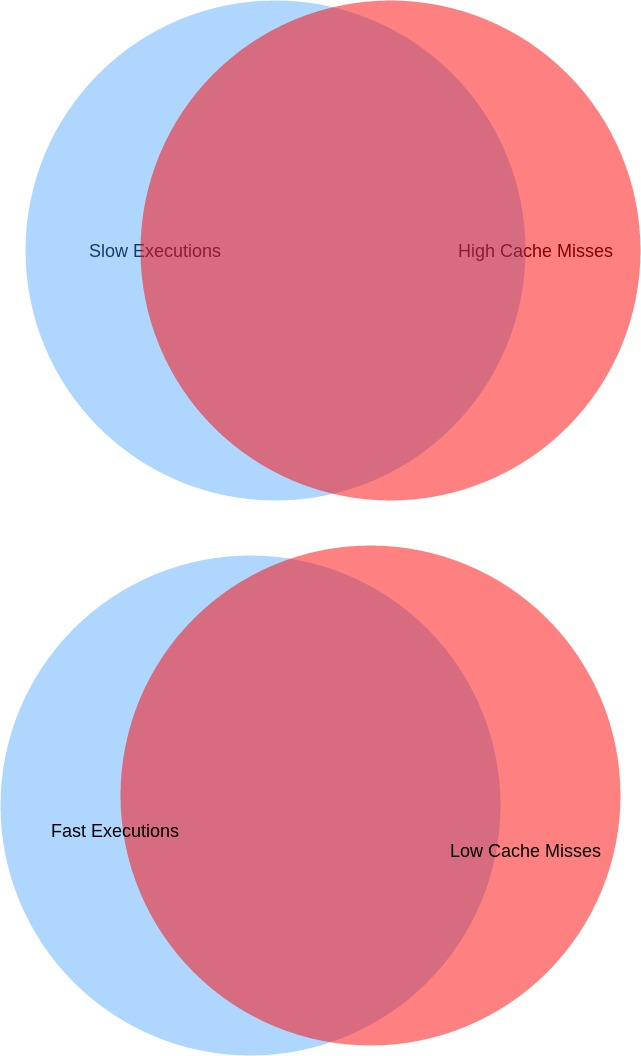
\includegraphics[width=0.350\textwidth]{figures/set_results_cache.jpg}
            \caption{Case study Regression - showing significantly differences in the groups of runs in terms of metrics.}
            \label{fig:case2}
    \end{figure}
    
\subsection{Regression Comparison II}
    
\subsubsection{Summary}
    A software company deployed several new packages in its software including a buffer implementation change. There was a performance impact on this change but it is not possible to track specifically which commit caused the impact. The company would need to run specific Linux commands to find the reason for this problem or reproduce several performance tests with each commit. This scenarios was taken from \cite{essentials} also related to Microsoft bug in \cite{microsoft_bug}.
    
\subsubsection{Approach}
    Our approach was instrument the code and to run the software several times on the previous and in the current version of the software. Then classify the data using our approach in slow and fast executions, although the auto-grouping gave more groups, i.e. reduction of ten to two groups of comparison.
  
\subsubsection{Results}
      The tree generated had branches with fast and slow executions aggregated together. The nodes recorded the several performance metrics including the instructions, cache misses and page-faults.
      We were able to find that page-faults extra addition addition on the feature decreased the performance.
      On the source code, the change on the buffer was an array that was implemented using a row major storage scheme and caused an addition of about 16.384 page faults.
      
      
% \subsubsection{Results}
%      The tree generated had branches with fast and slow executions, 
%      The classification was done within the branches of the tree Figure \ref{fig:case1}, we were able to find that in-line function addition on the feature increased the number of cache misses and therefore increased the elapsed time of this application. On the source code the in-line functions could be seen as difference although the developers thought that this would improve and not decrease the performance.

    The code in highlight shows the difference on the array coding that created the page-faults difference. This code was taken from \cite{essentials}.
    
    % \begin{figure}[h]
    %       \centering
    %         \includegraphics[width=0.2\textwidth]{figures/pf_use_case.png}
    %         \caption{Case study Regression Comparison II - code changes}
    %         \label{fig:caseX}
    % \end{figure}
    
The Figure \ref{fig:k-means} shows the use of k-means with 2 as k number of groups.

    \begin{figure}[h]
          \centering
            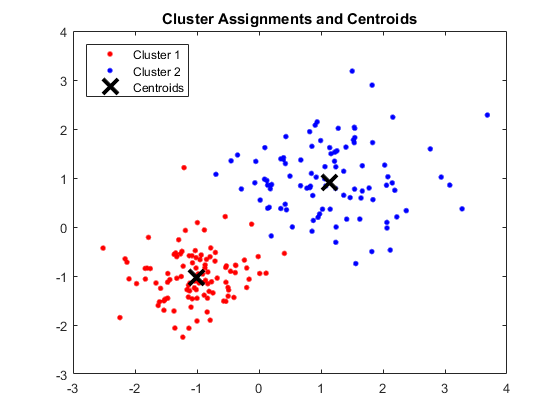
\includegraphics[width=0.50\textwidth]{figures/k-means.png}
            \caption{K-means result}
            \label{fig:k-means}
    \end{figure}
    
    
% \begin{lstlisting}
% #include <stdio.h>
% #define N 10
% /* Block
%  * comment */

% int function1()
% {
%     int i;
%     int i, j;
%     int[128][128];
% }
% \end{lstlisting}

\lstset{language=C++,
                basicstyle=\ttfamily,
                keywordstyle=\color{blue}\ttfamily,
                stringstyle=\color{red}\ttfamily,
                commentstyle=\color{green}\ttfamily,
                morecomment=[l][\color{magenta}]{\#}
}
\begin{lstlisting}

    //Considering 128 words/page\\
    
    int i, j;\\
    int[128][128]; \\
    // original version\\
    for(i = 0; i < 128; i++)\\
        for(j = 0; j < 128; j++)\\
            data[i][j] = 0;\\
    // new version\\
    for(j = 0; j < 128; j++)\\
        for(i = 0; i < 128; i++)\\
            data[i][j] = 0;\\

\end{lstlisting}
% \label{pseudo:page-faults}
% 
% \caption{Case  study   Regression  Comparison   II  -  codechanges}
 


\section{Discussion}
\label{sec:results}
% Present the results for your research questions. For each one, provide a short motivation (why is this question important to answer?), brief overview of analyses used (of those discussed in \autoref{sec:approach} and your actual results. For each individual result of a research question, put a first sentence in bold, then use the rest of the paragraph and possibly follow-up paragraphs to explain the result. Do this for each result of a question, and all questions.

This section presents a discussion related with the research questions presented on the introduction, as well as, the solution presented. The results of the use cases clarifies the research questions delimited on the introduction and conduct new insights on this performance part.

\begin{itemize}

\item RQ 1: How can we build an efficient and flexible model for performance comparison?\\
    Using the enhanced calling context tree it is possible to aggregate performance metrics and compare executions efficiently. The CCT can be built with or without source code modification. The possibility to build it without source code brings the opportunity to analyze the dynamic structure and an accurate behaviour can be used.\\
    
\item RQ 2: Is it possible to automate the performance analysis?\\
    Our work demonstrated the possibility to use non-supervised machine learning methods to compare and find performance problems, specifically using a comparative heuristic technique. The approach used is to use a comparative clustering mechanism, which can efficiently separate the data for a realistic comparison.\\
    
\item RQ 3: How accurate was the obtained results?\\
    The methodology used was able to find association between groups of metrics and consequently associate the cause of elapsed time variations. However this approach can have type I or type II errors - false positives and false negatives.
    
\end{itemize}

% The solution presented was able to automate the process of clustering by using a deterministic heuristic comparison.



\section{Threats to Validity}
\label{sec:validity}
This section discusses the threats to the validity of our study.\\
\textbf{Time analysis}
    Our approach is based on comparing several clusters to take the best according to the SSE, which requires a comparatively long period of time. Our study aims to use an automated non-supervised clustering method, thus the analysis time is a minor factor if it is less than human analysis. Although the analysis required just a few minutes between building the ECCT tree and the classifying the metrics. Another highlights is that the analysis is made offline, so the time will not influence on the performance of the software and does not require stopping the software development.
    
\textbf{Quantity of groups}
    Considering the automated heuristic used can give a high number of groups for evaluation. This process can increase the difficult for evaluation.

\section{Future Work}
\label{sec:fut}
As future work, we plan to expand our investigation by using non-linear models to track regression problems in different software versions\cite{deep}. This can be used as an automated test to find software regressions. An example of possible models are feed-forward network, ibidem, also called deep learning networks.
The models need to be able to characterize specifically non-linear dependencies and be able to be used without non label data.\\ 
% Considering those restrictions, an Autoencoder or a Restricted Boltzmann Machine are also candidates.\\ 
%This require modifications in the loss function.

Another possibility would be to apply other techniques such as Apriori algorithm, \cite{apriori}, which can determine association rules among the metrics recorded in the enhanced CCT, for each cluster. Finally, tracking performance issues before the release of new software is an interesting path to be followed. Thus, an automated mechanism to find them before the release of a new version of software is very promising. A possibility could be to develop a mechanism to be executed as a regression test suite, from the machine learning models described above, before the releasing.



\section{Conclusion}
\label{sec:conclusion}
% In conclusion, this research developed a solution that showed the possibility to use clustering mechanisms without a human intervention to find causes of performance problems. As a contribution for developers, this  paper  introduces  the  visualization  tool  for  the  Calling Context Tree with Flame Graphs and Auto Cluster mechanisms. \\
% The clustering data was built through a bottom-up analysis on collected stack traces, from recorded tracing data on ECCTs. This data structure, was implemented in the CCT View inside TraceCompass framework and provides several run-time properties of the studied software.\\
% % The implementation also developed the RGG differential flamegraph to compare groups of executions. This implementation uses a three colors: red, green and gray, which is a different approach of the original work, but was done to avoid ambiguity between slower executions and equal time executions.
% The solution presented an automated algorithm done with an heuristic comparison. This approach is the first one to be done on performance analysis on trace executions and call graph data. The solution also presented a flexible approach which can be used combined with different means to collect the data, as LTTng and Perf counter to form the data that will be analyzed, as was done in some use cases.
% The grouping approach used was used  without supervision. This is an advantage over techniques that require training phase. For example, Support Vector Machines, which require data pre-classification. \\

% This paper also did a comparison among the possible techniques that can be used for this kind of operation. In the comparison the techniques that were non-supervised required another level of data treatment, for example the SVM technique, and therefore can be overpassed by the auto clustering technique, suggested here.

% Our work was able to find causes of performance issues without human intervention and can be applied to other cases to find other problems. The implementation as part of the TraceCompass framework aims to apply this approach for more cases and large scale software analysis.

% As future work, we plan to expand our investigation by using non-linear models to track regression problems in different software versions, as investigated in \cite{deep}. This can be used as an automated test to find software regressions. An example of possible models are feed-forward network, \cite{deep}, also called deep learning networks.
% The models need to be able to characterize specifically non-linear dependencies and be able to be used without non label data. Considering those restrictions, an Autoencoder or a Restricted Boltzmann Machine are also candidates.\\ 
% %This require modifications in the loss function.

% Another possibility would be to apply other techniques such as Apriori algorithm as described in \cite{apriori}, which can determine association rules among the metrics recorded in the enhanced CCT, for each cluster. Finally, tracking performance issues before the release of new software is an interesting path to be followed. Thus, an automated mechanism to find them before the release of a new version of software is very promising. A possibility could be to develop a mechanism to be executed as a regression test suite, from the machine learning models described above, before the releasing.

In conclusion, this research developed a solution that showed the possibility to use clustering mechanisms without a human intervention to find causes of performance problems. As a contribution for developers, this  paper  introduces  the  visualization  tool  for  the  Calling Context Tree with Flame Graphs and Auto Cluster mechanisms. \\
The clustering data was built through a bottom-up analysis on collected stack traces, from recorded tracing data on ECCTs. This data structure, was implemented in the CCT View inside TraceCompass framework and provides several run-time properties of the studied software.\\

% The implementation also developed the RGG differential flamegraph to compare groups of executions. This implementation uses a three colors: red, green and gray, which is a different approach of the original work, but was done to avoid ambiguity between slower executions and equal time executions.

The solution presented an automated algorithm done with an heuristic comparison. This approach is the first one to be done on performance analysis on trace executions and call graph data. The solution also presented a flexible approach which can be used combined with different means to collect the data, as LTTng and Perf counter to form the data that will be analyzed, as was done in some use cases.

The grouping approach used was used  without supervision. This is an advantage over techniques that requires training phase. For example, Support Vector Machines, which require data pre-classification. \\

This paper also did a comparison among the possible techniques that can be used for this kind of operation. In the comparison the techniques that were non-supervised required another level of data treatment, for example the SVM technique, and therefore can be overpassed by the auto clustering technique, suggested here.

Our work was able to find causes of performance issues without human intervention and can be applied to other cases to find other problems. The implementation as part of the TraceCompass framework aims to apply this approach for more cases and large scale software analysis.


\section{Acknowledgement}
\label{sec:acknowledgement}
The author would like to thanks the Council of Research of Canada and the Dorsal lab. Special thanks to Naser Ezzati and Genevieve Bastien, for comments and suggestions throughout the development of this solution.


              % Second thème (Doctorat) ou "Résultats théoriques et expérimentaux" (Maîtrise).
\Chapter{GENERAL DISCUSSION}\label{sec:Theme3}

Indeed, the demand for performance is increasing, even more for the software part, consequently this new technique can be used on this matter. In this context, this research aims to demonstrate a new perspective on system analysis in the identification of performance root causes and it will be especially useful as a tool for performance improvement. \\
The proposed solution is an autonomous technique, which combines tracing and clustering, to find causes of performance issues on real programs. This research can still be relevant even software updates and obsolescence since it relies on a methodology rather than a tool. Moreover, the heuristic utilization is able to fulfill this requirement since it can be applied with different classification methods and arbitrary dimensions. \\
Considering the present status quo in tracing and performance counters, this work could be applied as it is in different environments and even integrated in a testing framework such as PARCS. Although some adaptations will need to be done in the data collection part, the main part of this research can be used other domains as well.\\
The development of better PADBI tools, Performance Anomaly Detection and Bottleneck Identification, eventually is leading towards automated mechanisms and methods and the data mining methods presented in this work aim to partially fulfill this gap.
\section{Methods comparison}
Since several methods were applied to the task and it is possible to compare them in several ways, which are summarized below.
As explained in the article the SVM model delimits an hyperplane to divide the data and as consequence is able to segregate the slow executions and fast executions, in a dichotomy way. In some scenarios, especially considering the influence of outliers, the classification can be mislead, also segregated data gives strange results.\\
 \begin{figure}[h]
          \center
          \caption{Support Vector Scenarios}
            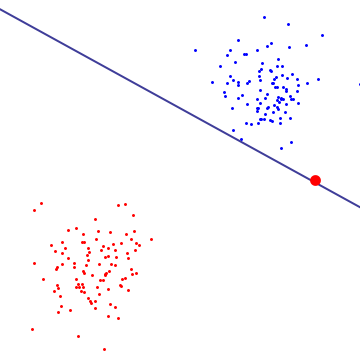
\includegraphics[width=0.50\textwidth]{figures/svm.png}
            \label{fig:svm_scenarios}
 \end{figure}
The second method, percentage classification, is an unsupervised mechanism and leads to segregation of data even if they are homogeneously distributed among the dataset. The percentage classification is interesting to be used in the scenarios similar to k-means, without the unpredictable of the original method.\\
This method is interesting when the standard deviations of the data are similar, so the result will be a reduced number of groups, even one group as result but might lead to many groups when the average distance of them is larger than a certain threshold. This method weave the solution of a specific problem to quantify the groups in a distribution, scenario 1, in the Figure 5.1. 
 
 \begin{figure}[h]
          \center
          \caption{Percentage Classification Scenarios}
            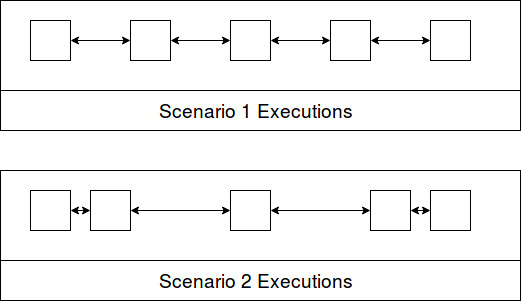
\includegraphics[width=0.90\textwidth]{figures/scenarios_percentage.jpg}
            \label{fig:scenarios_percentage}
    \end{figure}

Finally, the k-means algorithm is efficient but requires the number of groups to be used in the classification process, which cluster the data using a centroid. Still, k-means does not carry the exact same result at each run.
The k-means algorithm is specially interesting in scenarios such as: two or three main clusters. However, in scenarios where the data is homogeneously distributed and when there is just one cluster.
The scenarios described in Figure 5.2 are clear limitation of k-means algorithm. The first scenario is when the data is not suitable for this technique. In our experiments both were not found in the use cases, but could occur.\\
 
 \begin{figure}[h]
          \center
          \caption{K-means Scenarios }
            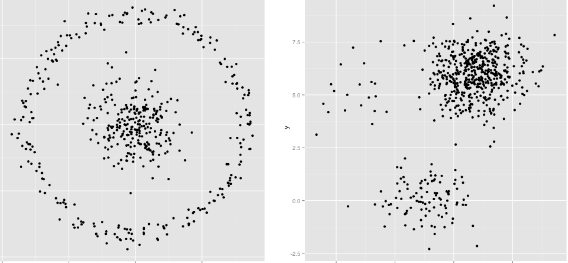
\includegraphics[width=0.90\textwidth]{figures/scenarios_k.png}
            \label{fig:scenarios_k}
    \end{figure}

The methods described on this work summarize a series of methods to measure differences among groups of execution. The data mining methods, i.e. SVM, k-means and percentage classification. On the other hand, the statistical method used in the solution can provide a relative comparison of the performance among the groups to specific indicate the metrics as a cause for issues.\\
The statistical tools can also be used to detect regressions, as the collaboration \cite{google_releases} showed, using confidence Interval to find regressions among Chromium releases. 
As final remarks in the comparison is whether the groups are well defined and where the anomalies are just not a new pattern in the data as listed in \cite{Chandola2009ADS15418801541882}. In this matter, each grouping technique, such as the percentage grouping, have its own borders definition.
\section{Results discussion}
The results were able to indicate specific metrics that might be used to improve a software performance. The solution can be used in two ways: as a detection tool or as analysis tool. In other words, in some cases the solution is able specifically to demonstrate where should be done the corrections in other cases the solution will give a guideline to a specific metric of the issue, i.e. a metric guidance that can be used by the developer to find the source code.\\
The example of OpenCV, it was possible to reduce the number of commits using the result in a specific function. However, it was necessary to consider the code of the application to do a complete analysis.\\
In other cases, the longer runs were related to specific metrics, e.g. cache misses, and the groups comparison was able to identify this information. The versions could then be compared considering this information, so the regressions test can be properly done.
\section{Metrics collision}
During the experiments we found that an overhead was added in due to the use of several performance metrics in the tracing method. Therefore, instead of recording all the metrics at the same time, it is possible to used an experiment setup that can be used to infer the influence of different metrics in a application. This setup is similar to psychology tests. \\
This method is not presented in the paper, since we were able to trace the applications with all the metrics enabled. Using the cross validation setup, the results can be summarized in the tables below:
\begin{table}[h]
\centering
\caption{Table Metric Association}
\label{tab:table1}
\begin{tabular}{lll}
\hline
Metric A              & Metric B   &     Metric C        \\ \hline
enabled & - & enabled \\ \hline
- & enabled & enabled \\ \hline
enabled & enabled & - 
\end{tabular}
\end{table}
 
Considering that the results are the following Table \ref{tab:table2}, the cross where the impact of BC is 40 percent and the impact of AB is 10 percent, the deduced impact of C must be no less than 20 percent.
    
\begin{table}[h]
\centering
\caption{Table Group Impact}
\label{tab:table2}
\begin{tabular}{ll}
\hline
Groups             &    Impact   \\ \hline
AB & 10 percent impact \\ \hline
AC & 40 percent impact \\ \hline
BC & 30 percent impact
\end{tabular}
\end{table}

It is possible therefore to construct an association rule to simplify this process and avoid tracing overhead unnecessarily.
\section{Auto clustering discussion}
Considering the models shown above, we chose to develop a non-supervised method, a.k.a auto clustering. The possibility to use an automated approach is more interesting for us in comparison with a non-automated methods, mainly because we aim not to use the data to train the model. \\
Therefore, we implemented a version of comparative k-means using the SSE (sum of square errors) variability information, plus a heuristic evaluation. This technique can be used for an arbitrary dimension of since the amount of difference, SSE (sum of squared error), can be calculated on those cases.  Some limitations apply on this approach and it is possible to use Gaussian Mixture Model to overcome them, as elaborated in \cite{gaussian}.\\
Since the SSE drops considerably between one group and two groups, we need always to consider more than two groups, otherwise the chosen gap will be two groups.
From the perspective of the Elbow method, also called silhouette method, which in fact is just of of the criteria that can be used to find the best k, as the calinski criterion as described in \cite{calinski}. This approach, Calinski-Harabasz,  is used in \cite{cluster} to specifically determine the number of clusters.\\
The used approach can also be compared with the x-means clustering technique, where the best results are kept to be compared.A more complete approach could be done using the gap statistical calculation, which uses calculation of within cluster dispersion, as described in \cite{gap_statistical}.
The next step would be to use an agglomerative clustering technique, which is an bottom up technique where each observation.

\section{Performance Counters}
The first highlight in the research are the performance counters used are limited to the counters in Perf. The more addition, the more overhead is added, so the use cross-validation scheme. 
Depending on the quantity of different metric counters, the process of grouping will increase its complexity, even hundreds of metrics as expressed in \cite{cluster}. \\
Besides, considering hundreds of metrics, a pair-wise analysis done in the groups comparison could be a restriction, consequently another a control chart could be used.
    
\section{Data structure evaluation}
We used two dynamic structures in the solution, a calling context tree with metrics, i.e. ECCT but also a dynamic call tree with metrics, i.e. EDT instead of a ECCT. 
The main difference resides in the summarized purpose of the ECCT, which is used in previous literature. Although the EDT has much longer size comparatively, the use of EDT is to avoid the addition of a pre-processing phase in the comparison of the internal nodes, that is, when comparing small portions of a software application, where an entire tree is unnecessary, the use of a EDT can be more suitable.\\
Those two dynamic structures, as any other tree, can be analyzed comparatively in two specific ways: the topological organization of the structure and the weights of the nodes. \\
The first approach can be used to compare differences among software, specifically targeting the profiling approaches. This strategy can be used in terms of tracing mining in kernel space if a pattern approach is used to automatically delimit the entries and exits of the nodes.\\
The second approach is the used in this research and consists of comparison of weights of nodes of similar trees. In this approach, the weights are the hardware and software performance metrics, e.g. page-faults and cache-misses.
\section{Usage}
This tool has various situations where the standard profiling is not suitable and the tracing requires analysis, for example with large data traces.
An unequivocal example of real utilization of this tool are regressions tests, as shown in the use cases of OpenCV and cache-misses. Though the proposed solution can be used to detect regressions, it is suitable as a diagnosis tool, since it can indicate root cause.\\
The solution presented in this research could be integrated to PARCS or even in a similar framework, while the performance metrics are compared in each version and see the patterns, since the mining technique have a complementary approach that compares the weights of the nodes, instead of the topological structure. \\
Although not explored, it is possible to use this work for developing enhanced trees, ECCTs or EDTs, in the kernel side of the system and applying the same comparison techniques explored here, it is possible to mine data from it.
\section{Visualization Tools}
The Red Grey Green Differential, RGG, suggested in the work can reduce the ambiguity of the similar executions, which would have the same color although they had different performances comparatively. \\
This different implementation, in comparison to the standard Differential Flame Graph, will reduce the analysis time by avoiding the verification of the equal time use cases. In terms of groups of event or profiling data in general.\\
We conclude this research through an evaluative summary of the contribution by considering several aspects of the proposed solution. First, we present a summary of the work, then, the objectives attainment, this is followed by the limitations of our solution and recommend future improvements.

             % Troisième thème (Doctorat) ou effacez ce fichier si vous êtes à la Maîtrise.
\Chapter{CONCLUSION}\label{sec:Conclusion}
We conclude this demonstration of the work by summarizing the contributions we have made. Then we present the limitations of our solution and recommend future improvements.

%%
%%  SYNTHESE DES TRAVAUX
%%
\section{Summary of the work}
The current tools are limited in terms of quantity of data to be analyzed and the so several data mining techniques can be applied to find associations and correlation among executions. This research aims to expand the current models by introducing an automated comparison mechanism. \\
The contribution through an automate mechanism using an heuristic evaluation to automate grouping techniques. The heuristic evaluation can be built upon several already used algorithms, such as k-means. Different strategies of comparison, such as the percentage comparison might highlight different behaviours of the system in a complementary way.\\
The proposed solution can compare the groups of executions with different performances and evaluate their inner structure using or not the source code as reference.


%%
%%  LIMITATIONS
%%
\section{Objective attainment}\label{sec:Limitations}
This work aimed to demonstrate the possibility to use automatic methods to reduce considerably the analysis time of performance comparison. The proposed solution, auto grouping mechanism presented in an article, enabled an automatic comparison of groups of executions and comparison of their behavior. Finally, the solution was able to be applied in several case studies demonstrating the effectiveness of the approach regarding to find performance issues with a group comparison strategy and that the challenge overall is surmountable.\\
%%
%%  AMELIORATIONS FUTURES
%%
\section{Contributions}
The scientific contributions for this work were summarized in the papers presented as and contains few contributions. \\
(1) We used an heuristic comparison to automate the current cluster and grouping mechanism without increasing excessively the complexity of those algorithms. Using this strategy, we were able to propose automatic way to compare several executions without necessarily selecting the number of groups that would be compared.\\
(2) Comparison of several clustering techniques, analyzing their pros and cons. This might be used in the future to improve their cons and improve those methods.\\ 
(3) We developed the RGG Differential flame graph, which can show differences on the executions in three colors reducing the ambiguity of the comparison of the original DFG. This is an new view that allows comparison of two groups of executions. \\
(4) In co-authorship we applied Confidence Interval using medians, instead of means, to compare several releases of Chromium software. This technique overpassed the current CI implementations.

\section{Limitations of the solution}
The auto grouping technique has two main limitations: the causation and the optimal number of groups.
First, is that association with the group analysis does not necessarily imply in causation, since correlation does not mean causation. A more deep evaluation would be necessary to study the causality and its association with the performance counters in terms of real percentage of representation and causation.\\
Second limitation in the auto-grouping, as well as group analysis in general, is the optimal number of groups which not necessarily can facilitate the human analysis of the system. A few times the number of groups is particularly large and although the number is optimal, it does not necessarily is the best number in terms of performance analysis.

\section{Future Work}
In the future it is possible to develop a fully automatic analysis framework, that include trace correlation, comparison and statistical analysis. 
This work showed the possibility to use fuzzy data, i.e. more than two groups of comparison automatically, however a deep analysis in each metric could be done to verify and measure specifically the impact of each performance variation in the runs in real workloads. 
An promising area is to use a neural network or other technique to correlate the user space tracing with kernel space tracing could give interesting aspects of performance evaluation. Technique that does not require labeled data can be used also.
From the implementation part, the solution was implemented focusing in userspace tracing library and can only capture the stack for ELF binaries. Therefore, it should be extended to address other needs such as JIT compilation.


         % Conclusion.
%\backmatter
\renewcommand\bibname{RÉFÉRENCES}
\bibliography{Document}
\bibliographystyle{polymtl}  % Format de la bibliographie.
\bibliographystyle{IEEEtranSN-francais}  % Format de la bibliographie.
% %
% \ifthenelse{\equal{\AnnexesPresentes}{O}}{
% \appendix%
% \newcommand{\Annexe}[1]{\annexe{#1}\setcounter{figure}{0}\setcounter{table}{0}\setcounter{footnote}{0}}%
% %%
%%  Annexes.
%%
%%  Note: Ne pas modifier la ligne ci-dessous.
\addcontentsline{toc}{compteur}{ANNEXES}
%%
%%
%%  Toutes les annexes doivent être inclues dans ce document
%%  les unes à la suite des autres.
\Annexe{DÉMO}
Texte de l'annexe A\@. Remarquez que la phrase précédente se termine
par une lettre majuscule suivie d'un point. On indique explicitement
cette situation à \LaTeX{} afin que ce dernier ajuste correctement
l'espacement entre le point final de la phrase et le début de la
phrase suivante.


\begin{landscape}
\Annexe{ENCORE UNE ANNEXE}
Texte de l'annexe B\@ en mode «landscape».
\end{landscape}

\Annexe{UNE DERNIÈRE ANNEXE}
Texte de l'annexe C\@.
}{}
\end{document}
